%-----------------------------------------------%
% abnTeX2: Modelo de Trabalho Academico em conformidade com 
% ABNT NBR 14724:2011: Informacao e documentacao - Trabalhos academicos -
% Apresentacao
%
% Adaptado por Rodrigo Nascimento (2022-08-12) modelo baseado no 
% https://github.com/emersonmello/modelos-latex/tree/master/monografia
% criado pelo professor Emerson Mello (IFSC)
%-----------------------------------------------%

\documentclass[
	% -- opções da classe memoir --
	12pt,				% tamanho da fonte0
	openright,			% capítulos começam em pág ímpar (insere página vazia caso preciso)
	oneside,			% twoside para impressão em verso e anverso. Oposto a oneside
	a4paper,			% tamanho do papel. 
	% -- opções da classe abntex2 --
	%chapter=TITLE,		% títulos de capítulos convertidos em letras maiúsculas
	%section=TITLE,		% títulos de seções convertidos em letras maiúsculas
	%subsection=TITLE,	% títulos de subseções convertidos em letras maiúsculas
	%subsubsection=TITLE,% títulos de subsubseções convertidos em letras maiúsculas
	% -- opções do pacote babel --
	english,			% idioma adicional para hifenização
%	french,				% idioma adicional para hifenização
%	spanish,			% idioma adicional para hifenização
	brazil				% o último idioma é o principal do documento
]{abntex2}

%-----------------------------------------------%
% Informações de dados para CAPA e FOLHA DE ROSTO
%-----------------------------------------------%
\instituicao{Universidade do Estado de Santa Catarina -- UDESC}
\titulo{Estágio Curricular Supervisionado -- IV}
\autor{Rodrigo Nascimento}
\local{Joinville - SC}
\data{\mydate}
\tipotrabalho{Plano de Aula}
\orientador{Prof(a). Dr(a). Ana P. Grimes de Souza}
\coorientador{Prof. Me. Mário Heleno Calegari}
%-----------------------------------------------%
% Para alterar o parâmetros dos comandos orientador
% e coorientador.
%-----------------------------------------------%
% \renewcommand{\orientadorname}{Orientadora:}
\renewcommand{\coorientadorname}{Supervisor:}
%-----------------------------------------------%

\newcommand{\centro}{Centro de Ciências Tecnológicas -- CCT }
\newcommand{\departamento}{Departamento de Física -- DFIS}
\newcommand{\curso}{Licenciatura em Física }
\newcommand{\disciplina}{Estágio Curricular Supervisionado IV-- ESC4003}
\newcommand{\firstkey}{Estágio Supervisionado}
\newcommand{\secondkey}{Ensino de Física}
\newcommand{\thirdkey}{Ensino Médio}


%-----------------------------------------------%

%	Todas as indicações de pacotes e configurações estão no arquivo de estilo
%  chamado estilo-monografia-udesc.sty.
\usepackage{texmodel-udesc-b}

%-----------------------------------------------%
% Estilo de cabeçalho que só contém o número da 
% página e uma linha
%-----------------------------------------------%
\makepagestyle{cabecalholimpo}
\makeevenhead{cabecalholimpo}{\thepage}{}{} % páginas pares
\makeoddhead{cabecalholimpo}{}{}{\thepage} % páginas ímpares
%\makeheadrule{cabecalholimpo}{\textwidth}{\normalrulethickness} % linha
%-----------------------------------------------%

%-----------------------------------------------%
% Início do documento
%-----------------------------------------------%
\begin{document}

% Seleciona o idioma do documento (conforme pacotes do babel)
\selectlanguage{brazil}
% Retira espaço extra obsoleto entre as frases.
\frenchspacing
%-----------------------------------------------%
% ELEMENTOS PRÉ-TEXTUAIS
%-----------------------------------------------%
\pretextual
\imprimircapa
%-----------------------------------------------%
% No arquivo abaixo tem detalhes sobre folha de
% aprovação, ficha catalográfica, agradecimentos,
% resumo, abstract, etc.
% 
% Se não for a versão final do PDF, talvez fosse
% interessante comentar a linha abaixo.
%-----------------------------------------------%
% Folha de rosto - (o * indica que haverá a ficha bibliográfica)

%-----------------------------------------------%
% ARQUIVOS PRETEXTUAIS
% ----------------------------------------------%
\imprimirfolhaderosto*

%\includepdf{aprovacao.pdf}
%-----------------------------------------------%
% Inserir a ficha bibliografica %
%-----------------------------------------------%
% Isto é um exemplo de Ficha Catalográfica, ou ``Dados internacionais de
% catalogação-na-publicação''. Você pode utilizar este modelo como referência. 
% Porém, provavelmente a biblioteca da sua universidade lhe fornecerá um PDF
% com a ficha catalográfica definitiva após a defesa do trabalho. Quando estiver
% com o documento, salve-o como PDF no diretório do seu projeto e substitua todo
% o conteúdo de implementação deste arquivo pelo comando abaixo:
%
% \begin{fichacatalografica}
%     %\includepdf{fig_ficha_catalografica.pdf}    
% \end{fichacatalografica}

% ------------------------------
%EXEMPLO DE FICHA CATALOGRÁFICA
% ------------------------------
% \begin{fichacatalografica}
% 	\sffamily
% 	\vspace*{\fill}					% Posição vertical
% 	\begin{center}					% Minipage Centralizado
%         \fbox{
%             \begin{minipage}[c][8cm]{13.5cm}		% Largura
%                 \small
%                 \imprimirautor
%                 %Sobrenome, Nome do autor
                
%                 \hspace{0.5cm} \imprimirtitulo  / \imprimirautor. --
%                 \imprimirlocal, \imprimirdata-
                
%                 \hspace{0.5cm} \pageref{LastPage} p. : il. (algumas color.) ; 30 cm.\\
                
%                 \hspace{0.5cm} \imprimirorientadorRotulo~\imprimirorientador\\
                
%                 \hspace{0.5cm}
%                 \parbox[t]{\textwidth}{\imprimirtipotrabalho~--~\imprimirinstituicao,
%                 \imprimirdata.}\\
                
%                 \hspace{0.5cm}
%                     1. \firstkey.
%                     2. \secondkey.
%                     2. \thirdkey.
%                     I. Orientador.
%                     II. Universidade do Estado de Santa Catarina.
%                     III. \centro.
%                     IV. Título.
%             \end{minipage}
%         }
% 	\end{center}
% \end{fichacatalografica}
%-----------------------------------------------%

%-----------------------------------------------%
% Inserir folha de aprovação
%-----------------------------------------------%

% Isto é um exemplo de Folha de aprovação, elemento obrigatório da NBR
% 14724/2011 (seção 4.2.1.3). Você pode utilizar este modelo até a aprovação
% do trabalho. Após isso, substitua todo o conteúdo deste arquivo por uma
% imagem da página assinada pela banca com o comando abaixo:
%
% \includepdf{folhadeaprovacao_final.pdf}
 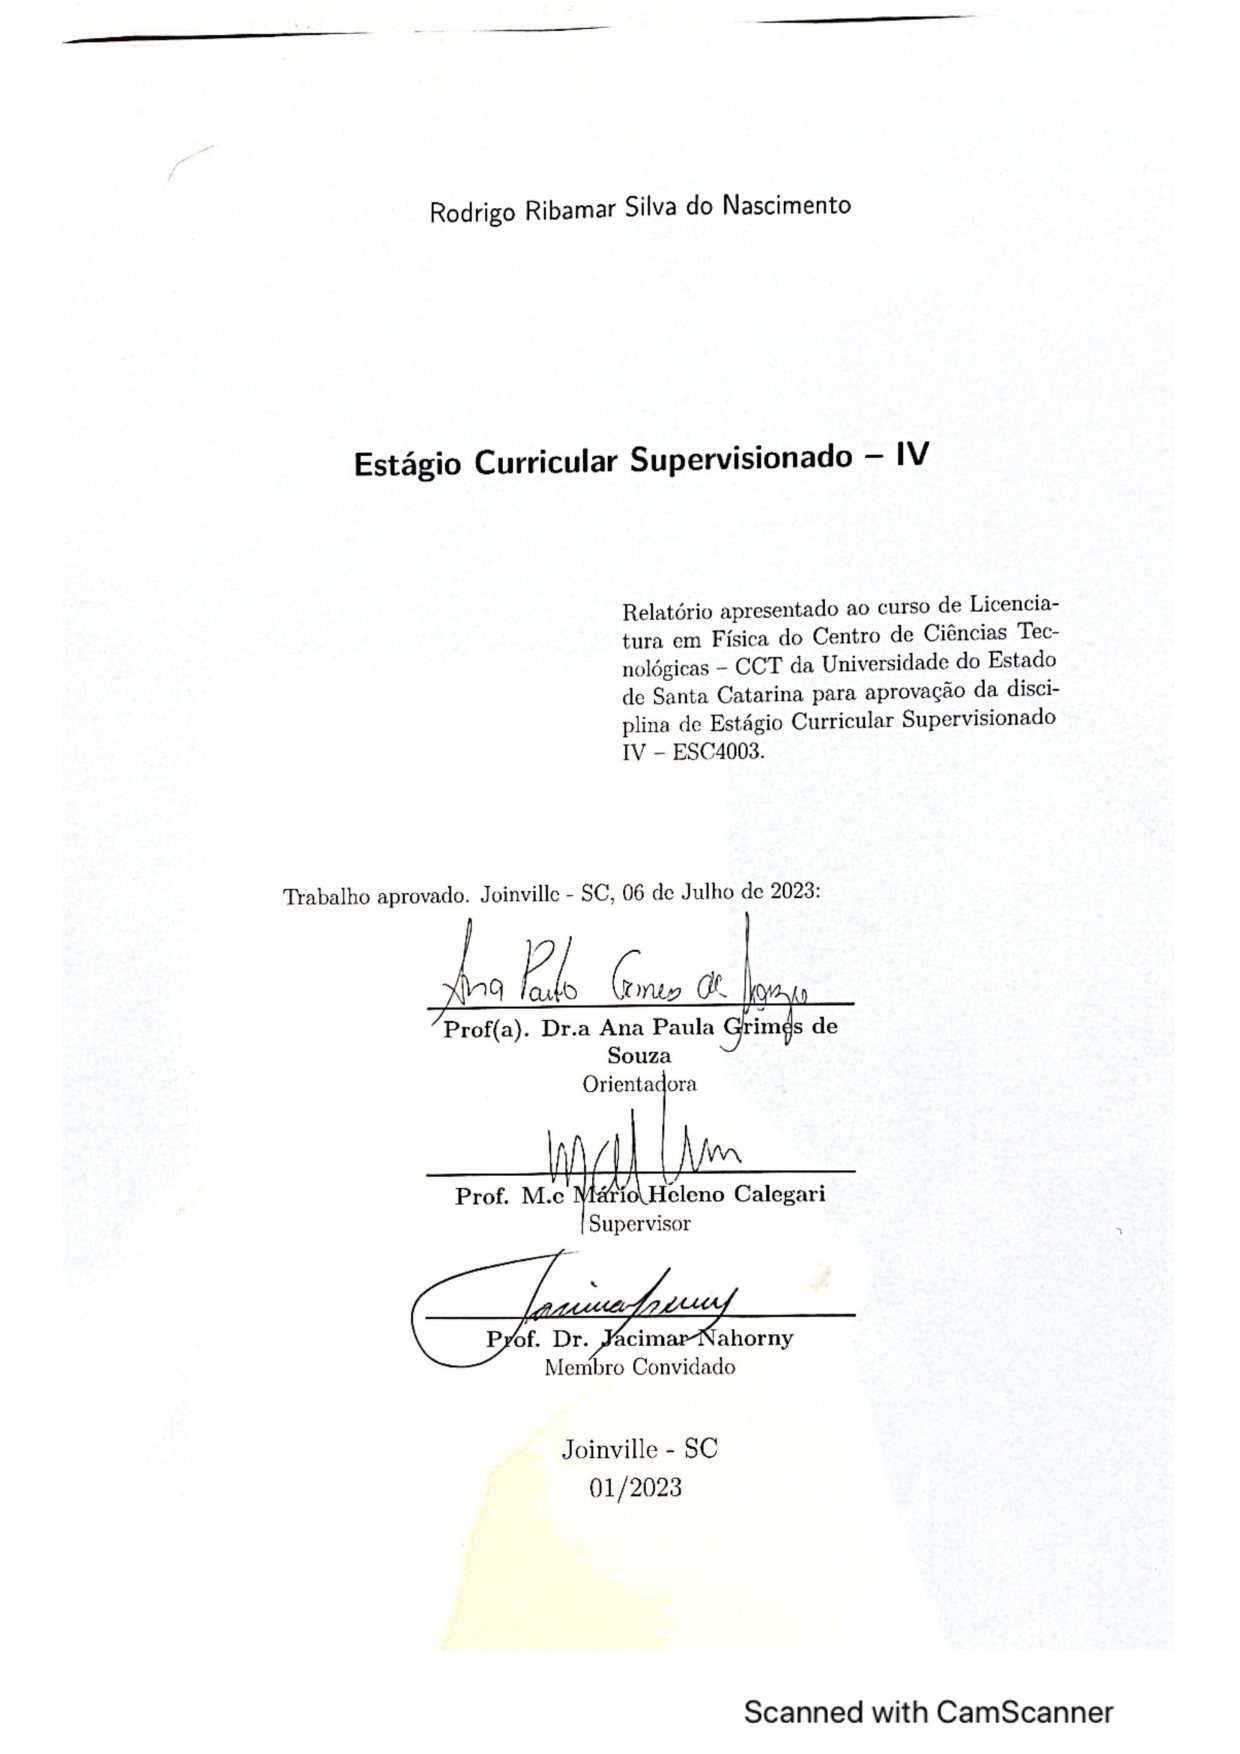
\includepdf[pages=-]{03-elementos/03.1_pre-textual/documentos_merged.pdf}
%
% \begin{folhadeaprovacao}
%     \textoaprovacao{Este trabalho foi julgado adequado para obtenção do título de Engenheiro de Telecomunicações, pelo Instituto Federal de Educação, Ciência e Tecnologia de Santa Catarina, e aprovado na sua forma final pela comissão avaliadora abaixo indicada.}
%     \begin{center}
%         {\ABNTEXchapterfont\large\MakeUppercase{\imprimirautor}}

%         \vspace*{\fill}\vspace*{\fill}
%         \begin{center}
%             \ABNTEXchapterfont\bfseries\Large\MakeUppercase{\imprimirtitulo}
%         \end{center}
%         \vspace*{\fill}
    
%         \imprimirtextoaprovacao
     
%         \vspace*{1cm}
    
% 	    \imprimirlocal, 6 de maio de 2021:

%     \vspace*{\fill}
%    \end{center}
        


%    \assinatura{\textbf{\imprimirorientador} \\ Orientador\\Instituto Federal de Santa Catarina} 
%    \assinatura{\textbf{Professor Fulano, Dr.} \\ Instituto X }
%    \assinatura{\textbf{Professora Fulana, Dra. } \\ Instituto Y}
%    \assinatura{\textbf{Professor Beltrano, Dr.} \\ Instituto Z}
%    \assinatura{\textbf{Professor} \\ Convidado 4}
      
%     \vspace*{1cm}  
  
% \end{folhadeaprovacao}
%-----------------------------------------------%
%-----------------------------------------------%
% Dedicatória
%-----------------------------------------------%
%
\begin{dedicatoria}
    \vspace*{\fill}    
    \begin{flushright}
        \noindent
        \textit{ Dedico este trabalho à minha namorada\\Laura Cordoba Zandonadi, cujo a\\barriga, habita um dinossauro.}\vspace*{2cm}
    \end{flushright}
\end{dedicatoria}
% ---
% Agradecimentos
%-----------------------------------------------%
%\begin{agradecimentos}
    Os agradecimentos principais são direcionados à Gerald Weber, Miguel Frasson,
    Leslie H. Watter, Bruno Parente Lima, Flávio de Vasconcellos Corrêa, Otavio Real
    Salvador, Renato Machnievscz\footnote{Os nomes dos integrantes do primeiro
    projeto abn\TeX\ foram extraídos de
    \url{http://codigolivre.org.br/projects/abntex/}} e todos aqueles que
    contribuíram para que a produção de trabalhos acadêmicos conforme
    as normas ABNT com \LaTeX\ fosse possível.
    
    Agradecimentos especiais são direcionados ao Centro de Pesquisa em Arquitetura
    da Informação\footnote{\url{http://www.cpai.unb.br/}} da Universidade de
    Brasília (CPAI), ao grupo de usuários
    \emph{latex-br}\footnote{\url{http://groups.google.com/group/latex-br}} e aos
    novos voluntários do grupo
    \emph{\abnTeX}\footnote{\url{http://groups.google.com/group/abntex2} e
    \url{http://www.abntex.net.br/}}~que contribuíram e que ainda
    contribuirão para a evolução do \abnTeX.    
\end{agradecimentos}
% ---
% Epígrafe
%-----------------------------------------------%
%\begin{epigrafe}
    \vspace*{\fill}
	\begin{flushright}
		\textit{Sempre que te perguntarem se podes fazer um trabalho,\\
		respondas que sim e te ponhas em seguida a aprender como se faz.\\
		T. Roosevelt}
	\end{flushright}
\end{epigrafe}
% ---


%-----------------------------------------------%
% RESUMO
%-----------------------------------------------%
\setlength{\absparsep}{18pt} % ajusta o espaçamento dos parágrafos do resumo
\begin{resumo}
    Relatório de estágio desenvolvido na Escola de Educação Básica Giovani Pasqualini Faraco no decorrer do segundo semestre do ano letivo de 2022. Dentre as atividades realizadas e aqui descritas, tem-se: a análise dos documentos oficiais da instituição; observação e análise de aulas da disciplina de Física ministradas pelo professor supervisor além de um plano de docência de oito aulas programadas, sob orientação e supervisionamento técnico. A cada etapa buscou-se o embasamento na literatura envolvida sempre em consonância com os documentos norteadores da educação básica do país.

\textbf{Palavras-chave}: \firstkey ; \secondkey ; \thirdkey.
\end{resumo}
%-----------------------------------------------%
% ABSTRACT
%-----------------------------------------------%
%\begin{resumo}[Abstract]
    \begin{otherlanguage*}{english}
      This is the english abstract.
   
      \vspace{\onelineskip}
    
      \noindent 
      \textbf{Keywords}: Latex. Abntex. Text editoration.
    \end{otherlanguage*}
\end{resumo}
%-----------------------------------------------%
% ------------------------
% ------------------------
% inserir SUMARIO E LISTAS
% -----------------------------------------------%
% inserir lista de ilustrações, tabelas, listagem 
% de códigos, abreviaturas, símbolos
% -----------------------------------------------%
% \pdfbookmark[0]{\listfigurename}{lof}
% \listoffigures*
% \cleardoublepage
% -----------------------------------------------%
% inserir lista de TABELAS
% -----------------------------------------------%
\pdfbookmark[0]{\listtablename}{lot}
\listoftables*
\cleardoublepage

% -----------------------------------------------%
% inserir lista de QUADROS
% -----------------------------------------------%
\pdfbookmark[0]{\listofquadrosname}{loq}
\listofquadros*
\cleardoublepage

% -----------------------------------------------%
% inserir lista de CÓDIGOS
% -----------------------------------------------%
% \pdfbookmark[0]{\lstlistlistingname}{lol}
% \begin{KeepFromToc}
% \lstlistoflistings
% \end{KeepFromToc}
% \cleardoublepage
% -----------------------------------------------%

% -----------------------------------------------%
% inserir lista de abreviaturas e siglas
% -----------------------------------------------%
\pdfbookmark[0]{Lista de abreviaturas e siglas}{loa}
%%%%%%%%%%%%%% Como usar o pacote acronym
% \ac{acronimo} -- Na primeira vez que for citado o acronimo, o nome completo irá aparecer
%                  seguido do acronimo entre parênteses. Na proxima vez somente o acronimo
%                  irá aparecer. Se usou a opção footnote no pacote, entao o nome por extenso
%                  irá aparecer aparecer no rodapé
%
% \acf{acronimo} -- Para aparecer com nome completo + acronimo
% \acs{acronimo} -- Para aparecer somente o acronimo
% \acl{acronimo} -- Nome por extenso somente, sem o acronimo
% \acp{acronimo} -- igual o \ac mas deixando no plural com S (ingles)
% \acfp{acronimo}--
% \acsp{acronimo}--
% \aclp{acronimo}--


\chapter*{Lista de abreviaturas e siglas}%
% \addcontentsline{toc}{chapter}{Lista de abreviaturas e siglas}
\markboth{Lista de abreviaturas e siglas}{}

% Para diminuir o espaçamento entre linhas no ambiente de listas acronym
% \let\oldbaselinestretch=\baselinestretch%
% \renewcommand{\baselinestretch}{.2}%
% \large\normalsize%



\begin{acronym}
	\let\oldbaselinestretch=\baselinestretch%
	\renewcommand{\baselinestretch}{.2}%
	\large\normalsize%
	\acro{BNCC}{Base Nacional Comum Curricular}
	\acro{LDB}{Lei de Diretrizes de Bases da Educação Nacional}
	\acro{NEM}{Novo Ensino Médio}
	\acro{PCSC}{Proposta Curricular de Santa Catarina}
	\acro{PNE}{Plano Nacional de Educação}
	\acro{CNE}{Conselho Nacional de Educação}
	\acro{EEB}{Escola de Educação Básica}
	\acro{GPF}{Giovani Pasqualini faraco}
	\acro{EF}{Ensino Fundamental}
	\acro{PPP}{Projeto Político Pedagógico}
	\acro{ATP}{Assistente Técnico Pedagógico}
	\acro{DVD}{\textit{Digital Versatile Disc}}
	\acro{EI}{Ensino por Investigação}
	\acro{NI/D}{Não-Interativo/Dialógico}
	\acro{I/D}{Interativo-Dialógico}
	\acro{HC}{História da Ciência}
	\acro{TIC}{Tecnologia da Informação e Comunicação}
	\acro{ENEM}{Exame Nacional do Ensino Médio}
	\acro{I/DA}{Interativo/Dialógico de Autoridade}
        \acro{BBTD}{Biblioteca Brasileira de Teses e Dissertações}
        \acro{MEC}{Ministério da Educação}
        \acro{MNPEF}{Mestrado Nacional Profissional em Ensino de Física}
        \acro{ICEX}{Instituto de Ciências Exatas}
        \acro{UFF}{Universidade Federal Fluminense}
        \acro{HFC}{História e Filosofia da Ciência}
\end{acronym}

\cleardoublepage
% -----------------------------------------------%

% -----------------------------------------------%
% inserir lista de símbolos
% -----------------------------------------------%
\begin{simbolos}  
  \item[$\Delta$] Variações de Grandezas Físicas
  \item[$X_i$] Medida Inicial da Grandeza $X$
  \item[$L$] Grandeza Física Associada ao Comprimento
  \item[$\alpha$] Coeficiente de Dilatação Linear
  \item[$T$] Grandeza Física Associada a Temperatura
  \item[$A$] Grandeza Física Associada a Área Superficial
  \item[$\beta$] Coeficiente de Dilatação Superficial
  \item[$V$] Grandeza Física Associada ao Volume
  \item[$\gamma$] Coeficiente de Dilatação Volumétrica 
  \item[$X_f$] Medida final da Grandeza $X$
\end{simbolos}
% -----------------------------------------------%

% -----------------------------------------------%
% inserir o SUMÁRIO
% -----------------------------------------------%
\pdfbookmark[0]{\contentsname}{toc}
\tableofcontents*
\cleardoublepage
% -----------------------------------------------%
% ------------------------

%-----------------------------------------------%
% ELEMENTOS TEXTUAIS
%-----------------------------------------------%
\textual
% Se quiser que apareça o título dos capítulos
% no cabeçalho, então comente a linha abaixo
%\pagestyle{cabecalholimpo}
%-----------------------------------------------%
% Inclusão dos capítulos que estão em outros arquivos .tex
%-----------------------------------------------%
%============| INÍCIO |=======================================>
\chapter{Introdução}
\thispagestyle{empty}
\label{cap:Introducao}

\lettrine{D}{esde} o seu surgimento no século XI o termo estágio \emph{(do lat.: stagium)} tem sido associado à aprendizagem posta em prática num local adequado e sob supervisão \cite{COLOMBO:2014}. Durante a trajetória acadêmica, os saberes adquiridos ao longo dos anos de formação são postos em prática buscando estabelecer vínculos entre o saber e o saber fazer, acompanhado por um profissional da área que orientará e corrigirá as ações desenvolvidas pelo estagiário e assim, evitar falhas no exercício de suas atribuições no momento em que estiver apto a desenvolvê-las.

Neste sentido os estágios representam para o estagiário uma oportunidade de colocar em prática os conhecimentos construídos pelo futuro profissional ao longo de todo o processo formativo. Esta prática é tanto mais proveitosa quando proporcionada à situações concretas e próximas da realidade profissional. Embora nestes termos não esteja explicitado, vale ressaltar que a prática do estágio jamais deve ser confundida com aplicação de mão de obra barata. A Lei de n$^\circ$ 11.788, de 25 de setembro de 2008 determina que o estágio seja vinculado puramente ao processo educativo. O conhecimento da norma e a gestão correta do estágio pelas instituições devem ser suficientes para evitar que esta prática se difunda na forma de precarização das relações do trabalho.

\section{Documentos Norteadores da Educação Nacional}
Com a homologação da 3ª versão da \ac{BNCC} em dezembro de 2017, passa então a valer em todo o território nacional, em caráter compulsório e de forma prevista pela \ac{LDB} assim como no \ac{PNE}, as políticas educacionais voltadas a orientar a elaboração: dos currículos locais, da formação inicial e continuada dos professores, do material didático, da avaliação e do apoio pedagógico aos alunos \cite{BRASIL:2017}, a fim de assegurar e promover os direitos de aprendizagem essenciais aos educandos com vistas à formação humana integral e à construção de uma sociedade justa, democrática e inclusiva.

O texto tem como foco o desenvolvimento de \emph{competências} por meio das quais o educando, ao longo de todo o processo formativo, deva ser capaz de:

\begin{citacao}
    ``\ldots aprender a aprender, saber lidar com a informação cada vez mais disponível, atuar com discernimento e responsabilidade nos contextos das culturas digitais, aplicar conhecimentos para resolver problemas, ter autonomia para tomar decisões, ser proativo para identificar os dados de uma situação e buscar soluções, conviver e aprender com as diferenças e as diversidades.'' 
    \Ibidem[p. ~14]{BRASIL:2017}   
\end{citacao}
Excepcionalmente no ano de escrita deste relatório, as escolas de Santa Catarina iniciaram o processo de implementação da \ac{BNCC} no então denominado \ac{NEM}. Vem então direcionando esforços para adequar a medida primeiramente a todas as turmas de primeiro ano e tendo por pretensão concluir o processo até o ano de 2024, ano em que deve-se incluir as turmas de terceiro ano.

Não obstante, Santa Catarina também possui a sua proposta para a educação básica. O Estado é, aliás, pioneiro na definição de diretrizes curriculares e, desde 1988, vem elaborando e (re)elaborando a sua proposta em participação conjunta com diversos profissionais dos segmentos educativos. A \ac{PCSC} em sua versão mais recente, cita três elementos norteadores que orientaram a consolidação do modelo atual, como sendo a:

\begin{citacao}
    ``1) perspectiva de formação integral, referenciada numa concepção multidimensional de sujeito; 2) concepção de percurso formativo visando superar o etapismo escolar e a razão fragmentária que ainda predomina na organização curricular e 3) atenção à concepção de diversidade no reconhecimento das diferentes configurações identitárias e de novas modalidaes de educação \cite[p.~20]{PCSC:2014}''
\end{citacao}
Em atenção a estes elementos, a proposta ainda orienta a formação dos currículos e do \ac{PPP} no sentido de promover a:

\begin{citacao}
    ``Superação do etapismo no percurso formativo; promoção do diálogo entre as diferentes áreas do conhecimento, sem deixar de considerar as especificidades das áreas e dos componentes curriculares; escolhas teórico-metodológicas, de conhecimentos e de experiências significativas para compor o percurso formativo e que mobilizem os sujeitos para a aprendizagem; reconhecimento da diversidade de identidades e de saberes como condição político-pedagógica para o desenvolvimento da Educação Básica; ampliação de espaços de autonomia intelectual e política dos sujeitos envolvidos nos percursos formativos; exploração das interfaces entre os saberes, dos \emph{entre-lugares (sic)}, das redes, das coletividades como \emph{lócus} geradores de conhecimento; democratização da gestão dos processos educativos pela valorização e fortalecimento do trabalho coletivo \opcit[p.~27]{PCSC:2014}''
\end{citacao}

Assim, estabelece uma concepção de currículo \emph{``\ldots mutável, ou seja, ações pedagógicas que propiciem ao sujeito ser ativo em situações de pesquisa, referente ao objeto de estudo''}, destacam \cite[p.~409]{COMIOTTO:2021}. Como podemos observar, ambas as propostas atuam de forma complementares sendo ainda concordantes em muitos aspectos. Tanto a \ac{BNCC} quanto a \ac{PCSC} formam as bases legais e norteadoras da educação catarinense e o seu conhecimento é de fundamental importância para o exercício do profissional de educação que irá atuar no Estado.

Face a isso, os cursos de licenciaturas do país têm buscado promover, nos currículos de graduação, o conjunto de ações adequadas a atender às exigências dos documentos norteadores. Neste processo, encontram-se as disciplinas de Estágio Curricular Supervisionado I/II/III e IV, responsáveis por oportunizar uma primeira aproximação do acadêmico com a carreira docente em ambiente escolar supervisionado, sendo um componente curricular obrigatório e indispensável nos cursos de licenciatura, de acordo com a resolução \cite{BRASIL:2002a} homologada pelo \ac{CNE} na forma do parecer de nº  CNE/CP nº 1, de 18 de Fevereiro de 2002.

\section{Referenciais Teórico-Metodológico}

Longe de reduzir a ação dos docentes a meros agentes tecnicistas, limitados a cumprir passivamente o que lhes ditam verticalmente, vê-se nos textos das Bases, uma proximidade com as concepções da filosofia \emph{deweyana}\footnote{John Dewey (1859-1952), filósofo americano que influenciou educadores de várias partes do mundo e que no Brasil inspirou o \emph{Movimento da Escola Nova}, liderado por Anísio Teixeira.}, e neste sentido, considera-se o movimento da \emph{Prática Reflexiva} proposta por \cite{ZEICHNER:1993} como elemento catalisador do pensar e repensar frequentemente a prática pedagógica. Para o autor:

\begin{citacao}
``O conceito de professor como prático reflexivo reconhece a riqueza da experiência que reside na prática dos bons professores. Na perspectiva de cada professor, significa que o processo de compreensão e melhoria do seu ensino deve começar pela reflexão sobre a sua própria experiência e que o tipo de saber inteiramente tirado da experiência dos outros (mesmo de outros professores) é, no melhor dos casos, pobre e, no pior, ilusão.'' \opcit[p. ~17]{ZEICHNER:1993}
\end{citacao}
Não se trata aqui de tornar o estagiário durante o exercício do estágio, um crítico contumaz à pratica docente observada em sala de aula, mas sim de fazê-lo

\begin{citacao}
``[...]detectar e superar uma visão simplista dos problemas de ensino e aprendizagem, proporcionando dados significativos do cotidiano escolar que possibilitem uma \textbf{reflexão crítica} do trabalho a ser desenvolvido como professor e dos processos de ensino e aprendizagem em relação ao seu conteúdo específico.'' \cite[p. 11, \textbf{grifos meus}]{CARVALHO:2012} 
\end{citacao}
Assim sendo, as problematizações trazidas à tona neste trabalho, só tem sentido se vistas no âmbito de elucidar a complexa relação existente entre o ato de ensinar e a aprendizagem significativa desejada, à luz destes referenciais.

\section{Contexto}
Este estágio foi desenvolvido ao longo do segundo semestre do ano de 2022, na \ac{EEB} \ac{GPF}, para a disciplina de \disciplina \; do curso de Licenciatura em Física, em que o estagiário é convidado a desenvolver atividades relacionadas à caracterização do ambiente escolar, acompanhamentos de aulas, além de proposição e execução de atividades imersivas.
 
O restante desse trabalho está organizado da seguinte maneira: no \autoref{cap: aprConcedente} é apresentada a unidade concedente do estágio, suas características estruturais e organizacionais; o \autoref{cap: apoioDocencia} é destinado a apresentação dos programas de apoio à docência; no \autoref{cap: prgFisica} faremos a apresentação dos programas da disciplina de Física;... [continua] %no \autoref{cap: acmpDeAulas} apresentaremos o acompanhamento das aulas assistidas; as intervenções feitas em sala de aula encontram-se no \autoref{cap: docCompartilhada} e por fim, as considerações finais serão apresentados no  \autoref{cap: consideracoesFinais}.

%=============| FIM |=========================================>
\chapter{Apresentação da Concedente}
\thispagestyle{empty}
\label{cap: aprConcedente}

Um estudo elaborado por \cite{CARVALHO:2012} recomenda aos estagiários a tomarem conhecimento do ambiente escolar primeiramente por intermédio da observação. Buscando entre uma observação e outra compreender a realidade a que estará inserido no decorrer de sua atuação profissional, em tese isso deve contribuir para orientar a prática pedagógica do futuro professor e fornecer-lhes dados subsidiários, para uma formação sólida e humanizada.

\begin{citacao}
``O conhecimento de uma escola passa pelo conhecimento de sua parte física e humana.(...)mas principalmente com a sua sensibilidade (do estagiário). Ela é limpa? É um ambiente agradável fisicamente? Um membro da equipe diretora está sempre presente na escola?'' \Ibidem[p. ~5]{CARVALHOAMP:2012a}
\end{citacao}
Adotando esta recomendação, dar-se-á por iniciada nossas atividades.

\section{Caracterização da Unidade Escolar}
De muros altos e pintados de verde a Escola Giovani Pasqualini Faraco se mistura à paisagem urbana da região norte de Joinville e não passa despercebida, pois tudo em sua estrutura, ainda que de certa forma escondida pelos muros, revela o padrão estrutural das unidades escolares públicas da região. Em tinta branca e em caixa alta é lido o nome da escola numa parte do muro e, dessa forma, os muros não apenas lhe conferem \emph{proteção}, mas também referência.

O acompanhamento dos muros nos leva a entrada principal, consiste num portão largo, aberto ao início e final de cada turno, é por onde passam a maioria dos alunos, um segundo portão feito de grade e estreito é visto mais adiante, este da acesso à secretaria. De clima agradável, muito bem equipada e limpa a secretaria é a primeira instância administrativa de que a comunidade tem acesso direto à escola, há sempre alguém de prontidão e não demora muito a atendê-lo. Folhetos no balcão e cartazes colados nos murais, informam as datas e atividades que a escola desenvolve em conjunto com a comunidade. Um caminho estreito e florido, liga a secretaria ao hall onde ficam: as salas dos(as) Assistentes Técnicos(os) Pedagógicas(os), da Direção e a dos Professores.

A unidade funciona nos três turnos disponíveis, atende desde o 1º ao 9º ano do \ac{EF} e do 1º ao 3º ano do \ac{NEM}.

\subsection{Histórico}
Fundada em 15 de fevereiro de 1938, a Escola Desdobrada Dona Francisca Quilômetro Cinco, fica situada junto à Rua Dona Francisca, número 4957, Bairro Santo Antônio, Joinville/SC. Têm em seu nome o Patrono da instituição, \emph{Giovani Faraco}.

Nascido em 05 de abril de 1915, filho de Biase Faraco e Maria Limongi Faraco, conclui o Ensino Primário na Escola São José, ingressando em seguida no Ginásio onde permanece como aluno interno até o ano de 1929. Em 1930 entra pro Seminário Central de São Leopoldo, onde permanece até o ano de 1935. Ao passo de sua jornada, lecionou latim e português em diversos estabelecimentos particulares. Possui boa desenvoltura musical e compôs várias partituras para o instrumento órgão. Falece em 10 de novembro de 1960, vítima de hipertensão arterial, deixando sua esposa Tusnelda Gomes Faraco e cinco filhos.

O decreto de n$^\circ$ 10138/70 renomeia a unidade para Grupo Escolar Giovani Pasqualini Faraco e em 08 de junho de 1993, recebe aprovação do Conselho Estadual de Educação para implantar o Ensino Médio através do parecer de n$^\circ$ 117/93. Atualmente integra a rede Estadual de Ensino sob o nome Escola de Educação Básica Giovani Pasqualini Faraco.

\subsection{Infraestrutura}
Tem por área construída 3114,50$\m^2$ e outros 13929,25$\m^2$ de área disponível. Conta com uma infraestrutura de: 17 salas de aulas de 42$\m^2$ cada, cozinha, depósito para merenda escolar, depósito para produtos de limpeza, cantina, banheiros feminino e masculino, banheiros para professores, biblioteca, laboratório para as disciplinas de Física/Química e Biologia, laboratório de informática, sala ambiente para a disciplina de língua Portuguesa, arquivo inativo, sala para materiais de Educação Física, sala para materiais e equipamentos de: orientação escolar, direção, vídeo, artes e materiais para docentes.

A área descoberta é bem agradável e limpa, possui árvores ao seu redor criando um ambiente convidativo para o exercício da leitura, recreação ou até mesmo aulas diversificadas. Possui também uma pérgola onde se realizam aulas de leitura. Para um contato maior com a terra, dispõe de uma horta escolar, onde os alunos podem fazer o reconhecimento de hortaliças e vegetais.

Possui pátio e quadras cobertas, onde são feitas as atividades culturais e esportivas, além das refeições no horário do recreio.

\subsection{Recursos humanos}
A equipe gestora da unidade é caracterizada pela Diretora e duas Assessoras que estão sempre disponíveis nas dependências do estabelecimento. Para a funcionalidade pedagógica e administrativa, conta com uma equipe técnica de Assistentes Técnicos(as) Pedagógicos(as) e Assistentes Educacionais, todos bem solícitos e acessíveis aos alunos, pais e estagiários.

\subsection{Perfil socioeconômico}
É situada perto de empresas locais e centros educacionais como: UNIVILLE, SENAI, IFSC e UDESC. Os estudantes que compõem o corpo discente, em geral, são de famílias pertencente à classe média, 80\% de etnia branca, 10\% negras, 5\% pardos e indígenas e outros 5\% não declarados. As famílias são de religião predominantemente cristã em que 60\% são evangélicos, 25\% católicos, 5\% luteranos, 5\% de raiz africana e 5\% não declarados. Ocupam-se das mais variadas funções, distribuídas em 30\% autônomos, 40\% funcionários das indústrias da região, 15\% exercem atividades comerciais, 5\% prestam serviços e 10\% não declararam.

A maioria dos responsáveis pelas famílias concluiu o EM e incentiva os filhos a ingressarem no Ensino Superior, acredita que a educação é a \emph{garantia de um futuro melhor}.

\subsection{Estatísticas}
Realiza anualmente registros e análises dos principais índices da educação básica e busca implementar ações de melhoria através de reuniões de estudo e cursos de capacitação de professores. A seguir apresentamos três quadros resultantes destas ações.

\begin{quadro}[ht!]    
    \caption{Taxa percentual de matrículas anual por modalidade de ensino ofertada.}
    \label{qua:totalMatricula}
    \begin{tabular}{|cccccc|}
        \hline
        \multicolumn{6}{|c|}{\textbf{TOTAL DE ALUNOS MATRICULADOS}}                                                                                    \\ \hline
        \multicolumn{1}{|c|}{ANO} &
        \multicolumn{1}{c|}{TOTAL GERAL} &
        \multicolumn{1}{c|}{ENS. FUND} &
        \multicolumn{1}{c|}{\%} &
        \multicolumn{1}{c|}{ENS. MÉD} &
        \% \\ \hline
        \multicolumn{1}{|c|}{2016} & \multicolumn{1}{c|}{610} & \multicolumn{1}{c|}{249} & \multicolumn{1}{c|}{40,8} & \multicolumn{1}{c|}{361} & 59,1 \\ \hline
        \multicolumn{1}{|c|}{2017} & \multicolumn{1}{c|}{601} & \multicolumn{1}{c|}{258} & \multicolumn{1}{c|}{42,9} & \multicolumn{1}{c|}{343} & 57,0 \\ \hline
        \multicolumn{1}{|c|}{2018} & \multicolumn{1}{c|}{663} & \multicolumn{1}{c|}{265} & \multicolumn{1}{c|}{39,9} & \multicolumn{1}{c|}{398} & 60,0 \\ \hline
        \multicolumn{1}{|c|}{2019} & \multicolumn{1}{c|}{672} & \multicolumn{1}{c|}{278} & \multicolumn{1}{c|}{41,3} & \multicolumn{1}{c|}{394} & 58,3 \\ \hline
        \multicolumn{1}{|c|}{2020} & \multicolumn{1}{c|}{700} & \multicolumn{1}{c|}{286} & \multicolumn{1}{c|}{40,8} & \multicolumn{1}{c|}{413} & 59,0 \\ \hline
        \multicolumn{1}{|c|}{2021} & \multicolumn{1}{c|}{741} & \multicolumn{1}{c|}{323} & \multicolumn{1}{c|}{43,6} & \multicolumn{1}{c|}{418} & 56,4 \\ \hline
    \end{tabular}
\end{quadro}

\begin{quadro}[ht!]
    \centering
    \caption{Percentual de desistência/transferência por ano. }
    \label{qua:totalDesistencia}
    \begin{tabular}{|ccccccc|}
        \hline
        \multicolumn{7}{|c|}{\textbf{TOTAL DE ALUNOS DESISTENTES E TRANSFERIDOS}} \\ \hline
        \multicolumn{1}{|c|}{\multirow{2}{*}{ANO}} &
        \multicolumn{1}{c|}{\multirow{2}{*}{\begin{tabular}[c]{@{}c@{}}TOTAL\\ FINAL\end{tabular}}} &
        \multicolumn{2}{c|}{DESISTENTES} &
        \multicolumn{2}{c|}{TRANSFERIDOS} &
        \multirow{2}{*}
        {\begin{tabular}[c]
            {@{}c@{}}TOTAL GERAL DA\\ MOVIMENTAÇÃO
        \end{tabular}}
        \\ \cline{3-6}
        \multicolumn{1}{|c|}{} &
        \multicolumn{1}{c|}{} &
        \multicolumn{1}{c|}{Total} &
        \multicolumn{1}{c|}{\%} &
        \multicolumn{1}{c|}{Total} &
        \multicolumn{1}{c|}{\%} &
        \\ \hline
        \multicolumn{1}{|c|}{2016} &
        \multicolumn{1}{c|}{610} &
        \multicolumn{1}{c|}{12} &
        \multicolumn{1}{c|}{1,96} &
        \multicolumn{1}{c|}{79} &
        \multicolumn{1}{c|}{12,9} &
        701 \\ \hline
        \multicolumn{1}{|c|}{2017} &
        \multicolumn{1}{c|}{601} &
        \multicolumn{1}{c|}{21} &
        \multicolumn{1}{c|}{3,49} &
        \multicolumn{1}{c|}{97} &
        \multicolumn{1}{c|}{16,1} &
        719 \\ \hline
        \multicolumn{1}{|c|}{2018} &
        \multicolumn{1}{c|}{651} &
        \multicolumn{1}{c|}{30} &
        \multicolumn{1}{c|}{4,60} &
        \multicolumn{1}{c|}{102} &
        \multicolumn{1}{c|}{15,6} &
        783 \\ \hline
        \multicolumn{1}{|c|}{2019} &
        \multicolumn{1}{c|}{627} &
        \multicolumn{1}{c|}{12} &
        \multicolumn{1}{c|}{1,91} &
        \multicolumn{1}{c|}{109} &
        \multicolumn{1}{c|}{17,4} &
        748 \\ \hline
        \multicolumn{1}{|c|}{2020} &
        \multicolumn{1}{c|}{690} &
        \multicolumn{1}{c|}{16} &
        \multicolumn{1}{c|}{2,31} &
        \multicolumn{1}{c|}{142} &
        \multicolumn{1}{c|}{20,6} &
        848 \\ \hline
        \multicolumn{1}{|l|}{2021} &
        \multicolumn{1}{c|}{--} &
        \multicolumn{1}{c|}{--} &
        \multicolumn{1}{c|}{--} &
        \multicolumn{1}{c|}{--} &
        \multicolumn{1}{c|}{--} &
        -- \\ \hline
    \end{tabular}
\end{quadro}


\begin{quadro}[ht!]
    \centering
    \caption{Desempenho anual.}
    \label{qua:totalReprovacao}
    \begin{tabular}{|cccccc|}
        \hline
        \multicolumn{6}{|c|}{\textbf{TOTAL DE ALUNOS REPROVADOS}}                                                                                     \\ \hline
        \multicolumn{1}{|c|}{ANO} & \multicolumn{1}{c|}{TOTAL GERAL} & \multicolumn{1}{c|}{APROVADOS} & \multicolumn{1}{c|}{\%} & \multicolumn{1}{c|}{REPROVADOS} & \% \\ \hline
        \multicolumn{1}{|c|}{2016} & \multicolumn{1}{c|}{610} & \multicolumn{1}{c|}{561} & \multicolumn{1}{c|}{91,9} & \multicolumn{1}{c|}{33} & 5,40 \\ \hline
        \multicolumn{1}{|c|}{2017} & \multicolumn{1}{c|}{601} & \multicolumn{1}{c|}{556} & \multicolumn{1}{c|}{92,5} & \multicolumn{1}{c|}{45} & 7,48 \\ \hline
        \multicolumn{1}{|c|}{2018} & \multicolumn{1}{c|}{663} & \multicolumn{1}{c|}{590} & \multicolumn{1}{c|}{90,6} & \multicolumn{1}{c|}{61} & 9,37 \\ \hline
        \multicolumn{1}{|c|}{2019} & \multicolumn{1}{c|}{672} & \multicolumn{1}{c|}{577} & \multicolumn{1}{c|}{92,0} & \multicolumn{1}{c|}{50} & 7,87 \\ \hline
        \multicolumn{1}{|c|}{2020} & \multicolumn{1}{c|}{700} & \multicolumn{1}{c|}{681} & \multicolumn{1}{c|}{98,7} & \multicolumn{1}{c|}{9}  & 1,31 \\ \hline
        \multicolumn{1}{|c|}{2021} & \multicolumn{1}{c|}{--}  & \multicolumn{1}{c|}{--}  & \multicolumn{1}{c|}{--}   & \multicolumn{1}{c|}{--} & --   \\ \hline
    \end{tabular}
\end{quadro}
\newpage
\section{Projeto Político Pedagógico}
Em \cite{CARVALHO:2012a}, o \ac{PPP} é um documento representativo do pensamento escolar, destaca a importância da elaboração deste documento em conjunto com a comunidade; pais, professores, representantes de alunos e equipe diretiva. Uma atenção ainda é dada a necessidade do documento manter-se disponível a todos os entes desta comunidade. 

Outro trabalho desenvolvido por \cite{VEIGA:1995} traz a consolidação do PPP como elemento resultante de uma ação intencional de sentido explícito e compromisso definido coletivamente,

\begin{citacao}
    ``\ldots todo projeto pedagógico de uma escola é, também, um projeto político por estar intimamente articulado ao compromisso sociopolítico com os interesses reais e coletivos da população majoritária. É político no sentido de compromisso com a formação do cidadão para um tipo de sociedade. A dimensão política se cumpre na medida em que ela se realiza como prática especificamente pedagógica. Na dimensão pedagógica reside a possibilidade da efetivação da intencionalidade da escola, que é a formação do cidadão participativo, responsável, compromissado, crítico e criativo. Pedagógico, no sentido de definir as ações educativas e as características necessárias às escolas de cumprirem seus propósitos e sua intencionalidade.'' \opcit[p. ~2]{VEIGA:1995}
\end{citacao}
Dessa forma entende-se que tanto o processo de construção quanto o a aprovação do \ac{PPP} deva seguir tais preceitos. Cabe ainda à gestão escolar providenciar formas de viabilizar a participação de todos os membros da comunidade escolar. 

\subsection{Atribuição dos agentes}
A \ac{GPF} posiciona-se de acordo com estes referenciais ao prever em seu \ac{PPP}

\begin{citacao}
    ``\ldots A participação dos professores e especialistas na elaboração do projeto pedagógico promove uma dimensão democrática na escola e nessa perspectiva, as decisões não centralizadas no Gestor cedem lugar a um processo de fortalecimento da função social e dialética da escola por meio de um trabalho coletivo entre todos os segmentos participantes e a comunidade escolar. '' \cite[p. ~5]{GPFPPP:2021}''
\end{citacao}
Assim, a gestão da \ac{GPF} dispõe do \emph{Conselho Escolar} e do \emph{Conselho de Classe}, como instâncias criadas para garantir a representatividade, legitimidade e continuidade das ações educativas.

Há somente uma cópia do \ac{PPP} disponível a quem interessar, que fica na sala da \ac{ATP} e pode ser consultado sempre que preciso.

\subsection{Abordagem curricular}
A abordagem curricular para o \ac{NEM} tem por objetivo geral proporcionar ao aluno rigor conceitual, conhecimento sistematizado, organização de estudos e confiança nos resultados como forma de melhorar sua autoestima, responsabilidade e preparação para a vida prática. Está alinhada à BNCC, no que concerne alguns de seus objetivos

\begin{citacao}
    ``\ldots desenvolver nos alunos habilidades e competências que serão o suporte para criação em áreas diversas e para a resolução de situações-problema pessoais ou coletivos ao o longo de sua vida'' \cite[p. ~32]{GPFPPP:2021}
\end{citacao}
Já por objetivos específicos, visa a aplicação da autonomia e da cidadania, do senso crítico e da criatividade, tanto nas rotinas escolares quanto nas atividades extracurriculares, dentre outros.

Para atingir aos objetivos mais específicos, a \ac{GPF} oferece matrizes curriculares no \ac{NEM} de acordo com as normativas do Estado, tem por metodologia, promover o protagonismo do aluno, favorecendo a estruturação e expansão do conhecimento, neste sentido, menciona a mediação como ação principal do professor, tendo por uma de suas competências, compreender como o aluno constrói o conhecimento para que a aprendizagem se consolide de forma significativa.

\subsection{Avaliação}
O processo de avaliação na visão da \ac{GPF} é entendida como um processo pelo qual deve adequar-se à natureza da aprendizagem, levando em consideração não os fins mas sim a trajetória do aluno no decorrer do processo formativo. Os resultados das avaliações devem servir também como prática reflexiva do professor e, quando necessário, para o redirecionamento do processo de ensino-aprendizagem, além de um importante instrumento que possibilite ao aluno tomar consciência não só de suas dificuldades como também de seus avanços e potencialidades. O documento ainda reserva ao professor a abertura de empregar diferentes estratégias de avaliação, sugerindo além de provas, trabalhos em grupos, exercícios de fixação, apresentações orais e escritas, dentre outros. A recuperação paralela é prevista, devendo ser ministrada continuamente por meio de correções de deveres e exercícios, após cada avaliação quando necessário, após cada unidade trabalhada, retomando as atividades e incentivando o aluno à prática da autocorreção.

\chapter{Apoio à Docência}
\thispagestyle{empty}
\label{cap: apoioDocencia}
Neste capítulo, apresentaremos os principais recursos físicos e estruturais da \ac{GPF}, disponíveis aos docentes para melhor desempenharem suas atividades.

\section{Sala dos Professores}
\setlength\intextsep{0pt}
\begin{wrapfigure}[9]{r}{0.5\textwidth}
    \centering
    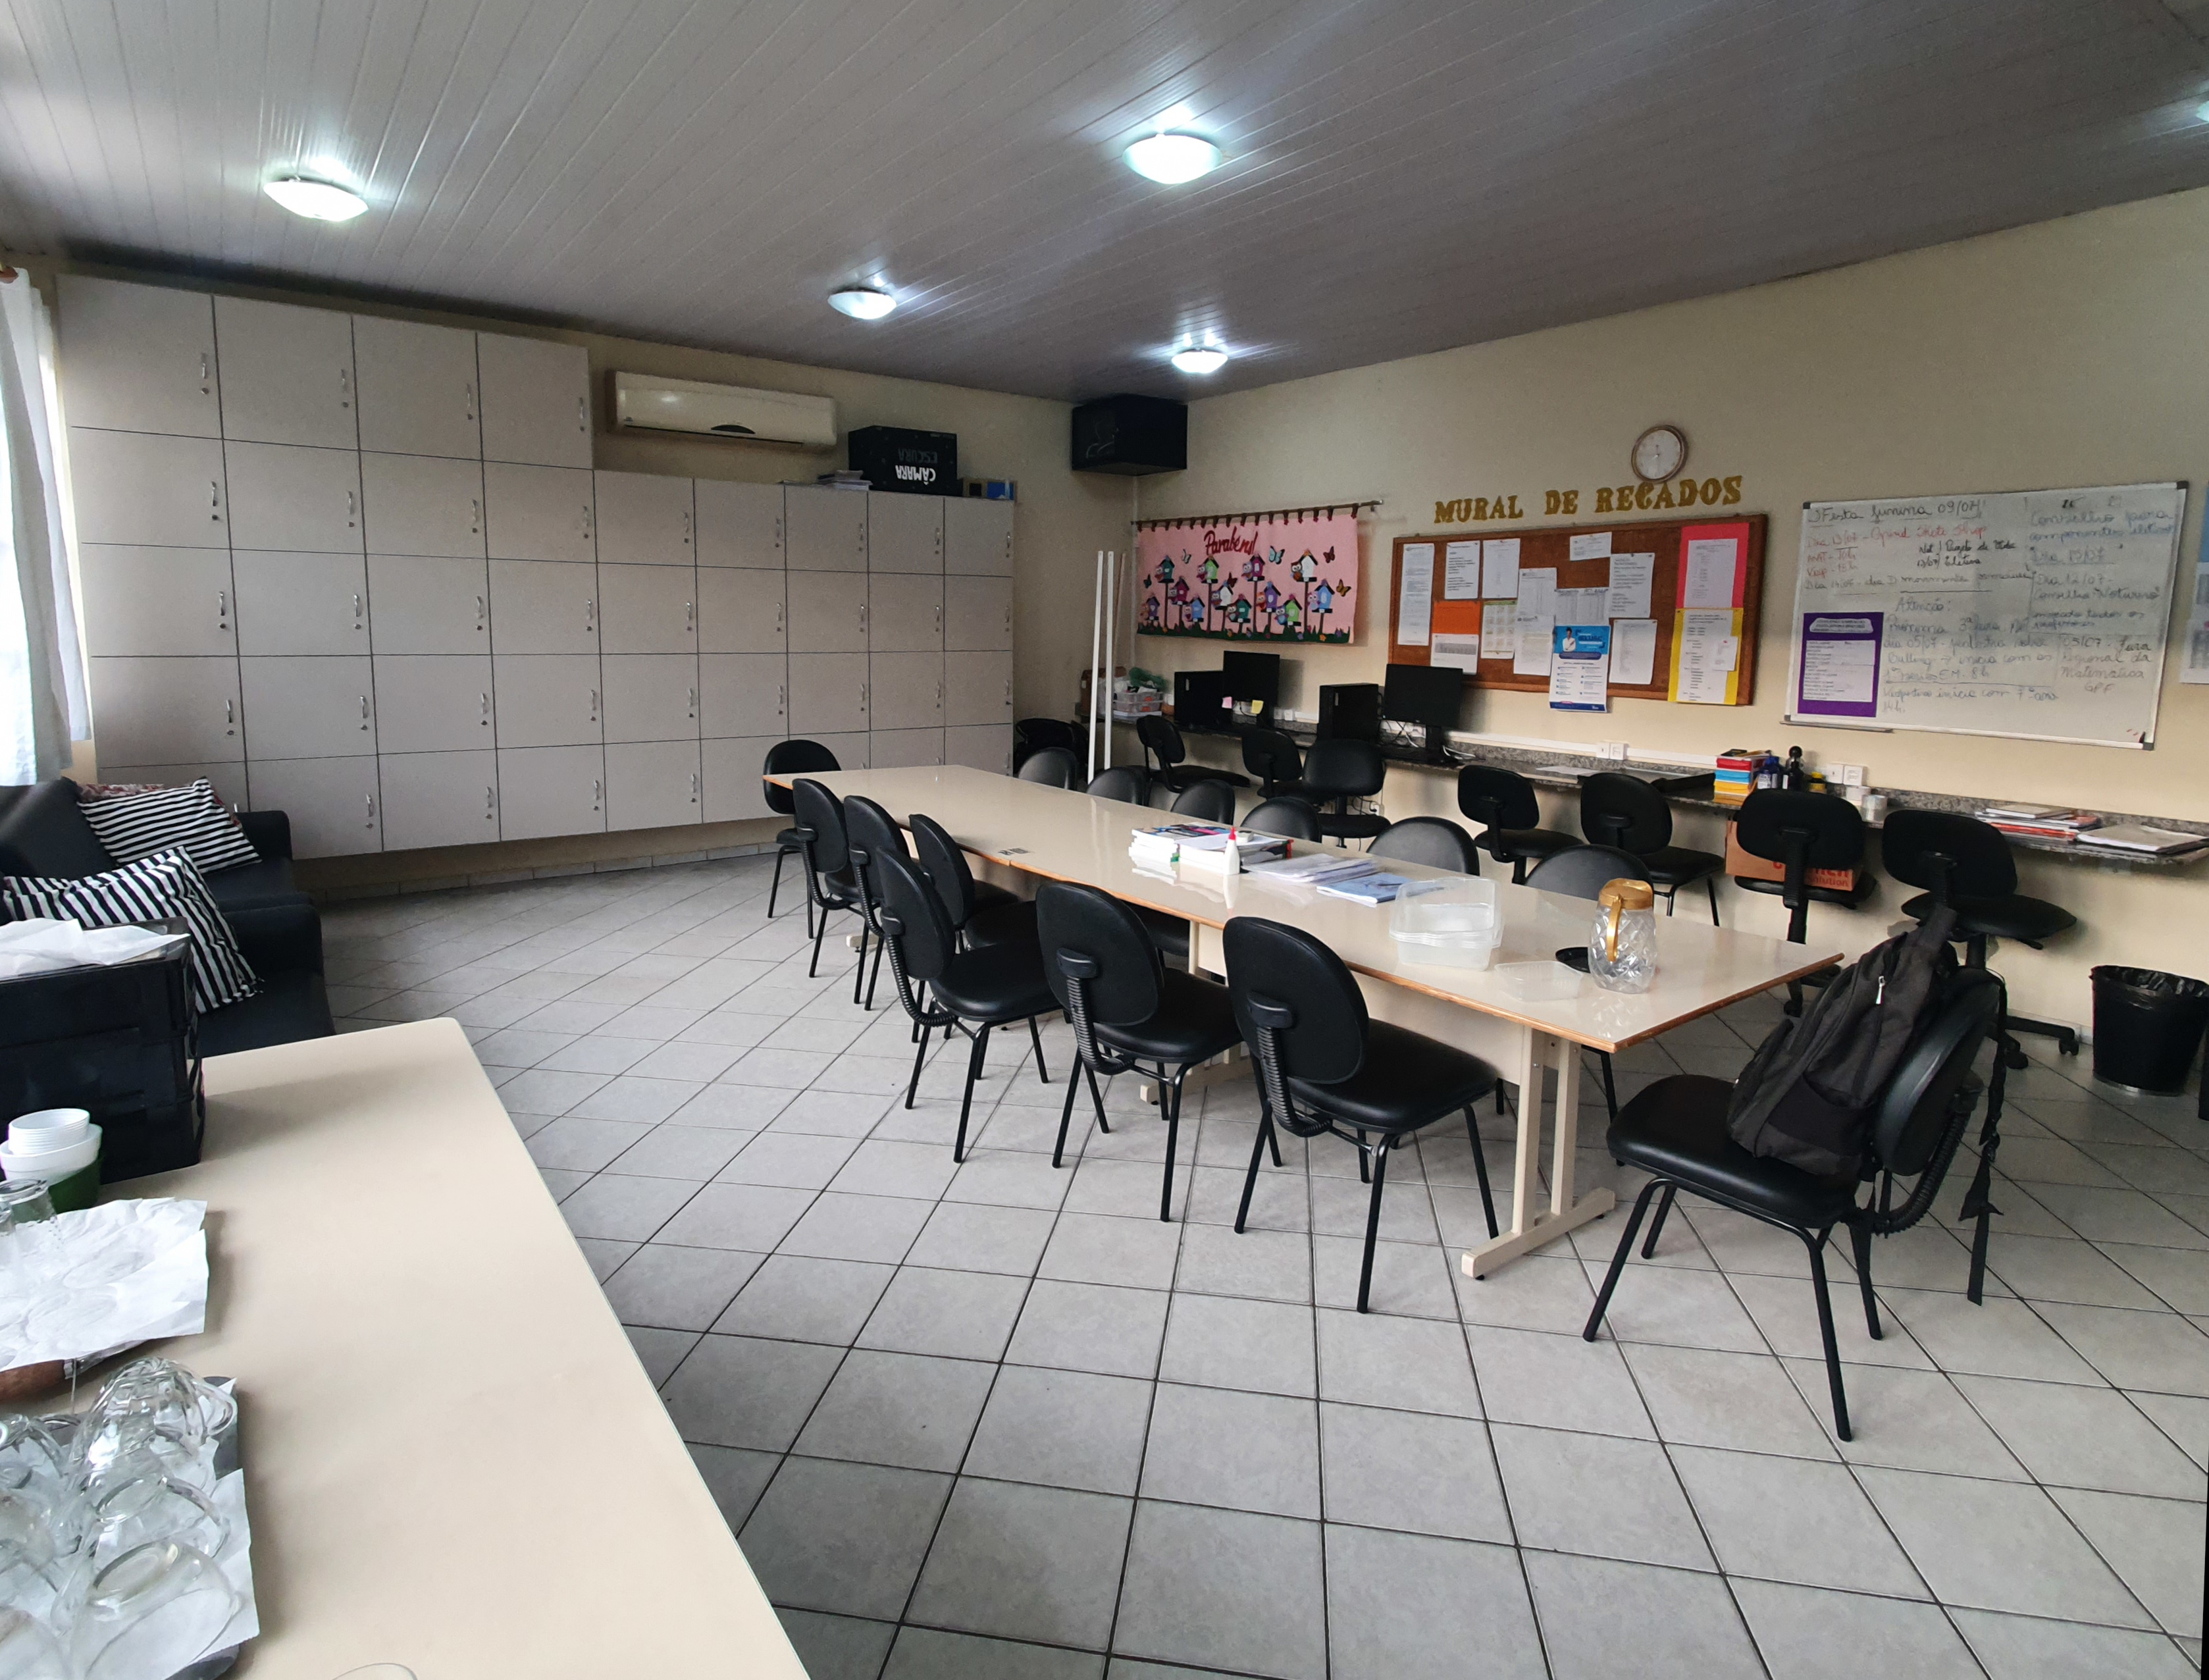
\includegraphics[width=.45\textwidth]{03-elementos/03.2_textual/03.2.1_fig/sala-de-profs01.jpg}
    \caption{Sala dos Professores}
    \label{fig:salaDosProfs}
\end{wrapfigure}
Bem espaçosa a Sala dos Professores, \autoref{fig:salaDosProfs}, possui: geladeira, forno de micro-ondas, aparelho de ar-condicionado e um purificador de água. É equipada com dois desktops conectados à internet. Cada professor tem um espaço nos armários e é nele que fica guardado o \emph{Data-Show} para uso em aulas diferenciadas.

\section{Laboratório}
As aulas experimentais podem ser conduzidas no Laboratório, preparado para atender as disciplinas de Física, Química e Biologia. Comporta cerca de 40 alunos e é composto por duas grandes bancadas e alguns armários. Há nele alguns materiais para conduzir experimentos de cinemática, física térmica e eletrostática, no entanto o professor da disciplina prefere usar a sala de aula para estas atividades.

\section{Laboratório de informática}
\setlength\intextsep{0pt}
\begin{wrapfigure}[7]{l}{0.45\textwidth}
    \centering
    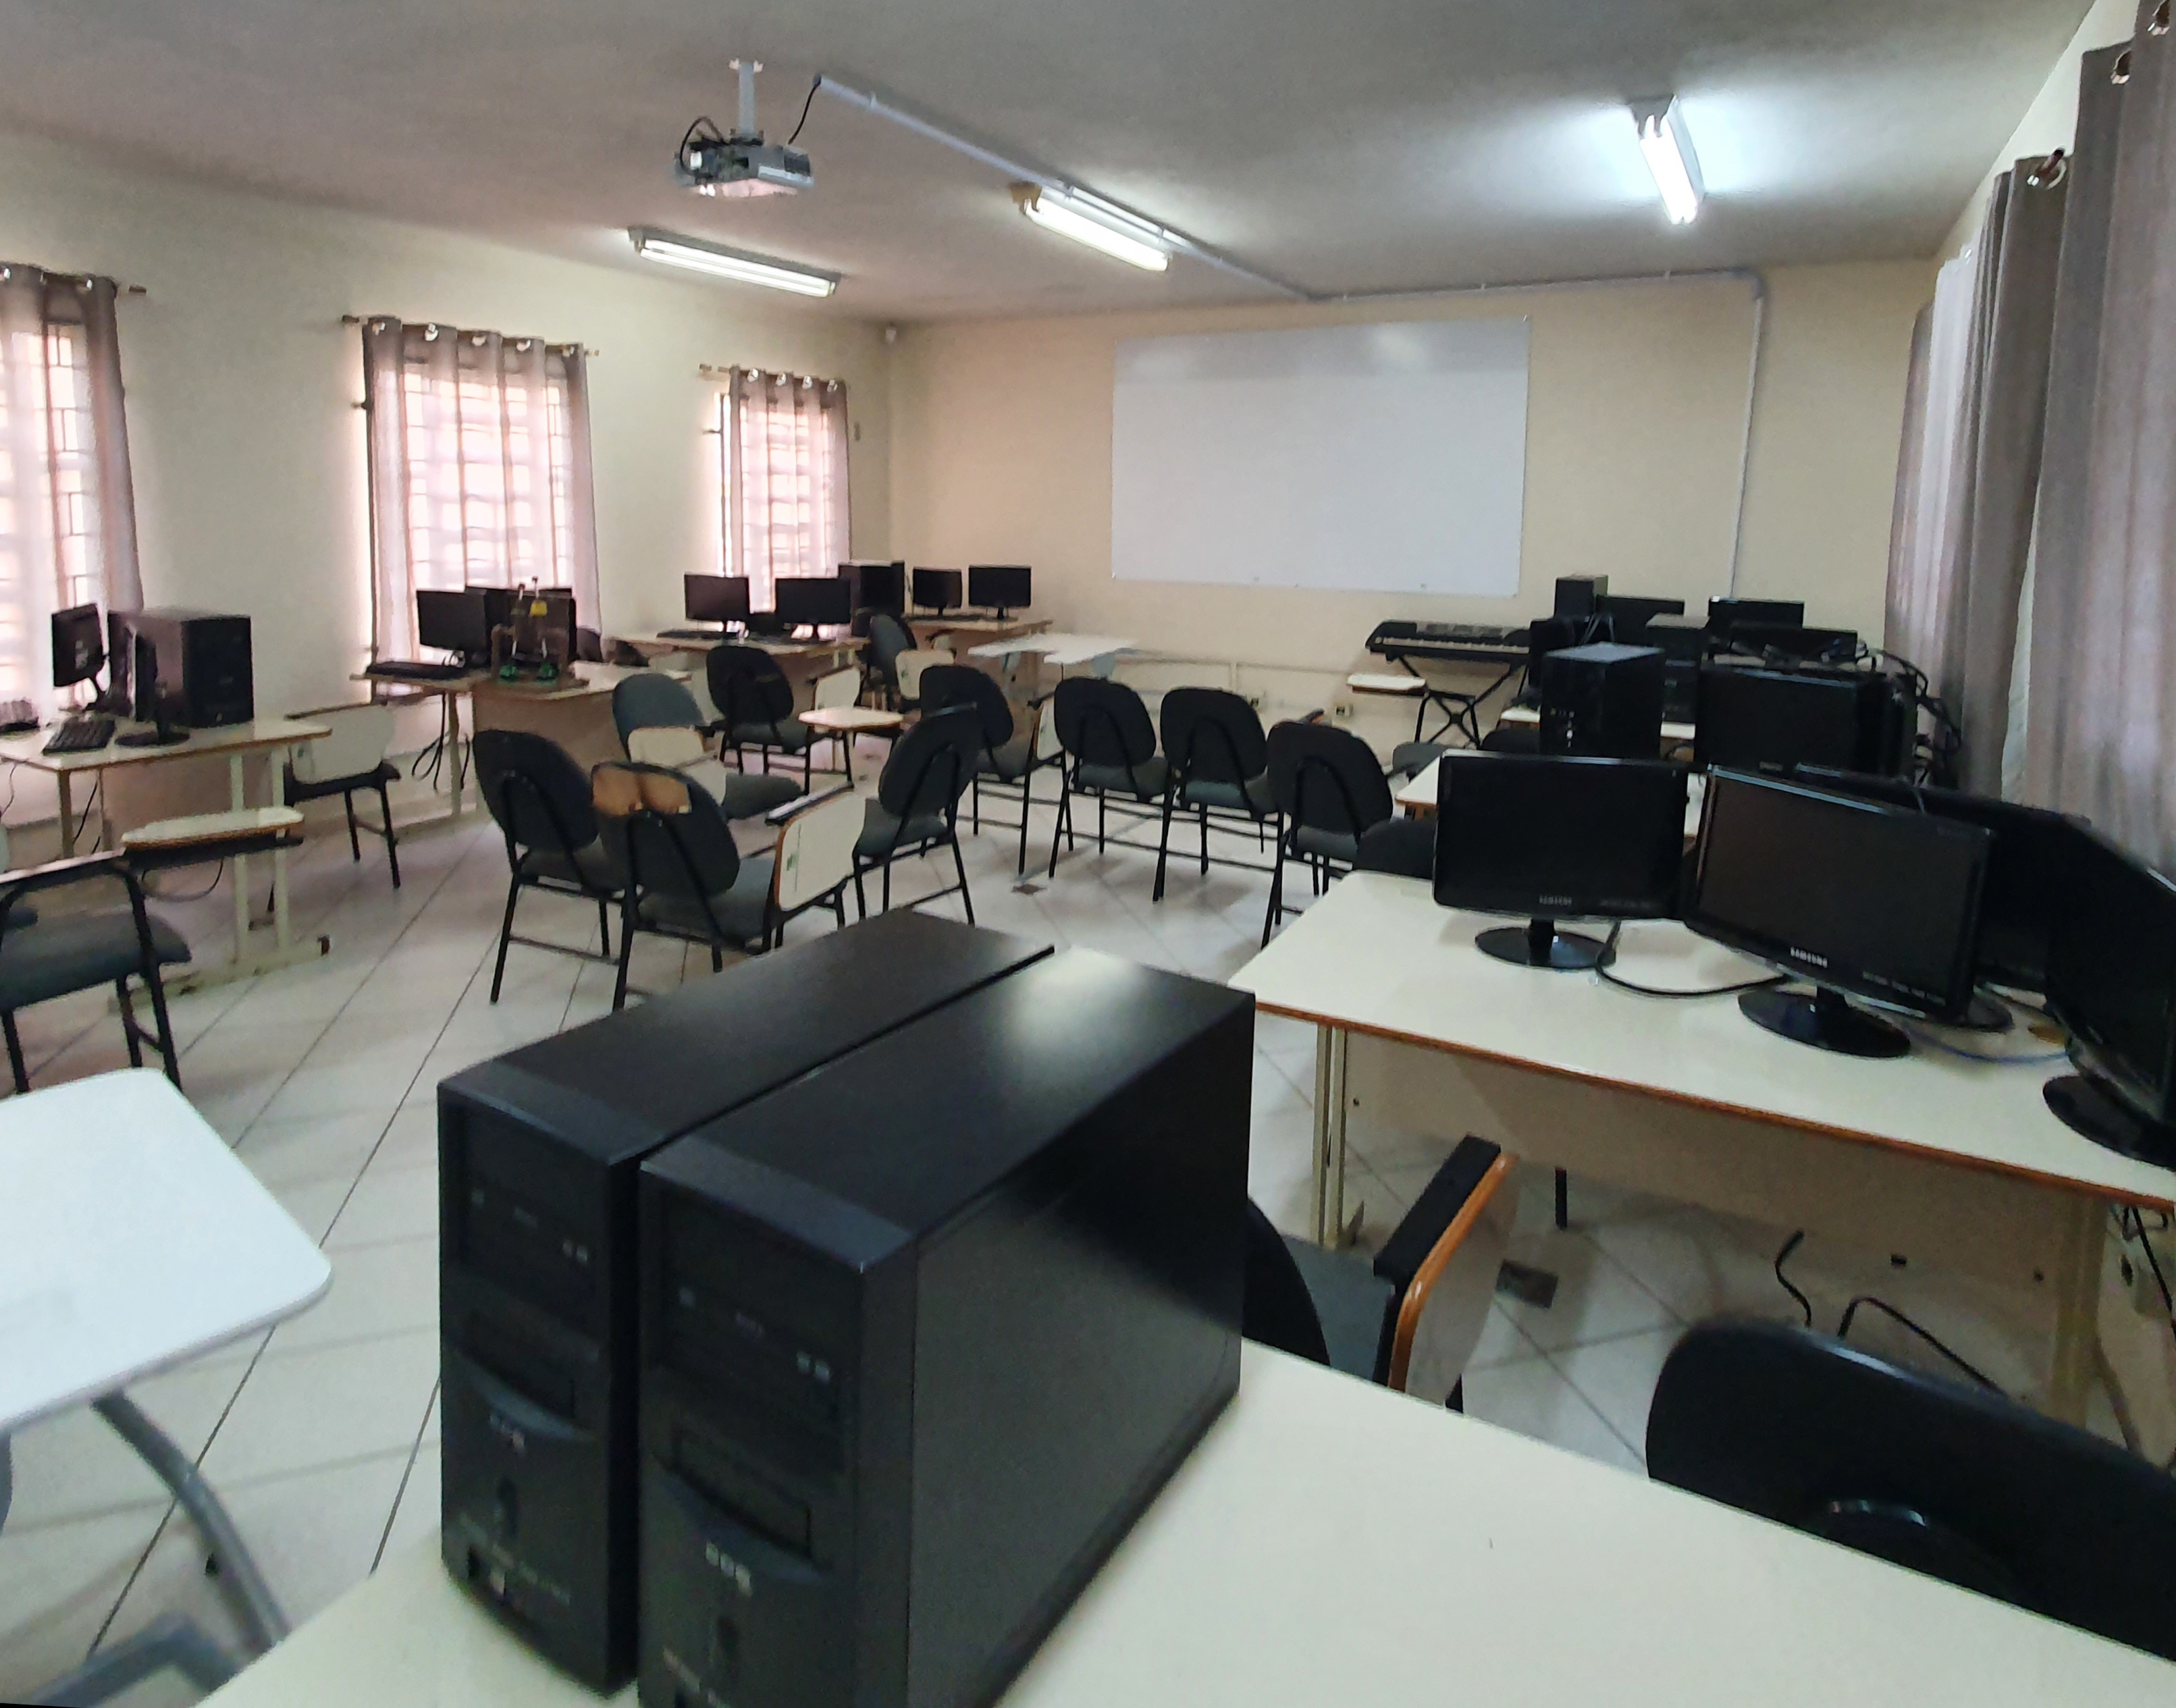
\includegraphics[width=.4\textwidth]{03-elementos/03.2_textual/03.2.1_fig/sala-de-informatica02.jpg} 
    \caption{Laboratório de informática}
    \label{fig:salaDeInformatica}  
\end{wrapfigure}
O Laboratório de Informática, \autoref{fig:salaDeInformatica}, é composto por nove desktops e dezenove monitores com acesso à internet, tem capacidade para atender até dezenove alunos em virtude da quantidade de dispositivos. Possui ainda uma Lousa Melamínica ($350\times 120$)\cm\; e retroprojetor.

\section{Salas de aula}
As Salas de Aulas são planejadas para comportar, em média, trinta alunos. Boa parte das salas possui aparelho de ar-condicionado, armários e são devidamente equipadas com Lousa Melamínica ($400\times 120$)\cm.

\section{Auditório}
\setlength\intextsep{0pt}
\begin{wrapfigure}[9]{r}{0.4\linewidth}
    \centering
    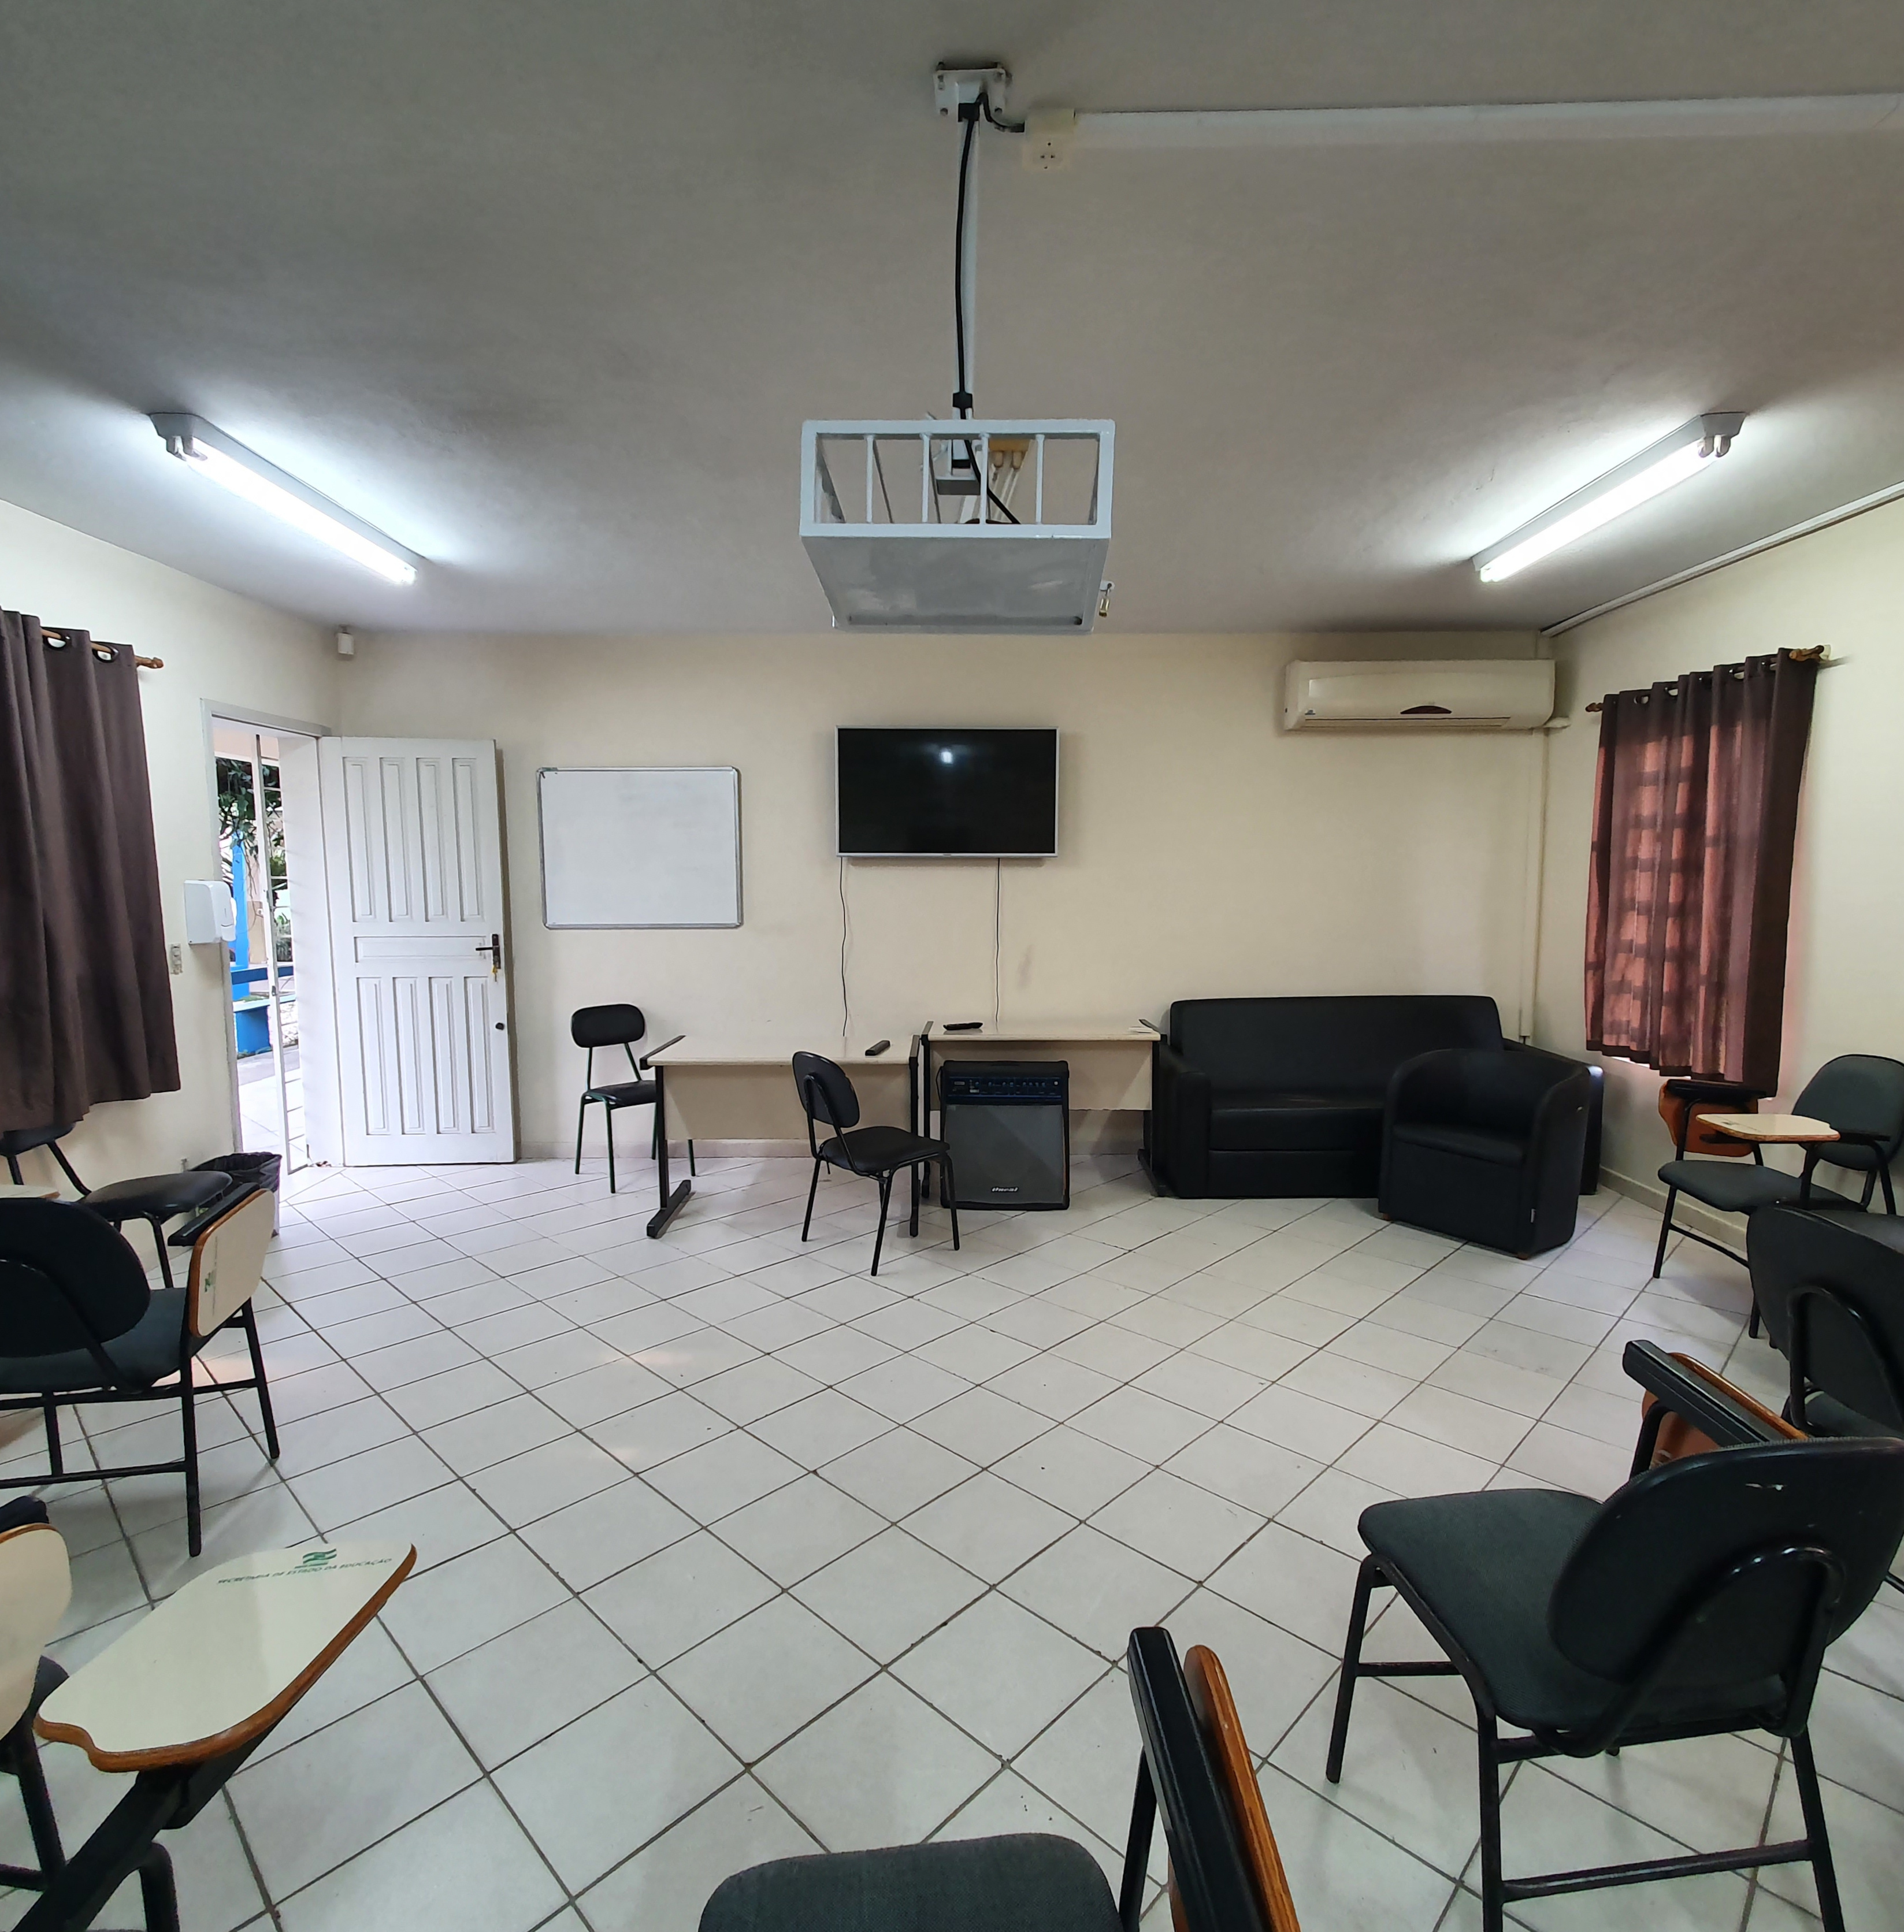
\includegraphics[width=.35\textwidth]{03-elementos/03.2_textual/03.2.1_fig/auditorio01.jpg} 
    \caption{Auditório}
    \label{fig:auditorio}    
\end{wrapfigure}
O auditório, \autoref{fig:auditorio}, tem capacidade para comportar um total quarenta pessoas e é equipado com um televisor de led $40\inch$, caixa de som amplificada multi-uso Oneal-OCM modelo 550 de $80\Watt$ de potência rms, um retroprojetor e ar-condicionado.

\section{Biblioteca}
No acervo da Biblioteca, \autoref{fig:biblioteca}, encontram-se livros didáticos de todas as disciplinas, livros de literatura nacional e internacional, almanaques, \acp{DVD} educativos, revistas de assuntos dos mais variados e jornais. Possui também uma televisão de $32\inch$ a tubo conectada à uma leitora de \ac{DVD}, mesas e cadeiras o suficiente para comportar uma pequena turma de 10 pessoas.
\vspace{8pt}

\begin{figure}[!ht]
    \begin{center}
        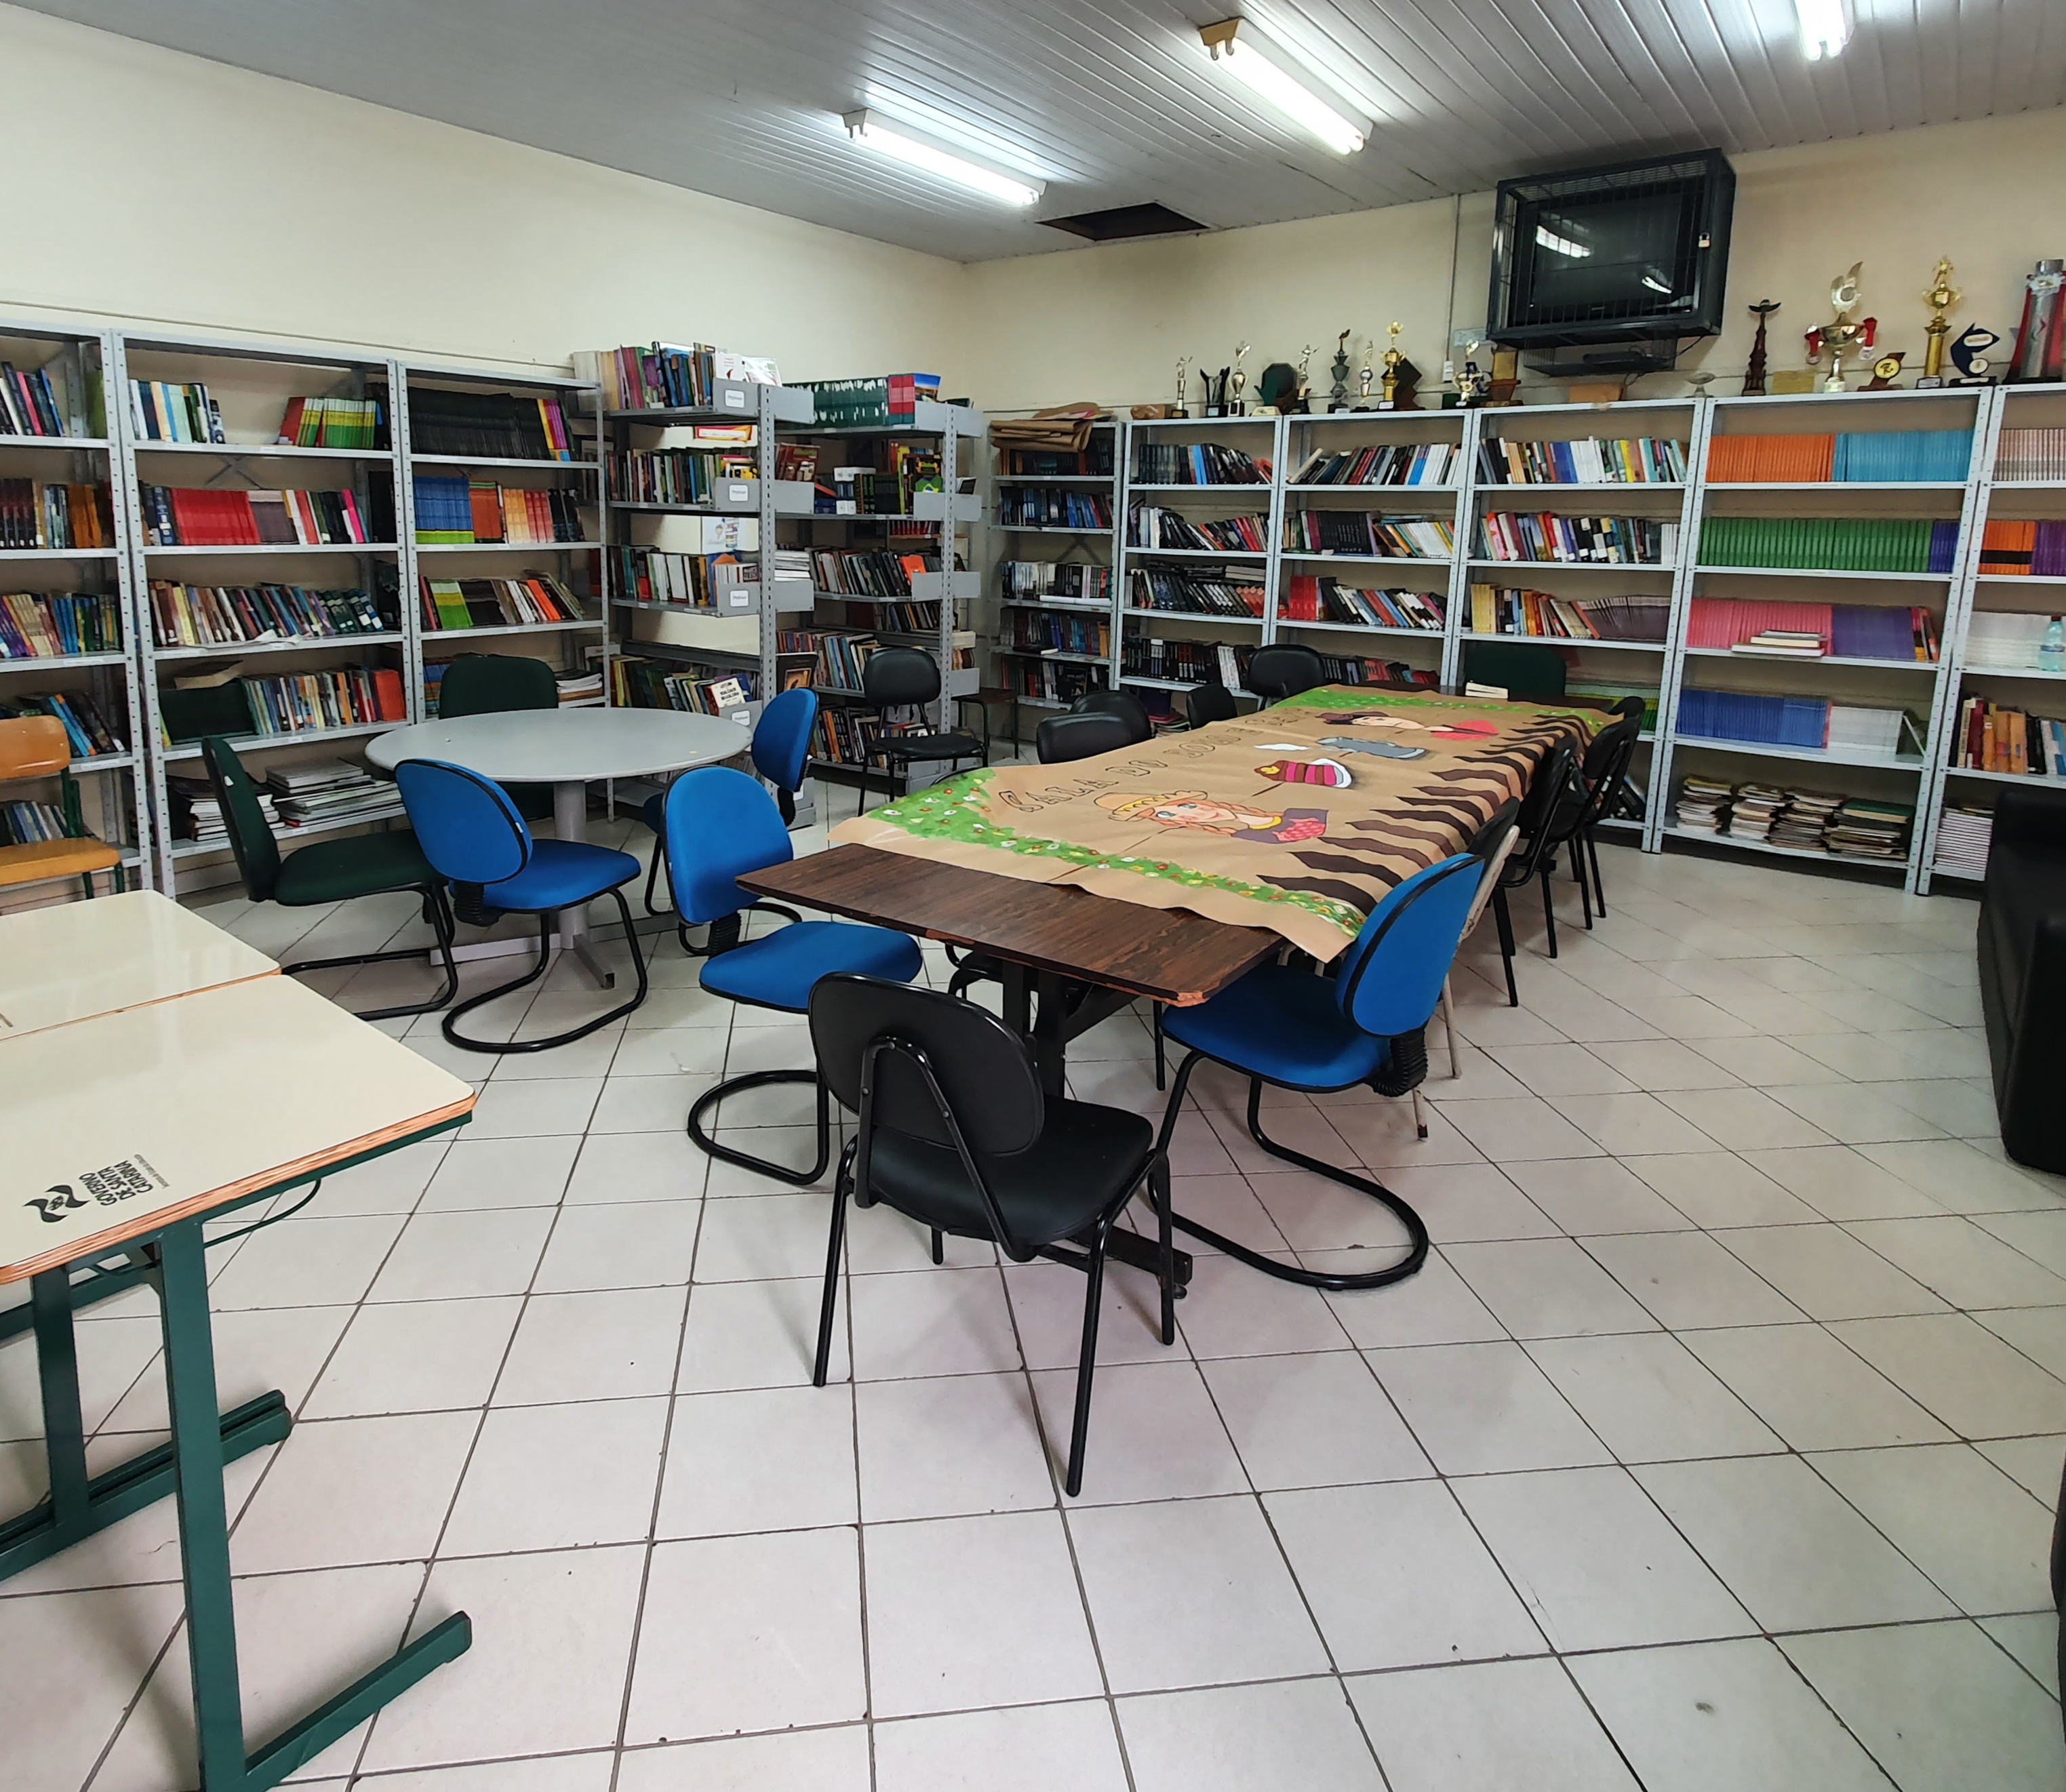
\includegraphics[width=.6\textwidth]{03-elementos/03.2_textual/03.2.1_fig/biblioteca01.jpg}
        \caption{Biblioteca}
        \label{fig:biblioteca} 
    \end{center}    
\end{figure}

%\newpage
\section{Outros Recursos}
\setlength\intextsep{0pt}
\begin{wrapfigure}[11]{l}{0.5\linewidth}
    \centering
    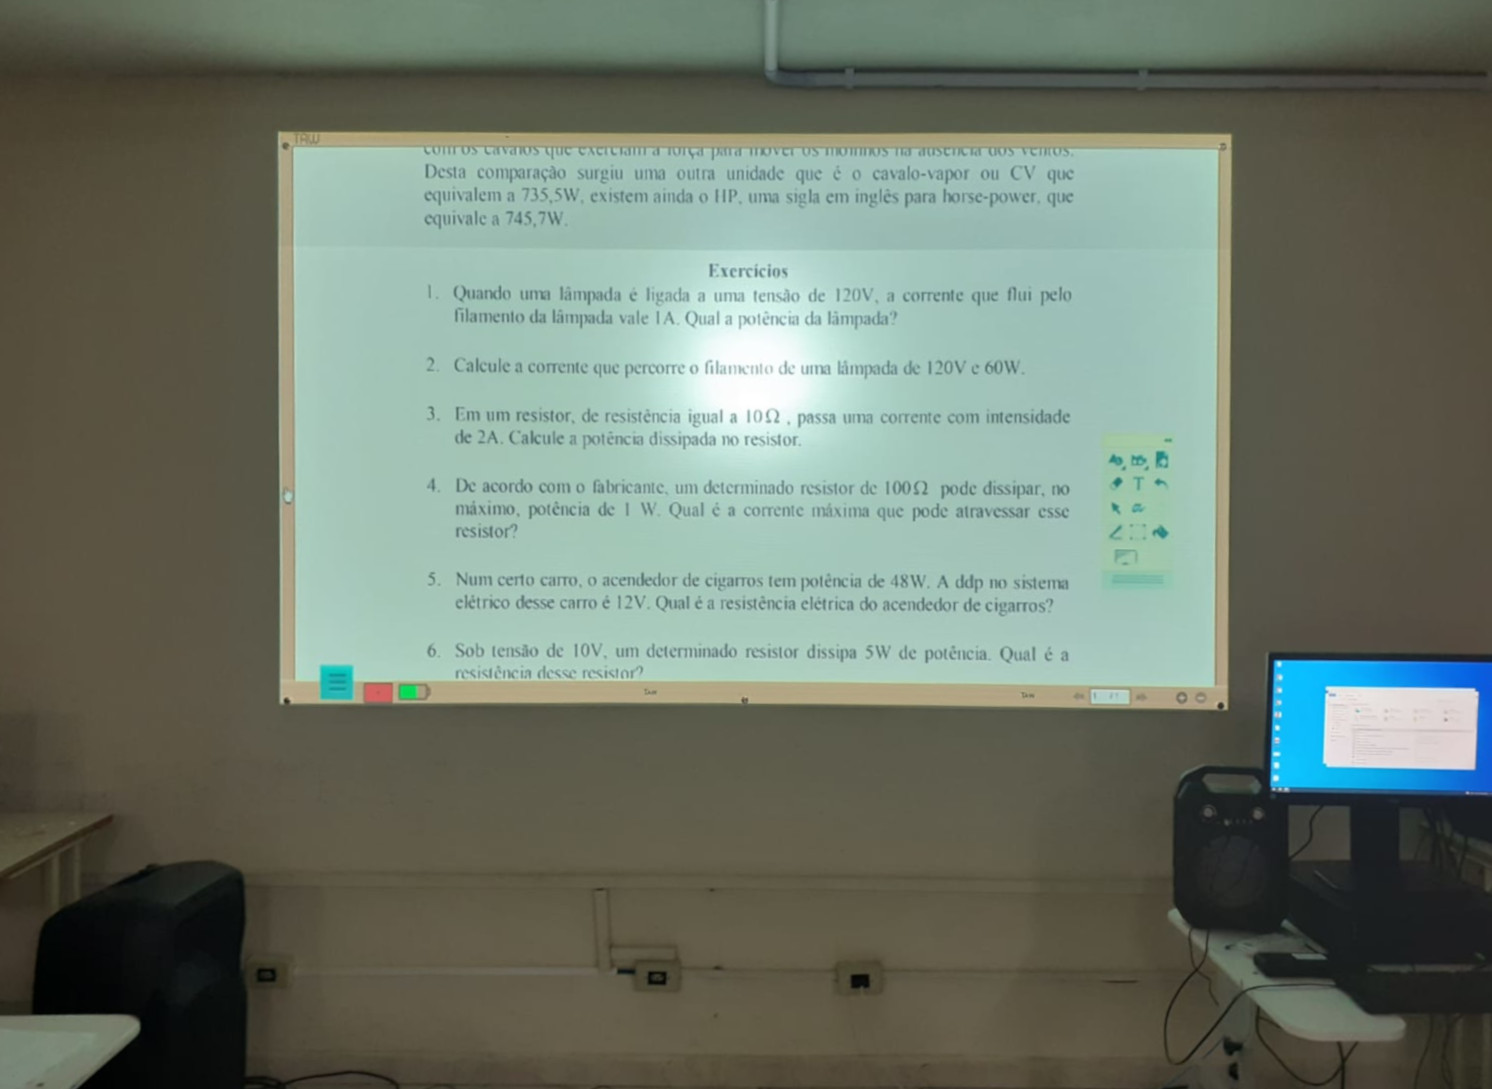
\includegraphics[width=.45\textwidth]{03-elementos/03.2_textual/03.2.1_fig/d-lousa.jpeg} 
    \caption{Lousa Digital}
    \label{fig:lousa-d}    
\end{wrapfigure}
Recentemente foi instalada uma lousa digital interativa em apenas uma sala de aula, \autoref{fig:lousa-d}, nela é possível mostrar simulações, vídeos, sons, GIFs etc. É um recurso que poucos professores utilizam no momento, por somente haver uma em toda a escola. A escola tem previsão de até o final do ano de 2023, todas as salas de aulas possuam o equipamento instalado. A lousa já possui todos os dispositivos necessários para o seu devido funcionamento, ficando a critério do professor a opção de levar ou não seu notebook ou que mais achar melhor para incrementar a aula.

\section{Tablets}
A unidade também possui 32 Tablets conectados à internet de 200 Mb e com o sistema operacional Android. Neles, o professor costuma usar o aplicativo \emph{Kahoot} em atividades diferenciadas. Para manter os tablets sempre com a bateria carregadas e prontos para uso, a escola utiliza o gabinete móvel de recarga, como pode ser visto na \autoref{fig:tablets}.
\begin{figure}[!ht]
\vspace{8pt}
    \begin{center}
        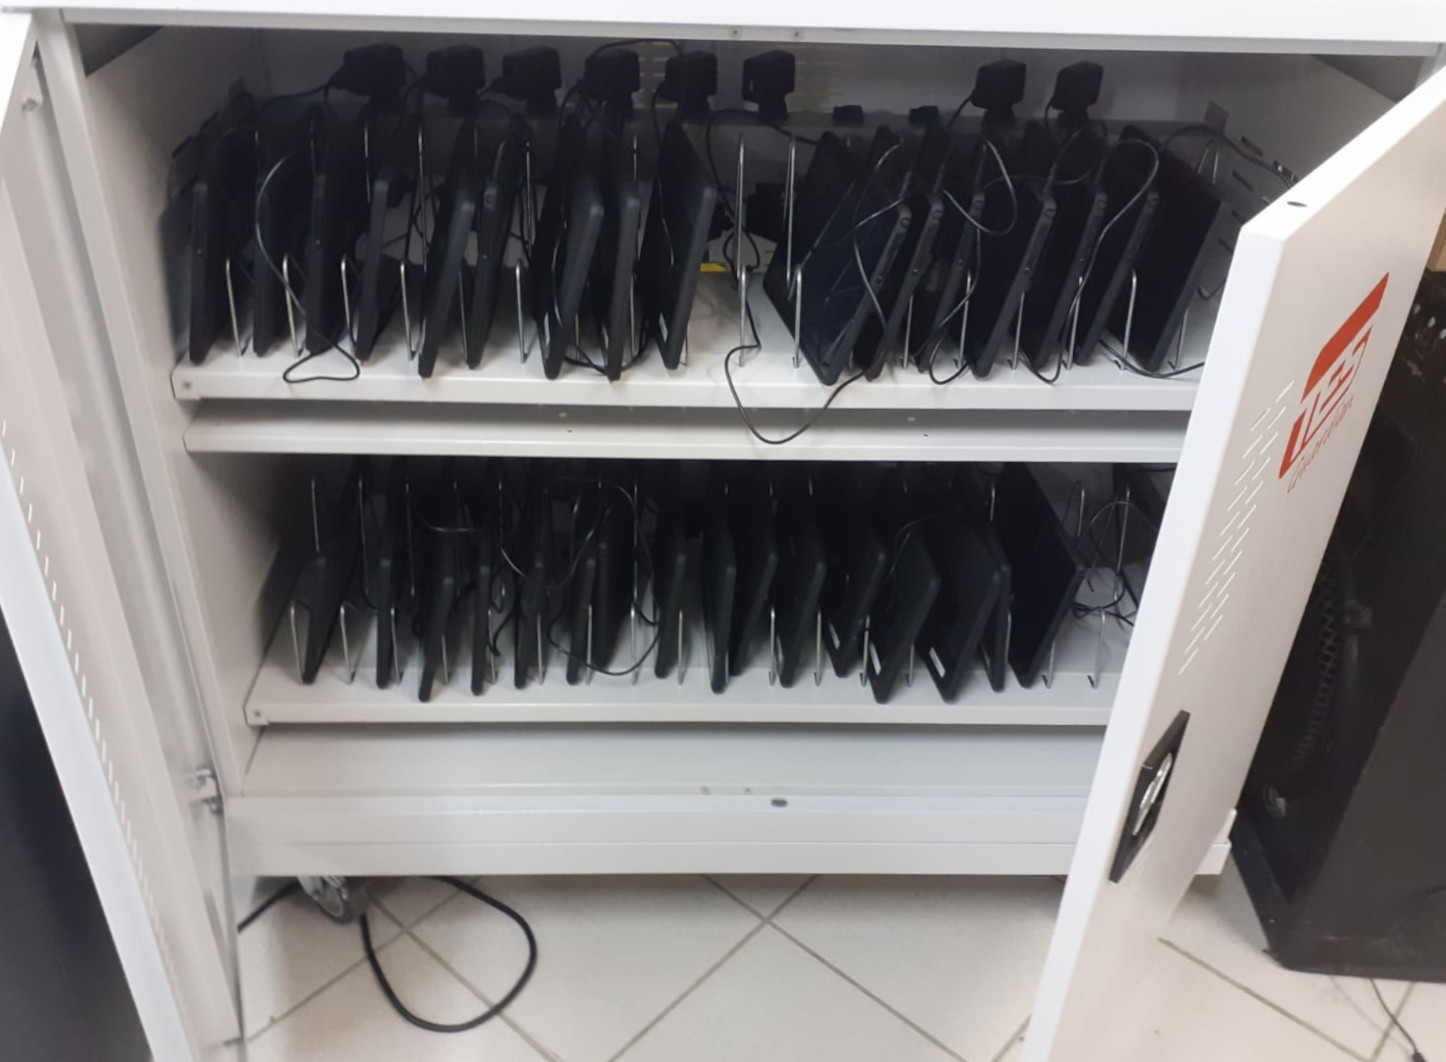
\includegraphics[width=.8\textwidth]{03-elementos/03.2_textual/03.2.1_fig/tablets.jpeg} 
        \caption{Tablets}
        \label{fig:tablets}    
    \end{center}
\end{figure}

\chapter{Programas de Física para o Ensino Médio}
\thispagestyle{empty}
\label{cap: prgFisica}
O acesso ao Planejamento Anual do Professor Supervisor não foi viabilizado neste estágio, de modo que a análise que aqui se estende, tem por base os materiais disponibilizados às turmas de segundo e terceiro ano, no ambiente virtual \emph{Google Classroom}. Nesta análise, não se inclui os primeiros anos em virtude de que o Professor Supervisor não as atendia no momento em que foi escrito este relatório.

\section{Conteúdos Abordados nos Segundos Anos}
A \autoref{fig:classroomSegundoAno} mostra os últimos conteúdos de Física do segundo ano lecionados até o mês de setembro do ano de 2022. Nela podemos ver uma estrutura de tópicos inseridos à medida que o professor vai avançando na disciplina.
\vspace{.5cm} 
\begin{figure}[!htpb]
    \begin{center}
        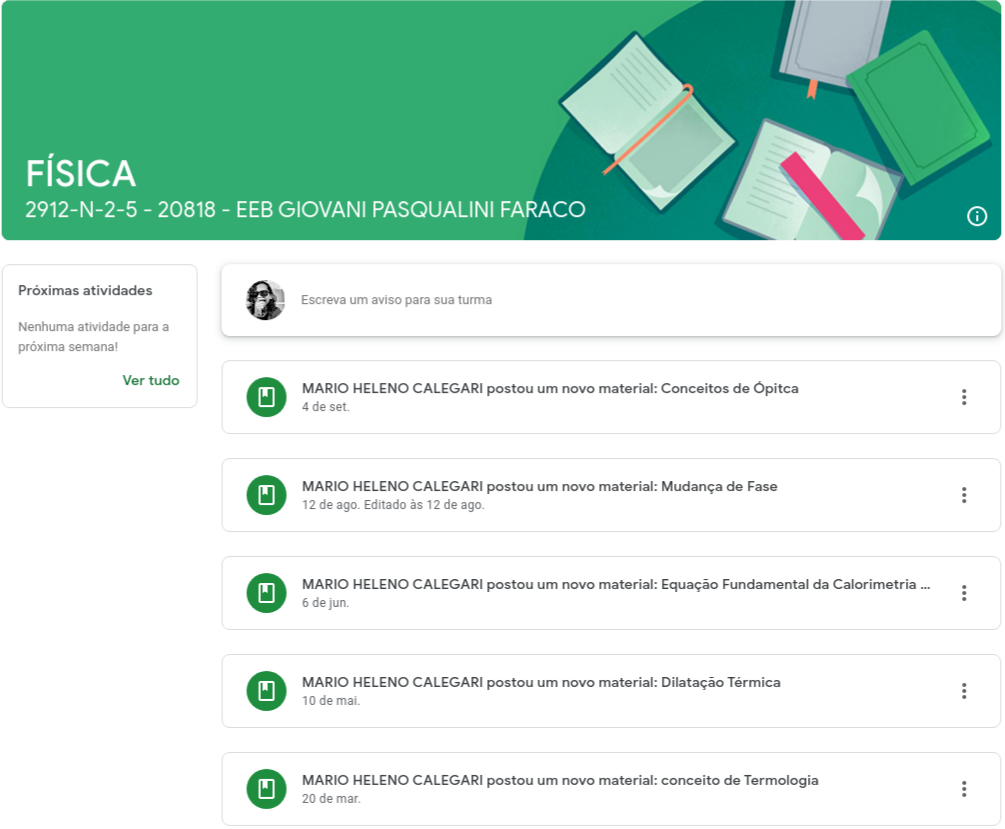
\includegraphics[width=.95\textwidth]{03-elementos/03.2_textual/03.2.1_fig/programaFisica2-5.png}
        \caption{Conteúdos de Física 2°(5) -- Google Classroom}
        \label{fig:classroomSegundoAno}
    \end{center}    
\end{figure}

Esta unidade trata essencialmente dos assuntos relacionados à Energia. A sequência completa até o momento é apresentada como segue: \emph{1. Energia Mecânica, 2. Termologia, 3. Dilatação Térmica, 4. Equação Fundamental da Calorimetria, 5. Mudança de Fase e 6. Conceitos de Óptica.}

Assim disposto, vemos que a sequência segue ainda a forma apresentada tradicionalmente nos livros didáticos da disciplina, com exceção do tópico Energia Mecânica, o qual normalmente é tratado ao final do primeiro ano do Ensino Médio. As seções internas de cada tópico apresentado no Google Classrom segue a seguinte abordagem: apresentação dos conceitos/teorias, seguido de alguns exemplos de substituição direta e finalizando com uma lista de exercícios. Para melhor compreensão e visualização, um elemento da unidade relacionada a Dilatação Térmica dos materiais pode ser visto na íntegra na \autoref{anx:materialAnexoDilatacaoTermica} do Anexo \ref{anx:materiaisAnexo}.  

Uma das características mais marcantes da \ac{BNCC}, diz respeito à \emph{flexibilização dos currículos}. O atendimento a este princípio exige que \emph{``[\ldots] se rompa com a centralidade das disciplinas, em prol de um currículo que contemple a complexidade das relações existentes entre os ramos da ciência''} \cite{BRASIL:2017}. Além disso, deve-se estimular continuamente o protagonismo dos estudantes, de forma que

\begin{citacao}
    ``evidencie a contextualização, a diversificação e a transdisciplinaridade ou outras formas de interação e articulação entre diferentes campos de saberes específicos, contemplando vivências práticas e vinculando a educação escolar ao mundo do trabalho e à prática social e possibilitando o aproveitamento de estudos e o reconhecimento de saberes adquiridos nas experiências pessoais, sociais e do trabalho.'' \cite{BRASIL:2018}
\end{citacao}
Neste sentido entende-se que não só a predisposição, como até mesmo os próprios assuntos ofertados, ao atender aos pressupostos da Base, devam ser capazes de promover um diálogo constante com as realidades locais de cada unidade escolar. Da forma como é estabelecida, estas exigências não privilegiam uma sequência em detrimento da outra, apenas atentam sobre as particularidades a que cada contexto e/ou grupo escolar esteja imerso em sua realidade de ensino, desde que possibilite o protagonismo dos estudantes, de modo a proporcionar o pensamento crítico perante as questões da contemporaneidade.

Já a \ac{PCSC} trata o tema Energia como objeto de estudo designado por meio de \emph{conceitos fundantes}, orienta que o ensino de Física deva seguir de forma contextualizada e centrada nestes conceitos de forma dialogada e estimulante \cite[p.~164]{BRASIL:2017}. Estas duas visões não encontram-se dissonantes, mas reforçam-se na concepção de um currículo interdisciplinar, estimulante, contextualizado e dialógico.

Considerando o exposto, vê-se ainda certa resistência à adequação deste currículo, em atenção às novas exigências propostas pelas reformas, ao menos no que tange o planejamento de um currículo contextualizado, dialógico e próximo à realidade do estudante.

\section{Conteúdos Abordados nos Terceiro Anos}
Seguindo como na seção anterior, tem-se na \autoref{fig:classroomTerceiroAno} a sequência utilizada até o momento, contendo a estrutura dos últimos tópicos das aulas ministradas entre as turmas de terceiro ano.
\vspace{.5cm} 
\begin{figure}[!ht]
    \begin{center}
        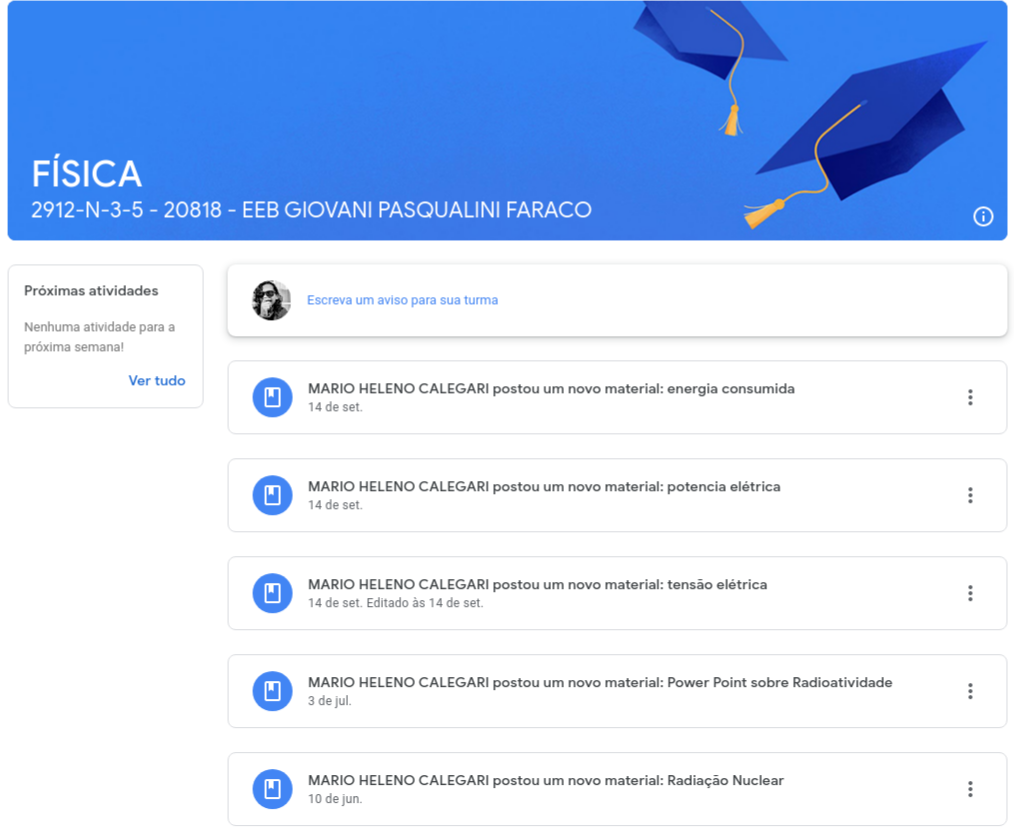
\includegraphics[width=\textwidth]{03-elementos/03.2_textual/03.2.1_fig/programaFisica3-5.png}
        \caption{Conteúdos de Física 3°(5) -- Google Classroom}
        \label{fig:classroomTerceiroAno}
    \end{center}    
\end{figure}

Aqui vemos uma abordagem similar a anterior, seguindo a ordem dos livros didáticos tradicionais: \emph{1. Conceitos de Eletricidade, 2. Lei de Coulomb, 3. Corrente Elétrica, 4. Radiação Nuclear, 5. Radioatividade, 6. Tensão Elétrica, 7. Potência Elétrica e 8. Energia Consumida}. A inserção dos tópicos relacionados à \emph{Radiação e Radioatividade} quebra a estrutura tradicional dos livros, uma vez que este assunto é visto (quando visto), em tópicos mais avançados, junto com ondas eletromagnéticas e/ou estrutura da matéria.

A metodologia utilizada, mais especificamente no tópico relacionado à Radioatividade, aborda o assunto do ponto de vista da História da Ciência -- \emph{História da Radiação}, precisamente. A abordagem desdobra-se, dentre outras formas, trazendo o contexto das descobertas científicas da época para dentro da sala de aula, atendendo a algumas das exigências da \ac{PCSC} como, por exemplo:

\begin{citacao}
    ``O aprofundamento na formação científica envolve a caracterização dos elementos químicos partindo de suas propriedades, seguindo-se de sua representação e modelagem, \ldots enfocando a evolução dos modelos atômicos, incluindo modelos quânticos que permitem a compreensão da tabela periódica dos elementos. Ao mesmo tempo, se reconhece e apresenta a ciência como uma construção humana, associada ao desenvolvimento produtivo, buscando assim enfatizar a presença das tecnologias em todos os períodos da história econômica e em todos os setores da vida.'' \opcit[p.~169--170]{PCSC:2014}
\end{citacao}
Sendo assim, configura-se aqui uma tímida aproximação deste currículo com a Proposta de Santa Catarina, capaz de contribuir para a formação do pensamento crítico e autonomia de pensamento, por meio da reflexão à cerca do desenvolvimento da ciência como atividade humana sujeita aos paradigmas de sua época.

\chapter{Acompanhamento de Aulas}
\thispagestyle{empty}
\label{cap:acompanhamento-de-aulas}

Um total de 12 aulas foram assistidas subdivididas em 03 turmas; uma do segundo ano e outras duas do terceiro ano. Os conteúdos abordados encontram-se elencados no \autoref{qua:acompanhamento de aulas}:

\vspace{10pt}
\begin{quadro}[!ht]
\centering
\resizebox{\textwidth}{!}{%
\begin{tabular}{|c|c|c|c|l|}
\hline
\multicolumn{1}{|l|}{\textbf{Aula}} &
  \multicolumn{1}{l|}{\textbf{Dia}} &
  \multicolumn{1}{l|}{\textbf{Período}} &
  \multicolumn{1}{l|}{\textbf{Turma}} &
  \textbf{Conteúdos Abordados} \\ \hline
01 & \multirow{5}{*}{16/09} & \multirow{12}{*}{Noturno} & 3º(4) & Energia Consumida                 \\ \cline{1-1} \cline{4-5} 
02 &                        &                           & 3º(5) & Energia Consumida                 \\ \cline{1-1} \cline{4-5} 
03 &                        &                           & 2º(5) & Conceitos de Óptica Geométrica    \\ \cline{1-1} \cline{4-5} 
04 &                        &                           & 2º(5) & Proposta de Atividade             \\ \cline{1-1} \cline{4-5} 
05 &                        &                           & 3º(4) & Energia Consumida                 \\ \cline{1-2} \cline{4-5} 
06 & \multirow{5}{*}{30/09} &                           & 3º(4) & Energia Consumida                 \\ \cline{1-1} \cline{4-5} 
07 &                        &                           & 3º(5) & Energia Consumida                 \\ \cline{1-1} \cline{4-5} 
08 &                        &                           & 2º(5) & Apresentação de Atividade         \\ \cline{1-1} \cline{4-5} 
09 &                        &                           & 2º(5) & Apresentação de Atividade         \\ \cline{1-1} \cline{4-5} 
10 &                        &                           & 3º(4) & Energia Consumida                 \\ \cline{1-2} \cline{4-5} 
11 & \multirow{2}{*}{25/11} &                           & 2º(5) & O Experimento de Michelson-Morley \\ \cline{1-1} \cline{4-5} 
12 &                        &                           & 2º(5) & As Transformações de Lorentz      \\ \hline
\end{tabular}%
}
\caption{Cronograma de aulas assistidas}
\label{qua:acompanhamento de aulas}
\end{quadro}
\vspace{10pt}

Foi possível identificar três tipos de abordagens, sendo estas classificadas como: \emph{atividade investigativa; aulas de introdução de conteúdo e aulas de exercícios.} A seguir será feita a análise destas abordagens.

\section{Abordagens Relacionadas à Introdução de Conteúdo}
Nesta abordagem o professor frequentemente inicia um conteúdo novo trazendo situações do cotidiano que fazem parte do universo do aluno, por exemplo: Ao introduzir o conceito de \emph{potencia elétrica}, o faz primeiramente dando a definição de potência
\begin{center}
    \begin{minipage}{0.7\textwidth}
        \begin{itemize}
            \item[\textbf{Prof.:}] Potência é [\ldots] a rapidez com que um trabalho é realizado, ou seja, é a medida do trabalho realizado por uma unidade de tempo.
        \end{itemize}
    \end{minipage}
\end{center}
e exemplifica logo na sequência
\begin{center}
    \begin{minipage}{0.7\textwidth}
        \begin{itemize}
            \item[\textbf{Prof.:}] Por exemplo, todos aqui já viram um Fiat Mobi certo? Também sabem o que é um Camaro correto?
            \item[\textbf{Alunos:}] Sim
            \item[\textbf{Prof.:}] Beleza... Entre um Mobi e um Camaro, qual dos dois chega primeiro numa distância, sei lá, daqui até a praia?
            \item[\textbf{Alunos:}] O Camaro né professor!
        \end{itemize}
    \end{minipage}
\end{center}
De acordo com \cite{Carvalho1999} esta estratégia visa aproximar os conceitos representativos da unidade de ensino, ao universo sensível dos estudantes, e é capaz de promover uma passagem da linguagem coloquial para a linguagem científica de forma natural.

Também é possível notar a gênese da formação dos padrões de interação oriundos da dinâmica que vai se construindo em sala de aula conforme discutido por \cite{MORTIMER2002}. Tais padrões se complexificam a medida que professor e alunos vão avançando no decorrer das exposição, como pode visto na passagem a seguir:

\begin{center}
    \begin{minipage}{0.7\textwidth}
    \begin{itemize} 
        \item[\textbf{A[1]:}] \ldots então quer dizer que ele [o Camaro] tem a força de 400 cavalo professor?        
        \item[\textbf{A[2]:}] Meu já pensou, tipo o carro é uma fazenda de cavalo [Risos]
        \item[\textbf{Prof.:}] Tem que ver qual que é força do cavalo
        \item[\textbf{A[1]:}] Não sei
        \item[\textbf{Prof.:}] Nós já vamos ver quanto que vale essa unidade [cavalo-vapor], se vocês quiserem pesquisem ai quanto que um cavalo faz de força
    \end{itemize}        
    \end{minipage}
\end{center}
Esta dinâmica permite a formação das tríades I-R-F a medida que o professor promove a discussão em sala e mantém ativa a fala dos estudantes, retroalimentando o ciclo a cada nova interação.

Este padrão foi observado com menos intensidade na aula 03 em que o professor introduzia os conceitos de óptica geométrica por meio de uma sequência de slides, na ocasião o professor trouxe o exemplo da câmara escura por meio de um vídeo, e fazia questões como

\begin{center}
    \begin{minipage}{0.7\textwidth}
        \begin{itemize}
            \item[\textbf{Prof.:}] Todo mundo aqui já viu uma câmera fotográfica?
            \item[\textbf{Prof.:}] Como vocês imaginam que funciona uma câmera?
            \item[\textbf{A[1]:}] A luz passa pela lente
            \item[\textbf{Prof.:}] Ta, passa pela lente e aí acontece alguma coisa
        \end{itemize}
    \end{minipage}
\end{center}

 Neste episódio as respostas eram mais tímidas e diretas, a abordagem comunicativa não evoluiu para padrões mais complexos. Estima-se que pela complexidade do assunto, os alunos tenham se sentido menos a vontade. Ao final o professor propôs uma atividade investigativa visando a construção de uma câmara escura, falaremos um pouco mais desta atividade na sequência.

 \section{Atividade Investigativa}
 Imediatamente após a aula de introdução do conteúdo relacionado aos \emph{Princípio da Óptica Geométrica}, o professor propôs como atividade investigativa, que os alunos pesquisassem e construíssem uma câmara escura, tiveram 20 dias para completar a tarefa e puderam utilizar o que quisessem de material.

 O professor colocou-se à disposição para orientar no que for necessário.

 Não foi possível acompanhar o desenvolvimento desta atividade uma vez que, trata-se de uma turma ao qual é administrada aulas faixas às sextas-feiras e em decorrência da reunião administrativa marcada para o dia 23/09 e da eleição de primeiro turno para a presidência, marcada para o dia 02/10, houve o interrompimento destas aulas durante as duas sextas-feiras seguintes. Portanto, nos limitaremos a analisar somente os resultados da atividade.

 Embora a sala possua 43 alunos matriculados apenas 44\% comparecem frequentemente às aulas, pelo menos nas sextas-feiras, o que reduz a quantidade efetiva de estudantes para $\sim19$ indivíduos. Estes se dividiram em grupos de 3-4 integrantes, 2 grupos apresentaram seus trabalhos no dia combinado e outros 4 ficaram de entregar na próxima aula. Dos que apresentaram, relataram que pesquisaram na internet vendo vídeos como os do \emph{Manual do Mundo} e não sentiram dificuldades na confecção das câmaras.

 Este tipo de abordagem encontra-se bem fundamentada em \cite{Sasseron2015}, no que se convencionou chamar de \emph{Ensino por Investigação}, tem por característica fundamental o de \emph{``promover o papel ativo do estudante na construção do conhecimento científico'' \Ibidem{Sasseron2015}}. Também está de acordo com as orientações da nova \ac{BNCC} no que tange
 
 \begin{citacao}
     ``\ldots garantir o protagonismo dos estudantes em sua aprendizagem e o desenvolvimento de suas capacidades de abstração, reflexão, interpretação, proposição e ação, essenciais à sua autonomia pessoal, profissional, intelectual e política.'' \cite{BRASIL:2017}
 \end{citacao}

 Ainda assim, notou-se uma certa resistência a adesão da atividade pela turma como um todo, parte desta dificuldade deve justificar-se se considerado for o perfil dos estudantes: alunos quietos; introspectivos; boa parte trabalha durante o dia e estuda a noite e etc.

 \section{Aulas de Exercícios}
 Em todas as aulas deste tipo de abordagem, observou-se o mesmo padrão, o professor indica os exercícios que devem ser entregues e a turma por sua vez limita-se a resolvê-los em duplas, trios e etc. Durante a resolução alguns buscam o auxílio do professor e o mesmo se prontifica a ajudar. A maioria dos alunos resolvem e entregam estes exercícios o que torna a atividade a principal fonte de avaliações do professor.

 Os exercícios propostos são em poucos números, numa lista encontram-se no máximo um total de cinco exercícios. Em geral são exercícios fechados e de aplicação direta o que, segundo as pesquisas, permite pouca ou nenhuma mudança conceitual no aluno \cite{CLEMENT:2012,PEREZ1992,Carvalho1999}.

 É importante ressaltar que tais críticas estão fundadas sobre as formas como tradicionalmente vem se aplicando este tipo de abordagem e não sobre a atividade em si. Problemas e Questões de naturezas fechadas não o são essencialmente ruins, desde que tratados de forma oportuna, e complementar as demais Dimensões do Conteúdo previamente trabalhados em outros momentos \cite{PEREZ1992}, talvez seja neste sentido que se observou estas atividades em conjunto com a atividade investigativa. De todo modo, estas atividades auxiliam na composição da nota dos alunos, principalmente dos que não adeririam aos outros tipos de atividades, configurando-se também como um recurso estratégico do docente.
\chapter{Regências}
\label{cap:regencias}
% \textcolor{gray}{%
%     \begin{citacao}
%         ``\lettrine{A}{quele}\emph{ que já se viu obrigado a subir uma escada rolante quebrada, sabe o desconforto que esta simples situação representa, este desconforto não reside no fato de ter que despender energia para vencer o campo gravitacional nos poucos degraus acima, o ponto é que nosso cérebro, acostumado a passar por estas situações de modo automático, nos prega uma peça, causando-nos a ilusão de que a cada passo dado a escada esta se movendo ou para cima ou para baixo, com os degraus variando de altura a medida que nos deslocamos. O efeito disso é um caminhar meio desengonçado, digno de uma vinheta musical conduzida por uma orquestra de elefantes trompetistas.}'' -- \textbf{o autor}
%     \end{citacao}
% }



\noindent O dia 16 de setembro marcou o início da contagem para a primeira e as demais aulas, reservadas exclusivamente ao exercício da prática supervisionada de estágio tal como prevista no programa. Neste dia o supervisor em reunião com o estagiário, elegeram em conjunto os assuntos que foram administrado e o calendário de ocorrência das aulas.

O acordou predeterminou o início das aulas na segunda semana de outubro, mais especificamente, no dia 14 onde foi dado seguimento ao conteúdo de \emph{Óptica Geométrica} antes inciado pelo supervisor, e tendo por previsão de término o dia 11 de novembro. As aulas ocorreram todas as sextas-feiras no período noturno das 20:00 às 21:20 e somente na única turma de segundo ano do período o 2º(5).

A turma é caracterizada por conter alunos quietos e pouco participativos. É uma turma comportada, do ponto de vista escolar, ou seja, não são bagunceiros nem indisciplinados ao ponto de exigir alguma cautela no trato por parte do professor. Os indivíduos enquadram-se numa faixa etária média entre 16-17 anos de idade, alguns alegam conciliar os estudos com o trabalho e que por isso não conseguem chegar no exato horário de início das aulas. Como já dito anteriormente 44\% da turma não comparecem às aulas de sexta-feira com frequência, em relatos de outros professores esta proporção é um pouco melhor em outros dias da semana, não se sabe exatamente o quanto mas estima-se que não é tão diferente.

Assim fica delimitado o plano de fundo ao qual ocorreram estas aulas, passaremos a sequência da escolha da abordagem, planejamento das atividades e as aulas propriamente ditas.

\section{Bases Metodológicas}
A fim de orientar nossas práticas e alicerçar bases ao que nos foi devidamente delegado, pesquisou-se por materiais que nos auxiliassem na tarefa de elaboração e adequação das aulas, optou-se por limitar o escopo da pesquisa somente à Produtos Educacionais de universidades devidamente reconhecidas pelo \ac{MEC}.

Duas teses de mestrado, com seus respectivos produtos educacionais, foram escolhidas para leitura e análise, a primeira delas foi encontrada no portal eletrônico de teses e dissertações do \ac{MNPEF} e trata-se de \emph{``uma sequência didática composta de dez aulas para trabalhar as interpretações da óptica da visão''} \cite{JAQUELINE:2019}, segundo consta, o produto educacional foi testado e aplicado, o que \emph{``possibilitou delinear estratégias pedagógicas diversificadas e atrativas aos educandos, centradas no diálogo e no trabalho coletivo''} \Ibidem[p.~2]{JAQUELINE:2019}. 

O segundo material, que também está sob a tutela do \ac{MNPEF}, foi encontrado no repositório institucional da \ac{UFF}, este tem por objetivo a aplicação de \emph{``sequências didáticas relacionadas ao ensino da óptica na modalidade Centro de
Estudos de Jovens e Adultos''} \cite{AGNALDO:2018}.

Estas propostas não apenas estão alinhadas no intuito de promover um ensino focado na participação efetiva do estudante, como também são complementares do ponto de vista operacional. Enquanto uma visa explorar os fenômenos ópticos por intermédio da experimentação real, a outra, em síntese, promove o mesmo por meio da simulação com o \emph{PheT}, dessa forma o conhecimento científico que por vezes fica oculto em virtude das limitações inerentes ao processo de experimentação, pode ser explorado sem muita dificuldade na simulação. Uma mescla das duas propostas parece promissora e portanto planejou-se utilizar-se de ambas.

\section{Planejamento}
De acordo com o que foi combinado entre o supervisor e o estagiário, oito aulas foram destinadas para a imersão do estagiário nas atividades de regência, e com base nos referenciais adotados na seção anterior, planejou-se o primeiro cronograma de aulas de que trata o \autoref{qua:cronograma-regencias-01} da página \pageref{qua:cronograma-regencias-01}.
\vspace{15pt}
\begin{quadro}[!ht]
    \centering
    \resizebox{.8\textwidth}{!}{%
        \begin{tabular}{|c|c|l|c|}
            \hline
            \textbf{Aula} & \textbf{Data} & \multicolumn{1}{c|}{\textbf{Assunto}} & \textbf{Recursos}                            \\ \hline
            \textbf{01}   & 14/10         & Índice de Refração                  & \multicolumn{1}{l|}{Experimentos Demostrativos}             \\ \hline
            \textbf{02}   & 14/10         & Reflexão \& Refração                & \multicolumn{1}{l|}{Simulação \emph{PheT}} \\ \hline
            \textbf{03} & 21/10 & Lei de Snell-Descartes & -- \\ \hline
            \textbf{04} & 21/10 & Espelho Plano          & -- \\ \hline
            \textbf{05} & 04/11 & Lentes Convergentes    & -- \\ \hline
            \textbf{06} & 04/11 & Lentes Divergentes     & -- \\ \hline
            \textbf{07} & 11/11 & Instrumentos Óticos    & -- \\ \hline
            \textbf{08} & 11/11 & Óptica da Visão        & -- \\ \hline
        \end{tabular}%
    }    
    \caption{Cronograma de aulas -- I}
    \label{qua:cronograma-regencias-01}
\end{quadro}
\vspace{15pt}

A proposta assim delineada, anseia escolher a metodologia a ser aplicada a medida que vá se evoluindo no decorrer das atividades, sempre dosando entre atividades experimentais e simulações conforme a turma apresente melhor resposta a um ou ao outro e, é claro, a depender da complexidade do que de fato se queira tratar na respectiva atividade.


\section{Aulas}

As duas primeiras aulas teve por objetivo apresentar e discutir os dois fenômenos luminosos mais elementares à qualquer curso de óptica que se preze, o fenômeno da \emph{reflexão} e o fenômeno da \emph{refração}, ambos  decorrentes da propagação da luz em algum meio físico.

\subsection{Recursos Didáticos}
De início, planejou-se seguir o roteiro de atividades descrito na \autoref{anx:invisibilidade-refracao}, no entanto, teve-se de adaptar o experimento para uma versão simplificada, isto é, sem a glicerina e sem o bastão de vidro, uma vez que não foi possível encontrar tais materiais no espaço de tempo decorrido entre a pesquisa, o planejamento e a montagem da atividade. Por se tratar de uma atividade relativamente simples e de observação, também não necessitou disponibilizar o roteiro para a turma, ficando a cargo do estagiário a tarefa de apenas orientar as observações a que se deve fazer.

O experimento em si consiste de observar a descontinuidade da luz ao passar entre os meio ópticos ar-água, ar-óleo e ar-água-óleo, utilizou-se para tanto um canudo em um copo contendo algum dos materiais e para ampliar os efeitos do fenômeno, fez-se permutações e combinações entre os meios ópticos referidos.

Ainda como recurso, manteve-se aberta na lousa digital a simulação do \emph{PheT} de que trata estes fenômenos para que em momento oportuno, seja possível fazer-se o tratamento e a análise dos fenômenos com o auxílio do simulador.

\subsection{Metodologia}
A metodologia aqui desenvolvida, sofre influência direta dos dois Produtos Educacionais tomados por base, cujos os quais o primeiro encontra-se fundamento na teoria de Vygostsky, ao pressupor uma relação de cooperação, respeito e crescimento em que o aluno deve ser considerado como sujeito interativo no seu processo de internalização do conhecimento \cite{JAQUELINE:2019}, já o segundo baseia-se na teoria da Aprendizagem Significativa de David Ausubel em que, segundo o material de consulta \cite{AGNALDO:2018}, é fundamental promover o engajamento do estudante no processo de aprendizagem, além de possibilitar a revisão e aplicação de conceitos inerentes ao processo.

Com isto em mente, os dois primeiros planos de aula foram elaborados na tentativa de atender a tais recomendações e podem ser acessados no \autoref{ape:planos-de-aulas}, destinado a este tipo de conteúdo.

\subsection{Resultados}
A aplicação da proposta, revelou-se extremamente desafiadora, de forma que não obteve-se o resultado esperado já nos primeiros minutos de aula. Na tentativa de promover o devido engajamento da turma, levantou-se questões simples como:

\begin{center}
    \begin{minipage}{.7\textwidth}
        \begin{itemize}
            \item[\textbf{Estagiário:}] Como nós enxergamos?
            \item[\textbf{Alunos:}] \ldots
            \item[\textbf{Estagiário:}] O que é fundamental para que possamos ver algo?
            \item[\textbf{Alunos:}] \ldots
            \item[\textbf{Estagiário:}] Será que somente a visão é necessária para que possamos enxergar alguma coisa?    \item[\textbf{Alunos:}] \ldots      
        \end{itemize}
    \end{minipage}
\end{center}

Não observando qualquer tentativa de solução advindas dos docentes, procedeu-se respondendo-as de maneira explicativa e exemplificada a fim de dar continuidade à atividade.

 Ao apresentar o experimento demonstrativo, alguns alunos responderam verbalmente aos questionamentos do professor, não sem antes manter-se um bom nível de persistência e reformulações. Uma melhora não muito significativa, foi observada ao passar para a parte das simulações, onde um aluno de prontidão respondeu corretamente ao questionamento dos motivos reais pelos quais ocorrem os desvios da luz na mudança entre meios, porém quando convidado a expor mais detalhadamente o seu ponto de vista optou por não responder.

 Dado o que aqui se expôs, optou-se por modificar a abordagem inicial de maneira que não exigisse em excesso a participação dos estudantes, haja visto o perfil desta turma. Tal abordagem deve atender a critérios que permitam ao estagiário um domínio maior de promover a participação conforme os estudantes vão se acostumando mais com este tipo de condução e com a figura do estagiário na qualidade de professor temporário da turma, além disso, deve-se ater também ao tempo disponível para a preparação, pesquisa e replanejamento das próximas seis aulas, bem como da disponibilidade de recursos a que se pode prover.

 Uma abordagem de que se tem conhecimento do potencial para comportar estas exigências, é a abordagem do tema a partir do viés da \ac{HFC}. Assim, após informar ao orientador e supervisor de curso desta pretensão, procedeu-se com a etapa de pesquisas e recondicionamento da proposta o que culminou na atualização do cronograma como consta no \autoref{qua:cronograma-regencias-02} 

\vspace{15pt}
\begin{quadro}[!ht]
    \centering
    \resizebox{1\textwidth}{!}{%
        \begin{tabular}{|c|c|l|l|}
            \hline
            \textbf{Aula} & \textbf{Data} & \multicolumn{1}{c|}{\textbf{Assunto}} & \multicolumn{1}{c|}{\textbf{Recursos}} \\ \hline            
            \textbf{03} & 21/10 & Teoria Corpuscular da Luz                & Exposição              \\ \hline
            \textbf{04} & 21/10 & Ondas I                                  & Texto + Dedução        \\ \hline
            \textbf{05} & 04/11 & Ondas II - Princípio de Huygens          & Simulação              \\ \hline
            \textbf{06} & 04/11 & Teoria Ondulatória da Luz - Lei de Snell & Dedução                \\ \hline
            \textbf{07} & 11/11 & Fenômenos Ondulatórios                   & Exposição + Vídeos     \\ \hline
            \textbf{08} & 11/11 & Éter Luminífero                          & Exposição              \\ \hline
        \end{tabular}%
    }
    \caption{Cronograma de aulas - II}
    \label{qua:cronograma-regencias-02}
\end{quadro}
\vspace{15pt}

Nesta configuração, as aulas de deduções, exposições moderadamente dialogadas, vídeos e simulações foram priorizadas. Não houve um único Produto Educacional prontamente construído de que se pudesse fazer uso, sendo assim baseou-se nos estudos desenvolvido por diversos autores, dentre eles constam: \cite{FABIO:2009,FELIPHE:2019,PEDUZZI:2022,FORATO:2011,FAOBIO:2007}.

O cerne da abordagem reproduziu em sala de aula a célebre disputa entre os defensores da natureza da luz dentro do modelo corpuscular em confronto direto com os defensores do modelo ondulatório, e investigou-se os argumentos a favor de um e de outro, também possibilitou a preparação do plano de fundo para a retomada do professor supervisor que se deu pelo temática \emph{Física Moderna}.

Um texto de apoio aos estudantes foi desenvolvido, para acompanhamento das aulas de dedução teórica, o referido texto foi baseado em \cite{NUSSENZVEIG41997,HALLIDAY42008,HALLIDAY22008,ZEMANSKY42010,NUSSENZVEIG31997,PEDUZZI:2022} e encontra-se no \autoref{ape:texto-de-apoio}.

%\cite{NUSSENZVEIG41997,HALLIDAY42008,HALLIDAY22008,ZEMANSKY42010,NUSSENZVEIG31997,PEDUZZI:2022}
\chapter{Considerações Finais}
O ano de 2022 apresentou-se como um ano atípico para educação, se por um lado temos a flexibilização dos dispositivos de controle da Pandemia da COVID-19, crise esta que assolou o planeta ao longo de dois anos, acarretando em mudanças comportamentais drásticas na relação do seu humano com o seu entorno, por outro tem-se a implementação do novo currículo para o ensino médio na forma disposta pela \ac{BNCC}. Estes dois panoramas formaram o plano de fundo a que esteve presente todo o desenvolvimento deste trabalho e não há como negar suas devidas influências.

Ao longo deste trabalho também foi possível observar de que forma tem se estabelecido a adequação dos currículos de modo a atender as disposições previstas pela Legislação. Viu-se que apesar das dificuldades inerentes ao processo, há alguns esforços nesta direção. A análise do planejamento curricular reflete alguns destes esforços, pois percebeu-se abordagens trazidas na literatura como precursoras de um ensino significativo e modernizado, tais como: O Ensino por Investigação, Alinhamento às Dimensões do Conteúdo, Abordagens Discursivas, tópicos de Física Moderna começam a protagonizar presença.

Por fim este primeiro contato com a docência mais intensa do que em estágios anteriores, somado ao desenvolvimento do acadêmico no que tange o reconhecimento das modernas tecnologias de ensino bem como o conhecimento de abordagens diferenciadas, desacortinou uma possível dificuldade e insegurança de dirigir tais abordagens, no contexto de uma sala de aula que, à priori apresente alguma resistência a este tipo de mudança, o que requer um melhor preparo e atenção no trato de situações desta natureza, além do mais, o tempo de preparação, roteirização e planejamento deve ser fortemente considerado neste momento em que ainda está se consolidando a prática docente de forma crítica e reflexiva.
%-----------------------------------------------%
% ELEMENTOS PÓS-TEXTUAIS
%-----------------------------------------------%
\postextual
%-----------------------------------------------%
% Referências bibliográficas
%-----------------------------------------------%
\bibliography{03-elementos/03.3_pos-textual/referencias}
%-----------------------------------------------%
% Apêndices
%-----------------------------------------------%
%-----------------------------------------------%
% Apêndices
%-----------------------------------------------%
\begin{apendicesenv}
    % Imprime uma página indicando o início dos apêndices
    %\partapendices
    \chapter{Planos de Aula}
    \thispagestyle{empty}
    \label{ape:planos-de-aulas}
    %\lipsum[50]
    %\newpage
    %-----------------------------------------------%
% Modelo de Plano de Aula com três momentos pedagógicos
%
% Autor: Rodrigo Nascimento (2022-08-12)
%-----------------------------------------------%
\begin{center}
    \begin{minipage}[!]{\linewidth}
        \begin{minipage}[!]{.19\linewidth}
            
\includegraphics[width=\linewidth]{img/logo.png}           
        \end{minipage}
        \begin{minipage}[!]{.8\linewidth}
            \center
            \ABNTEXchapterfont\normalsize\MakeUppercase{\imprimirinstituicao}
            \par
            \vspace*{10pt}                     
            \ABNTEXchapterfont\normalsize\MakeUppercase{\centro}
            \par
            \vspace*{10pt}           
            \ABNTEXchapterfont\normalsize\MakeUppercase{\disciplina}
        \end{minipage}        
    \end{minipage}
    \\ \vspace{0.5cm}
    \rule{\textwidth}{.5pt}   
\end{center}

\textual
    \begin{center}
        %\textbf{Plano de Aula: Intervenção Pedagógica nº 00X}
        \section{Refração da Luz (Observação Experimental)} 
        \par
    \end{center}        
        \noindent \textbf{Estagiário:} \imprimirautor 
        
        \noindent \textbf{U.E.:} EEB Giovani Pasqualini Faraco
        
        \noindent \textbf{Série:} 2º Ano\hfill{}\textbf{Turma:} 2º--5
        
        \noindent \textbf{Aula:} 001\hfill{}\textbf{Data:} 14/10/2022\hfill{}\textbf{Duração:} $45\min$
        \rule{\textwidth}{.5pt}
        \bigskip{}  
        
        %\section{Plano-01: Primeiro plano de aula}
        \noindent \begin{center}
        \textbf{Título: Investigando a Refração da Luz Visível}
        \par\end{center}

        \noindent \textbf{Resumo da aula:} Por meio de uma atividade experimental demostrativa (\autoref{anx:invisibilidade-refracao}), investigaremos os fenômenos da reflexão e da refração.

        \par\noindent \textbf{Habilidades BNCC:} EF03CI02.
        \vfill
        
        \subsection*{Objetivos de Aprendizagem}
        \begin{itemize}
            \item Analisar o comportamento da luz visível ao atravessar meios de índices de refração diferentes;
            \item Demonstrar que, para meios cujo o índice de refração são muito próximos, a luz não sofre desvio de caminho óptico, tornando os materiais "invisíveis".
        \end{itemize}
        
        \medskip{}
        \vfill
        \noindent \textbf{Dimensão Conceitual:} \emph{Domínio Epistêmico; Domínio Social.}
        
        
        \subsection*{Procedimento Didático} 
        \noindent \emph{1º Momento:} Discussão sobre como vemos objetos.
        \par\noindent\rule{.3\textwidth}{.5pt}  
        \par\noindent \textbf{Tempo previsto:} 5 minutos

        \noindent \textbf{Dinâmica:} Iniciar a aula provocando uma discussão sobre como enxergamos objetos, fazendo questões como:
        \begin{itemize}
            \item Como nós vemos as coisas?
            \item Podemos ver algo no escuro? Se sim, como e por quê?
        \end{itemize}
        Respostas como "óculos de visão noturna" são esperadas, mas, nesse caso, nós estamos utilizando uma tecnologia que nos permite enxergar a radiação térmica dos objetos. O professor deve elucidar que radiação térmica sempre há, mas que não faz parte do espectro visível.
        
        Após atingir o consenso da turma de que só podemos enxergar a luz visível refletida sobre os objetos, perguntar de que forma então poderíamos testar isso? Será que podemos construir alguma maneira de não vermos algum objeto? Como seria isso?
        
        \vspace{50pt}
        \noindent \emph{2º Momento:} Atividade experimental: Invisibilidade observada devido à refração.
        \par\noindent\rule{.3\textwidth}{.5pt}    
        \par\noindent \textbf{Tempo previsto: }20 minutos        

        \noindent \textbf{Dinâmica:} Executar a atividade experimental contida na \autoref{anx:invisibilidade-refracao}

        \vspace{50pt}
        \noindent \emph{3º Momento:} Organização do conteúdo.
        \par\noindent\rule{.3\textwidth}{.5pt}
        \par\noindent \textbf{Tempo previsto: }20 minutos
        
        \par\noindent \textbf{Dinâmica:} Promover uma discussão sobre as perguntas levantadas pelo roteiro. Neste momento o professor recebe as hipóteses e, havendo muitas, tenta reduzi-las estabelecendo um confronto entre elas. Os estudantes devem argumentar a favor de suas hipóteses. 

        Em todo caso, a(s) hipótese(s) que permanecerem devem ser tomadas como nota e, na aula seguinte, deve-se retomá-las a fim de comparar com o modelo teórico. 
        \par\noindent \textbf{Avaliação:} Será feita por meio da análise da qualidade das argumentações e das interações discursivas produzidas pelos alunos no decorrer da aula.        


%  
    \newpage
    \begin{center}
    \begin{minipage}[!]{\linewidth}
        \begin{minipage}[!]{.19\linewidth}
            
\includegraphics[width=\linewidth]{img/logo.png}           
        \end{minipage}
        \begin{minipage}[!]{.8\linewidth}
            \center
            \ABNTEXchapterfont\normalsize\MakeUppercase{\imprimirinstituicao}
            \par
            \vspace*{10pt}                     
            \ABNTEXchapterfont\normalsize\MakeUppercase{\centro}
            \par
            \vspace*{10pt}           
            \ABNTEXchapterfont\normalsize\MakeUppercase{\disciplina}
        \end{minipage}        
    \end{minipage}
    \\ \vspace{0.5cm}
    \rule{\textwidth}{.5pt}   
\end{center}

\textual
    \begin{center}
        %\textbf{Plano de Aula: Intervenção Pedagógica nº 00X}
        \section{Índice de Refração (Simulação)}
        \par
    \end{center}        
        \noindent \textbf{Estagiário:} \imprimirautor 
        
        \noindent \textbf{U.E.:} EEB Giovani Pasqualini Faraco
        
        \noindent \textbf{Série:} 2º Ano\hfill{}\textbf{Turma:} 2º--5
        
        \noindent \textbf{Aula:} 002\hfill{}\textbf{Data:} 14/10/2022\hfill{}\textbf{Duração:} $45\min$
        \rule{\textwidth}{.5pt}
        \bigskip{}  
        
        %\section{Plano-01: Primeiro plano de aula}
        \noindent \begin{center}
        \textbf{Título: Construindo o conceito de índice de refração}
        \par\end{center}

        \noindent \textbf{Resumo da aula:} Utilizando simulações \emph{PhET}\footnote{\url{https://phet.colorado.edu/sims/html/bending-light/latest/bending-light_en.html}}, iremos explorar algumas das características da refração da luz em meios diferentes. Os conceitos de índices de refração (relativo e absoluto) serão construídos em conjunto com a turma.

        \par\noindent \textbf{Habilidades BNCC:} EF03CI02.
        \vfill
        \subsection*{Objetivos de Aprendizagem}
        \begin{itemize}
            \item Perceber que, quando a luz passa do meio ar para o meio água ou vidro, esta tem a sua trajetória modificada;
            \item Verificar que a velocidade de deslocamento da luz na água e no vidro são menores que no ar;
            \item Relacionar o desvio das trajetórias da luz em meios diferentes com a mudança na sua velocidade de propagação em cada meio;
            \item Definir os índices de refração relativo e absoluto dos meios estudados;
        \end{itemize}
        
        \medskip{}
        \vfill
        \noindent \textbf{Dimensão Conceitual:} \emph{Domínio Epistêmico; Domínio Conceitual.}
        
        
        \subsection*{Procedimento Didático}
        \vspace*{40pt}
        \noindent \emph{1º Momento:} Observando os desvios do da luz em diferentes meios.
        \par\noindent\rule{.3\textwidth}{.5pt}  
        \par\noindent \textbf{Tempo previsto:} 25 minutos

        \noindent \textbf{Dinâmica:} Abrir a simulação do PhET, destinar $2\min$ da aula para explicar a simulação. Durante a simulação, proceder da seguinte forma:
        \begin{enumerate}
            \item Variar o ângulo de incidência da luz primeiramente nos meios $\text{ar}\to\text{ar}$.
            \begin{enumerate}
                \item Chamar a atenção para o que se observa com relação a trajetória da luz na incidência e na parte refratada;
            \end{enumerate}
            \item Alterar o meio 2 para água de modo que a luz percorra a trajetória $\text{ar}\to\text{água}$, fazer variações na posição do feixe e pedir para que observem o que ocorre.
            \begin{enumerate}
                \item Perguntar qual a diferença entre o observado anteriormente e o que ocorre agora;
                \item Questionar o que esperam que aconteça se alterar o meio 1 para água de modo que a luz percorra os meios $\text{água}\to\text{água}$;
                \item Alterar o meio 1 para água e verificar se a previsão dos alunos se concretiza;
                \item Perguntar o que esperam que aconteça se alterarmos o meio 2 para ar de modo que agora a luz percorra os meios $\text{água}\to\text{ar}$;
                \item Proceder como anteriormente de modo que agora a luz percorra a trajetória do meio $\text{água}\to\text{ar}$
            \end{enumerate}
        \end{enumerate}
        
        Antes de prosseguir, fazer os seguintes questionamentos:
        
        \begin{center}
            \colorbox{gray85}{
            \begin{minipage}{0.9\textwidth}
                \begin{quest}
                    O que deve estar ocorrendo com a luz em cada observação para que ela altere a sua trajetória?
                \end{quest}
                \begin{quest}
                    Qual a relação existente entre trajetória e velocidade?
                \end{quest}
                \begin{quest}
                    Qual a relação entre os meios de propagação da luz e o desvio de sua trajetória?
                \end{quest}
                \begin{quest}
                    Vocês conseguem estabelecer alguma relação entre as observações feitas nas simulações e os experimentos conduzidos na aula passada?
                \end{quest}
            \end{minipage}
            }
        \end{center}
        Destinar $5\min$ da aula para que respondam as questões levantadas.

        
        \begin{mybox}[colback=white, colframe=deepred,colbacktitle=deepred!85!deepred,]{Observação}
            Como explicação para os fenômenos observado na simulação, os alunos facilmente relacionaram o desvio da luz em ambos os casos com alterações na velocidade de propagação, porém não houve consenso em qual dos casos a velocidade da luz deve ser maior ou menor. Constatou-se ainda que conceitos elementares relacionados à ondulatória, como velocidade, comprimento de onda e frequência não haviam sido construído, e que além disto, a noção de partícula bem como as principais características do modelo corpuscular carecia de significância e compreensão. Dessa forma optou-se por adiar o restante da aplicação deste plano de aula e dedicou-se o restante da aula a uma breve revisão de cinemática vetorial bidimensional.
        \end{mybox} 
        
        \vspace{60pt}   
        \par\noindent \emph{2º Momento:} Relacionando os desvios de caminho óptico com a velocidade de propagação da luz em cada meio.
        \par\noindent\rule{.3\textwidth}{.5pt}  
        \par\noindent \textbf{Tempo previsto:} 15 minutos

        \noindent \textbf{Dinâmica:} Neste momento o professor deve responder cada uma das questões utilizando a simulação de forma dialogada com os alunos. Proceder da seguinte forma:
        \begin{enumerate}
            \item Setar a simulação para o modo \emph{Wave} e \emph{Slow Motion} para facilitar a visualização;
            \item Medir a velocidade da luz em cada caso observado no 1º momento da aula;
            \item Pedir para que os alunos calculem a razão entre a velocidade da luz no ar e a velocidade da luz na água;
            \item Pedir para que comparem o resultado com o índice de refração da água.       
        \end{enumerate}
        \begin{table}[!ht]
            \centering
            \begin{tabular}{c|c}
                \textbf{Comprimento de Onda $\lambda(\nm)$} & \textbf{Índice de Refração $n$} \\ \hline
                226,5                                       & 1,393 36                        \\
                361,05                                      & 1,347 95                        \\
                404,41                                      & 1,343 15                        \\
                589                                         & 1,333                           \\
                632,8                                       & 1,332 11                        \\
                1013,98                                     & 1,325 24                       
            \end{tabular}
            \caption{Índices de refração da água ($20\Celsius$). Fonte: www.fq.pt}
            \label{tab:n-agua}
        \end{table}
        
        \vspace{50pt}
        \noindent \emph{3º Momento:} Definindo os índices de refração.
        \par\noindent\rule{.3\textwidth}{.5pt}  
        \par\noindent \textbf{Tempo previsto:} 5 minutos

        \noindent \textbf{Dinâmica:} Colocar no quadro a definição do índice de refração absoluto, como segue:
        \begin{definicao}
            O índice de refração \emph{absoluto} da luz em um meio é a medida da razão entre a velocidade da luz no vácuo $c$ e a velocidade da luz no meio em questão
            \begin{align}
            \boxed{
                n=\frac{c}{v}
            }                
            \end{align}
        \end{definicao}
        O professor deve, então, comentar que a velocidade da luz no vácuo $c$ é muito próxima a velocidade da luz no ar e que para fins práticos, o índice de refração absoluto do ar é $n_{\text{ar}}=1,00$. É importante deixar claro também que, em virtude da velocidade da luz, nunca deve-se observar um índice de refração absoluto menor do que 1.

        Definir o índice de refração relativo a partir da definição acima, como segue:

        Se em um determinado meio a luz percorre sua trajetória com velocidade $v_1$, e ao passar para um segundo meio essa velocidade se altera para $v_2$, podemos estabelecer uma grandeza chamada \emph{índice de refração relativo} $n_{1,2}$ da seguinte forma
        \begin{align}
            n_1& =\frac{c}{v_1} & n_2& =\frac{c}{v_2}            
        \end{align}
        dividindo $n_1$ por $n_2$ obtemos
        \begin{align}
            \frac{n_1}{n_2}&=\left(\frac{c}{v_1}\right)\left(\frac{v_2}{c}\right)=\frac{v_2}{v_1}
        \end{align}
        O índice de refração relativo fica então definido por
        \begin{align}
            \boxed{
                n_{1,2}=\frac{v_2}{v_1}
            }
        \end{align}
        \par\noindent\textbf{Avaliação:} Propor o desafio de descobrirem qual é o material Mistério A e Mistério B na simulação.






    \newpage
    %-----------------------------------------------%
% Início do plano de aula
%-----------------------------------------------%
\thispagestyle{empty}
\begin{center}
	\begin{minipage}[!]{\linewidth}
        \begin{minipage}[!]{.19\linewidth}
            
\includegraphics[width=\linewidth]{img/logo.png}           
        \end{minipage}
        \begin{minipage}[!]{.8\linewidth}
            \center
            \ABNTEXchapterfont\normalsize\MakeUppercase{\imprimirinstituicao}
            \par
            \vspace*{10pt}                     
            \ABNTEXchapterfont\normalsize\MakeUppercase{\centro}
            \par
            \vspace*{10pt}           
            \ABNTEXchapterfont\normalsize\MakeUppercase{\disciplina}
        \end{minipage}        
    \end{minipage}
    \\ \vspace{0.5cm}
    \rule{\textwidth}{.5pt}   
\end{center}
    \textual
    \begin{center}
      \section{Teoria Corpuscular da Luz}
      \par
    \end{center}
    
    \noindent \textbf{Estagiário(a): }\imprimirautor 
    
    \noindent \textbf{U.E.:} EEB Giovani Pasqualini Faraco
    
    \noindent \textbf{Série:} 2º Ano\hfill{}\textbf{Turma: }2º--5
    
    \noindent \textbf{Aula:} 003\hfill{}\textbf{Data:} 21/10/2022\hfill{}\textbf{Duração:} $45\min$
    \rule{\textwidth}{.5pt}
    \bigskip{}  
    

    \noindent
    \begin{center}
      \textbf{O Modelo Corpuscular Newtonianao para a Luz}
    \par\end{center}

    \noindent \textbf{Resumo da aula:} Nesta aula será apresentado o modelo corpuscular da luz na concepção newtoniana. Os fenômenos de reflexão e refração da luz serão deduzidos bem como seus pressupostos.

    \par\noindent \textbf{Habilidades BNCC:} EM13CNT201.
    
    \vspace*{30pt}
    \subsection*{Objetivo de Aprendizagem}
    \begin{itemize}
        \item Compreender os fundamentos do modelo corpuscular da luz e suas principais proposições;
    \end{itemize}
    \medskip{}
    \vspace*{50pt}
    
    \noindent \textbf{Núcleo Conceitual:} \emph{Teoria corpuscular da luz; reflexão e refração.}

    \newpage

    \section*{Procedimento Didático} 
    \noindent \emph{1º Momento:} O mecanicismo newtoninano. 
	\par\noindent\rule{.3\textwidth}{.5pt}  
    \par\noindent \textbf{Tempo previsto:} 10 minutos  

    \noindent \textbf{Dinâmica:} Abrir um diálogo com a turma a repeito do modelo mecanicista. Elucidar que já tiveram bastante contato com este modelo no primeiro ano do ensino médio, na ocasião da cinemática e dinâmica. Deixar claro que este modelo é bastante utilizado nas ciências, nele os fenômenos físicos são explicados por leis do movimentos. Tendo como seus principais defensores, Galileu, Descartes e Newton.

    Newton desenvolveu uma teoria para a luz, baseada na hipótese corpuscular mecanicista, em que a luz é modelada como um feixe de partículas minúsculas sujeitas as leis de movimento que ele mesmo derivou. No entanto, Newton não tinha exata certeza da natureza da luz como destaca o próprio autor
    
    \begin{citacao}
        ``E verdade que, em minha teoria, defendo a corporeidade da luz; mas eu o faço sem uma certeza absoluta, como a palavra talvez dá a entender; e o faço como não mais que uma consequência muito plausível da teoria, não como uma suposição fundamental''\dots \cite{FABIO:2009}
    \end{citacao}

    \vspace{50pt}
    \noindent \emph{2º Momento:} Reflexão corpuscular
	\par\noindent\rule{.3\textwidth}{.5pt}    
    \par\noindent \textbf{Tempo previsto: }15 minutos

    \noindent \textbf{Dinâmica:} Vamos agora ver como Newton explica os fenômenos de reflexão e refração da luz.

    Nesta parte o professor deve fazer sua exposição utilizando o quadro, sempre argumentando e conduzindo os argumentos sem fazer qualquer crítica ao modelo, a ideia é fornecer as bases do pensamento newtoniano para os fenômenos da reflexão e refração na versão corpuscular.

    Iniciar esta exposição, recordando o que foi visto na simulação da aula passada, na reflexão por exemplo, os alunos virão que o ângulo de incidência da luz é sempre igual ao ângulo de reflexão. Será que a teoria corpuscular newtoniana concorda com isso?

    \begin{proof}
        Pra iniciar a demostração ir desenhando no quadro e expondo as ideias a medida que as relações vão aparecendo.
        
        Uma partícula de luz viaja em um meio translúcido com velocidade inicial $\vec{v_0}$ a \autoref{fig:reflexao-newton} a seguir, ilustra a situação antes e depois da partícula colidir com uma interface de separação entre o meio proveniente e um outro meio translúcido qualquer, onde por suposição, não fizemos qualquer restrição aos ângulos de incidência $\theta_i$ e reflexão $\theta_r$
        
        \vspace*{20pt}
        \begin{figure}[!ht]
            \centering
            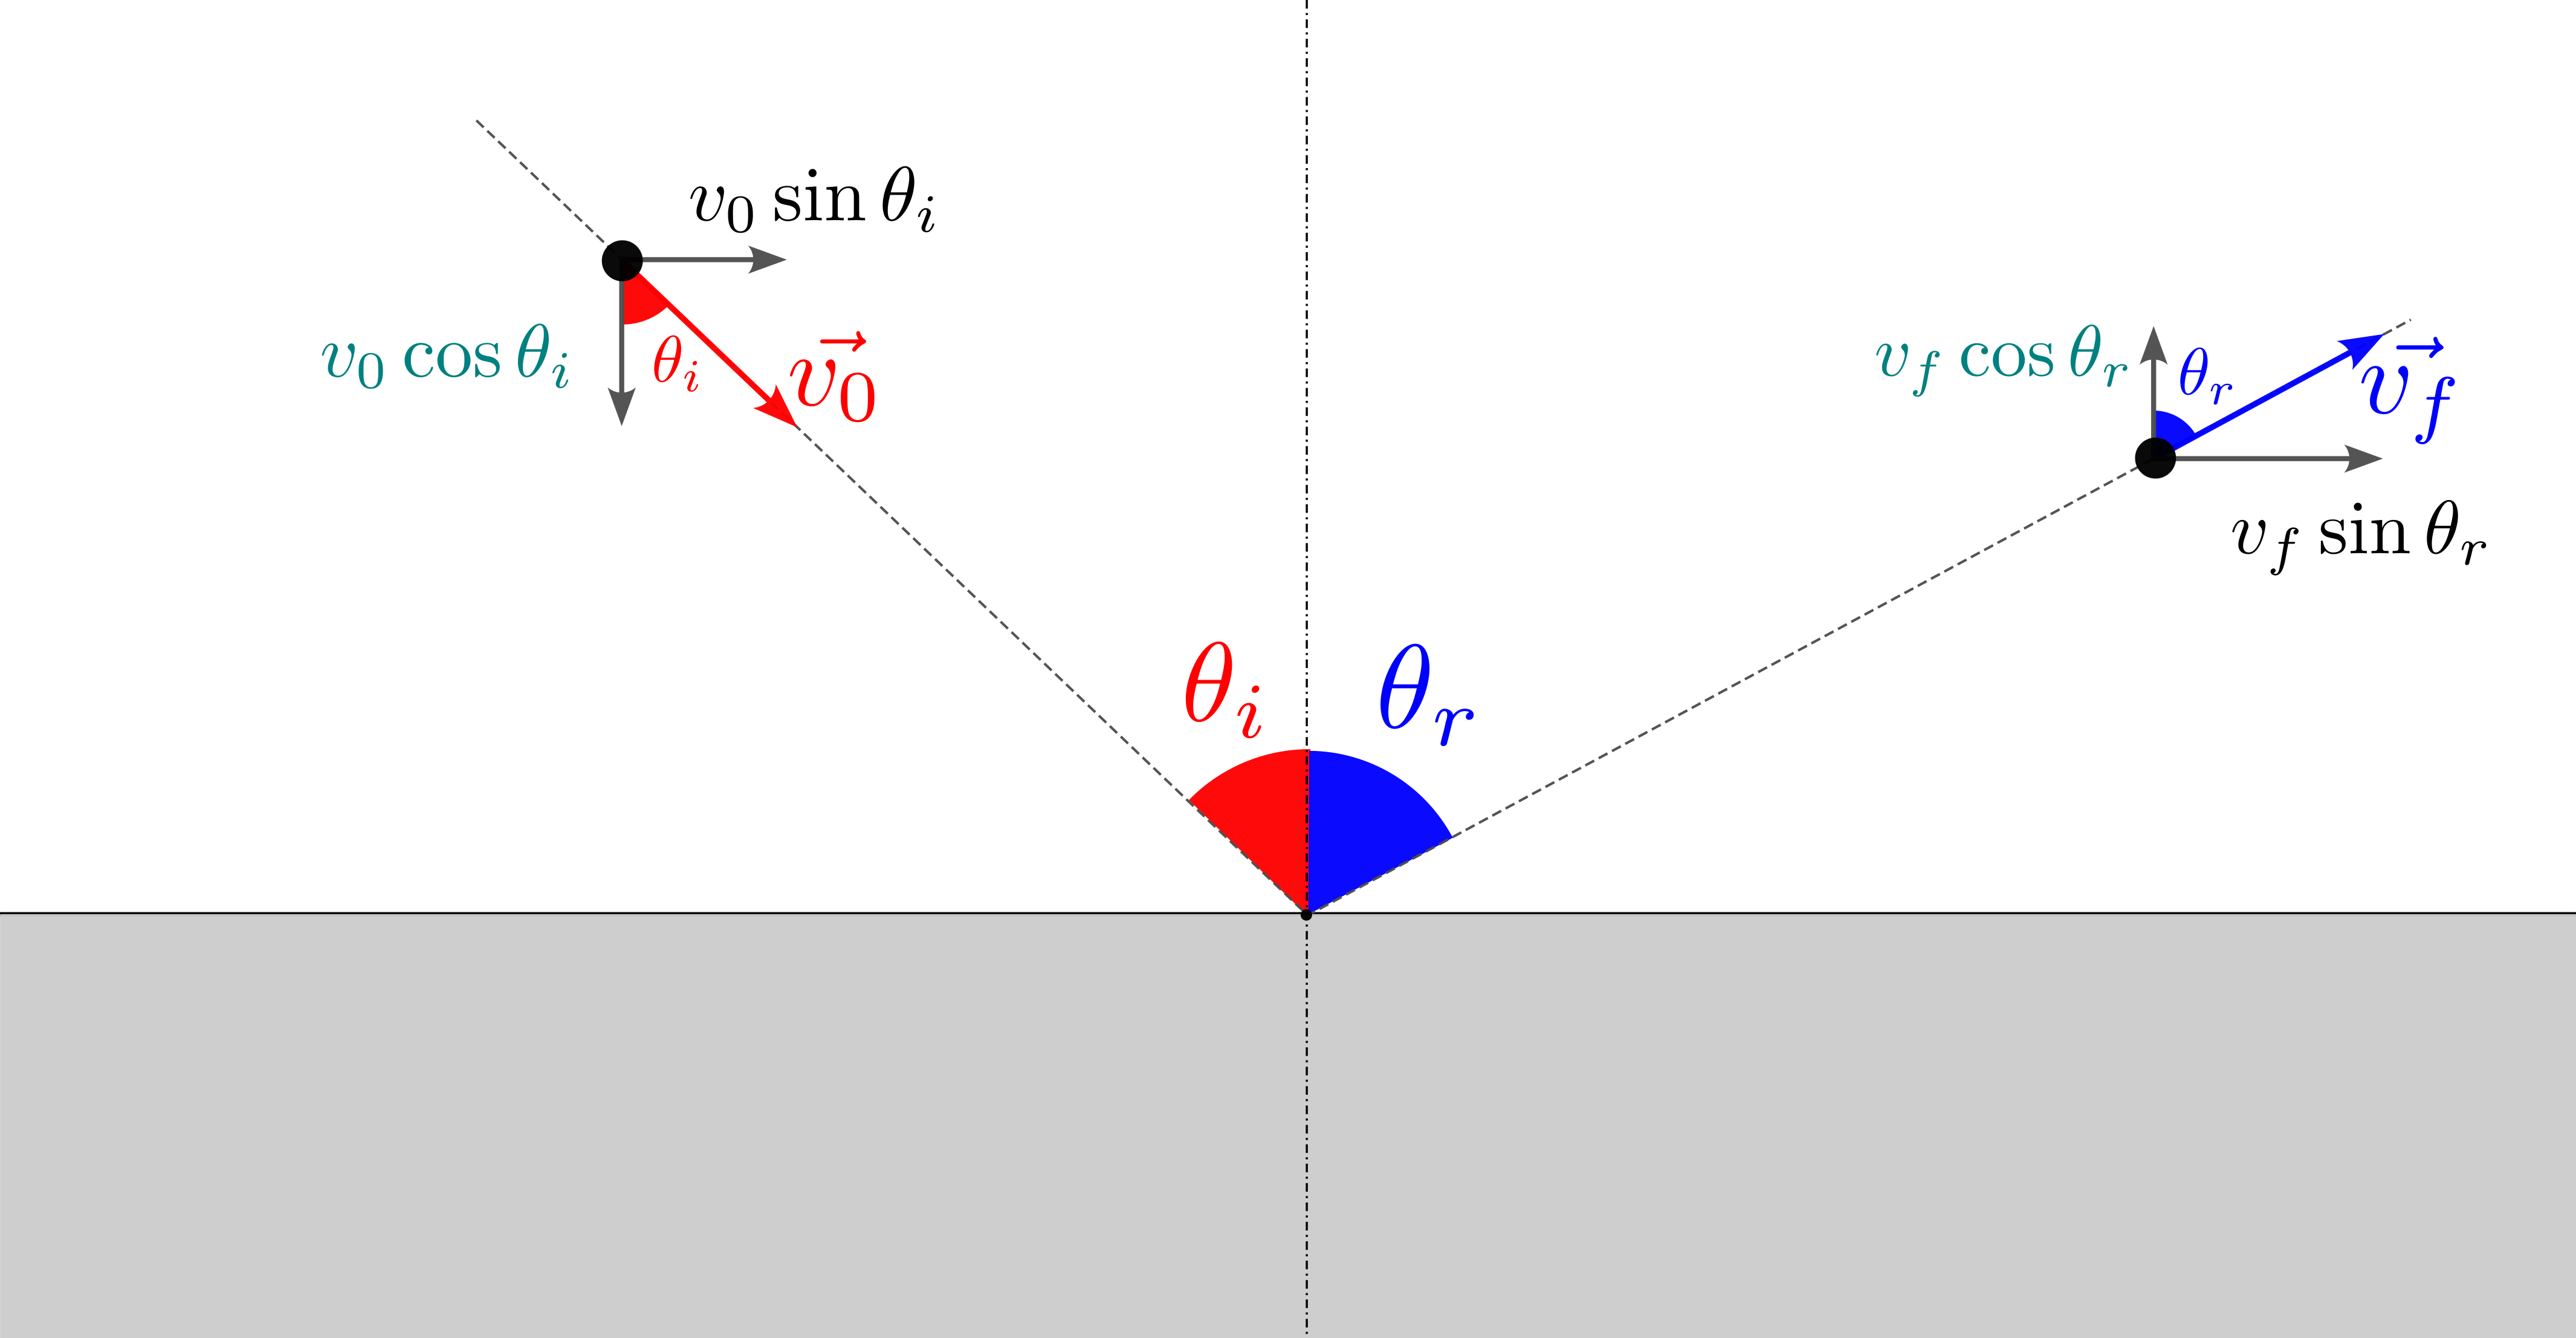
\includegraphics[width=.8\textwidth]{img/reflexao-newton.png}
            \caption{Reflexão corpuscular da luz.}
            \label{fig:reflexao-newton}
        \end{figure}
        \vspace*{20pt}
        
        Supondo que a colisão entre a partícula de luz e a interface seja puramente inelástica, a força resultante que a partícula faz sobre a superfície é normal $\vec{F}_{p,s}$, e pela terceira Lei de Newton a força que a superfície faz sobre a partícula é $-\vec{F}_{s,p}$. Em virtude disto, esta força é responsável por alterar somente a componente vertical da velocidade, mantendo a componente horizontal intacta. O momento linear e a energia são conservados, de maneira que podemos escrever as relações

        \begin{subequations}
            \begin{align}
                \vec{p}_0&=\vec{p}_f\\
                E_0&=E_f
            \end{align}
        \end{subequations}

        \begin{subequations}
            \begin{align}
                mv_0\sin\theta_i&=mv_f\sin\theta_r\label{eq:cons-momento-pla3}\\
                \frac{1}{2}mv_0^2&=\frac{1}{2}mv_f^2\label{eq:cons-energia-pla3}
            \end{align}
        \end{subequations}

        Não havendo dissipação da energia (colisão inelástica) a velocidade final da partícula de luz deve ser igual, em módulo, a velocidade inicial de modo que
        \begin{align}
            \begin{split}
                \sin\theta_i&=\sin\theta_r\\
                \theta_i&=\theta_r
            \end{split}
        \end{align}
    \end{proof}
    Fica assim demostrada a reflexão da luz na teoria corpuscular de Newton

    \vspace{50pt}
    \noindent \emph{3º Momento:} Refração corpuscular
	\par\noindent\rule{.3\textwidth}{.5pt}    
    \par\noindent \textbf{Tempo previsto: }15 minutos

    \noindent \textbf{Dinâmica:} Relembrar o fenômeno da refração observado na simulação, e pegar como exemplo a luz vindo do ar para a água. Os alunos devem lembrar que neste caso, a luz refratada sofre um desvio se aproximando-se da normal à superfície no ponto de contato.

    Vamos agora analisar este fenômeno dentro do ponto de vista da teoria corpuscular newtoniana.

    A exposição feita nesta parte deve seguir de forma semelhar a anterior, fazendo-se sempre argumentações e conduções sem exibir críticas ao modelo.

    \begin{proof}
        Seja uma partícula de luz viajando no ar com velocidade inicial $\vec{v}_0$. Se ao passar de um meio menos denso (ar) para um meio mais denso (água), observa-se uma mudança na trajetória da partícula, de modo tal que sua trajetória no meio mais denso encontra-se mais próximo à normal. Deve atuar, no instante entre a passagem entre os meios, uma força $\vec{F}$ responsável por alterar a componente vertical da partícula nesta direção, a \autoref{fig:refracao-newton} sintetiza a situação antes e depois da partícula de luz entrar na água
        
    \vspace*{20pt}
    \begin{figure}[!ht]
        \centering
        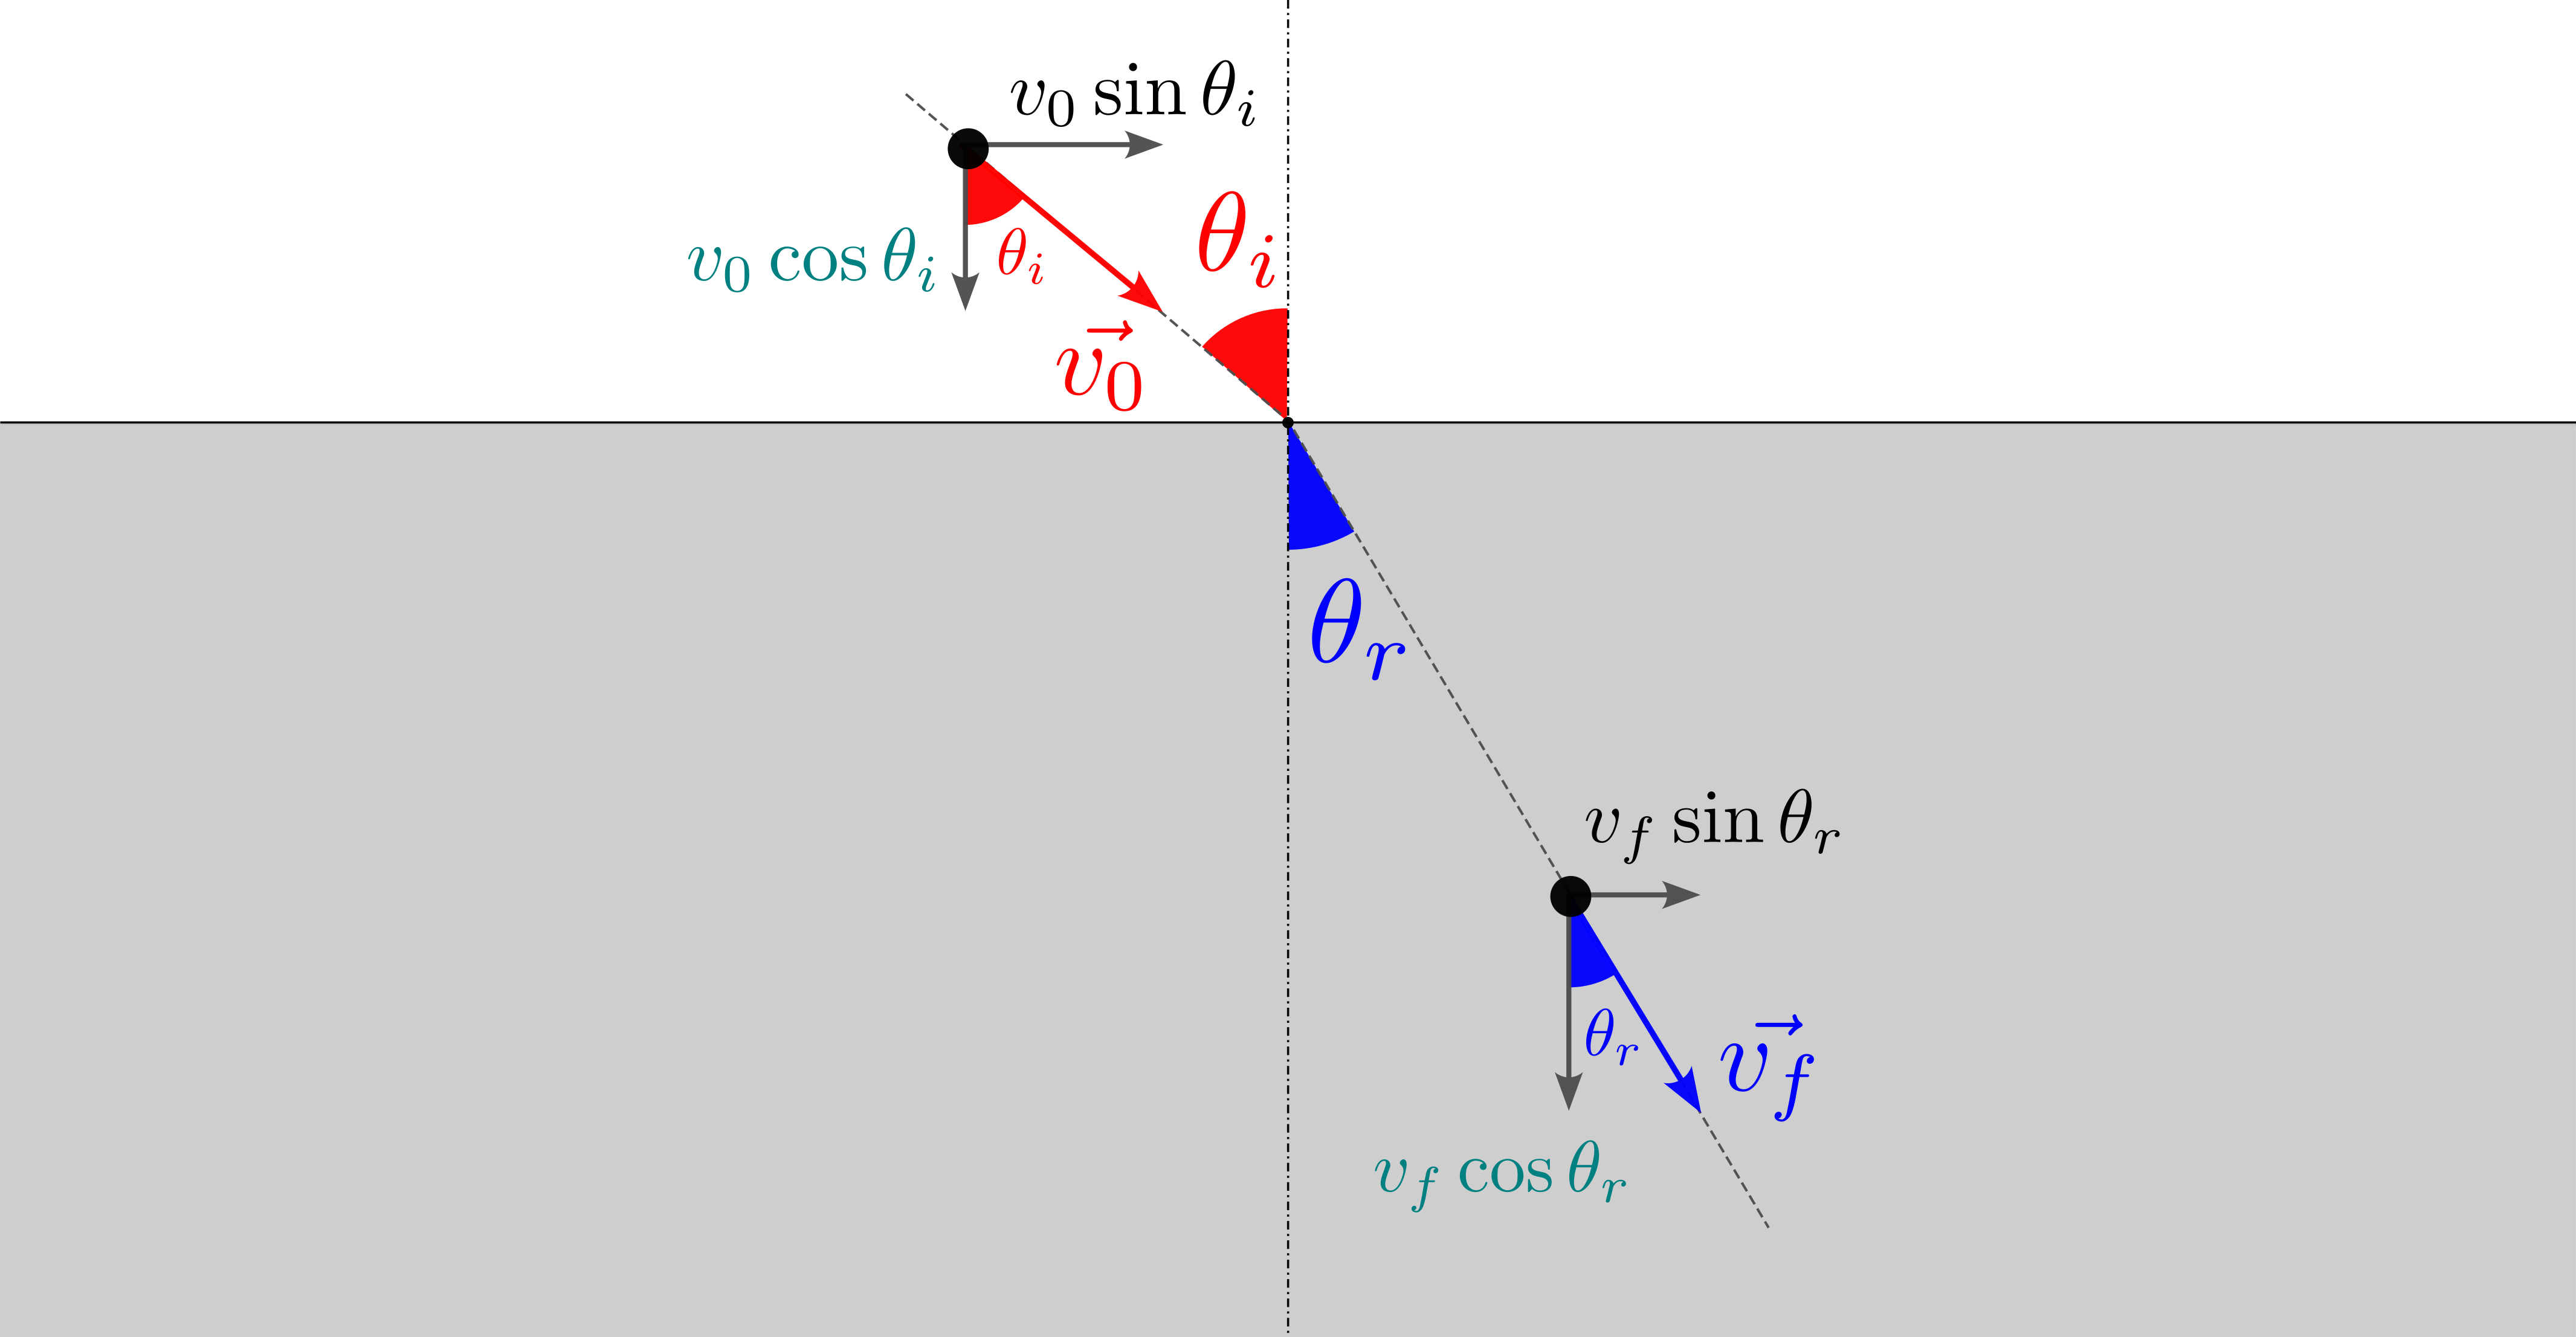
\includegraphics[width=0.8\textwidth]{img/refracao-newton.png}
        \caption{Refração corpuscular da luz.}
        \label{fig:refracao-newton}
    \end{figure}
    \vspace*{20pt}

    A componente horizontal não se altera, de modo que

    \begin{align}
        \begin{split}
            \frac{\sin\theta_i}{\sin\theta_r}&=\frac{v_f}{v_0}
        \end{split}
    \end{align}

    Sabendo que $\theta_i>\theta_r$, decorre que
    \begin{align}
        \frac{\sin\theta_i}{\sin\theta_r}&>1
    \end{align}

    como consequência
    \begin{align}
        v_f&>v_0
    \end{align}

    Ou seja, a velocidade da luz na água deve ser maior do que no ar.
    \end{proof}

    
    \newpage
    %-----------------------------------------------%
% Início do plano de aula
%-----------------------------------------------%
\thispagestyle{empty}
\begin{center}
	\begin{minipage}[!]{\linewidth}
        \begin{minipage}[!]{.19\linewidth}
            
\includegraphics[width=\linewidth]{img/logo.png}           
        \end{minipage}
        \begin{minipage}[!]{.8\linewidth}
            \center
            \ABNTEXchapterfont\normalsize\MakeUppercase{\imprimirinstituicao}
            \par
            \vspace*{10pt}                     
            \ABNTEXchapterfont\normalsize\MakeUppercase{\centro}
            \par
            \vspace*{10pt}           
            \ABNTEXchapterfont\normalsize\MakeUppercase{\disciplina}
        \end{minipage}        
    \end{minipage}
    \\ \vspace{0.5cm}
    \rule{\textwidth}{.5pt}   
\end{center}
    \textual
    \begin{center}
      \section{Ondas I}
      \par
    \end{center}
    
    \noindent \textbf{Estagiário(a): }\imprimirautor 
    
    \noindent \textbf{U.E.:} EEB Giovani Pasqualini Faraco
    
    \noindent \textbf{Série:} 2º Ano\hfill{}\textbf{Turma:} 2º--5
    
    \noindent \textbf{Aula:} 004\hfill{}\textbf{Data:} 21/10/2022\hfill{}\textbf{Duração:} $45\min$
    \rule{\textwidth}{.5pt}
    \bigskip{}  
    

    \noindent
    \begin{center}
      \textbf{Ondas: Grandezas Descritivas}
    \par\end{center}
    \vspace{20pt}
    \par\noindent\textbf{Resumo da aula:} Será introduzido o conceito de ondas de forma a dar suporte ao estudo da propagação luminosa, nesse formalismo.
    \vspace{20pt}
    \par\noindent \textbf{Habilidades BNCC:} EF09CI06; EF09CI04.    
    \vfill     
    \subsection*{Objetivo de Aprendizagem}
    \begin{itemize}
        \item Conhecer as principais grandezas do movimento oscilatório;
        \item Calcular a velocidade de uma onda qualquer com base em suas grandezas constituintes.
    \end{itemize}
    \medskip{}
    \vfill  
    \noindent \textbf{Núcleo Conceitual:} \emph{Ondulatória; comprimento de onda; período e frequência.}

    \newpage
    \section*{Procedimento Didático} 
    \noindent \emph{1º Momento:} Introdução ao modelo ondulatório
    \par\noindent\rule{.3\textwidth}{.5pt}  
    \par\noindent \textbf{Tempo previsto:} 10 minutos

    \noindent \textbf{Dinâmica:} Na aula passada vimos como descrever os fenômenos de reflexão e a refração da luz usando o modelo corpuscular construído por Newton.

    Conduzir a turma para a  síntese obtida na aula passada, em que: o ângulo de incidência e o ângulo refletido são sempre iguais, concordando com o que observa-se para o fenômeno, e para a refração, o modelo corpuscular, prevê uma velocidade maior da luz em meios mais densos como a água, do que em meios menos densos como o ar.

    Citar que a teoria newtoniana não era a única que buscava uma melhor compreensão para os fenômenos luminosos, havia naquela época, uma teoria concorrente baseada em observações que também se propunha a explicar estes fenômenos, mas de maneira diferente, a teoria ondulatória da luz, defendida principalmente por Christiaan Huygens (1629– 1695). 

    Para compreender melhor este modelo, precisaremos conhecer algumas grandezas relacionadas ao movimento oscilatório.

    \vspace*{20pt}
    \noindent \emph{2º Momento:} Grandezas fundamentais do movimento oscilatório
    \par\noindent\rule{.3\textwidth}{.5pt}  
    \par\noindent \textbf{Tempo previsto:} 20 minutos

    \noindent \textbf{Dinâmica:} Esquematizar no quadro o desenho de uma onda propagando-se em uma corda, e definir o comprimento de onda $\lambda$ como a distância entre dois picos ou dois vales consecutivos. O quadro deve ficar mais ou menos similar a \autoref{fig:comprimento-de-onda} a seguir:
    \vspace*{20pt}
    \begin{figure}[!ht]
        \centering
        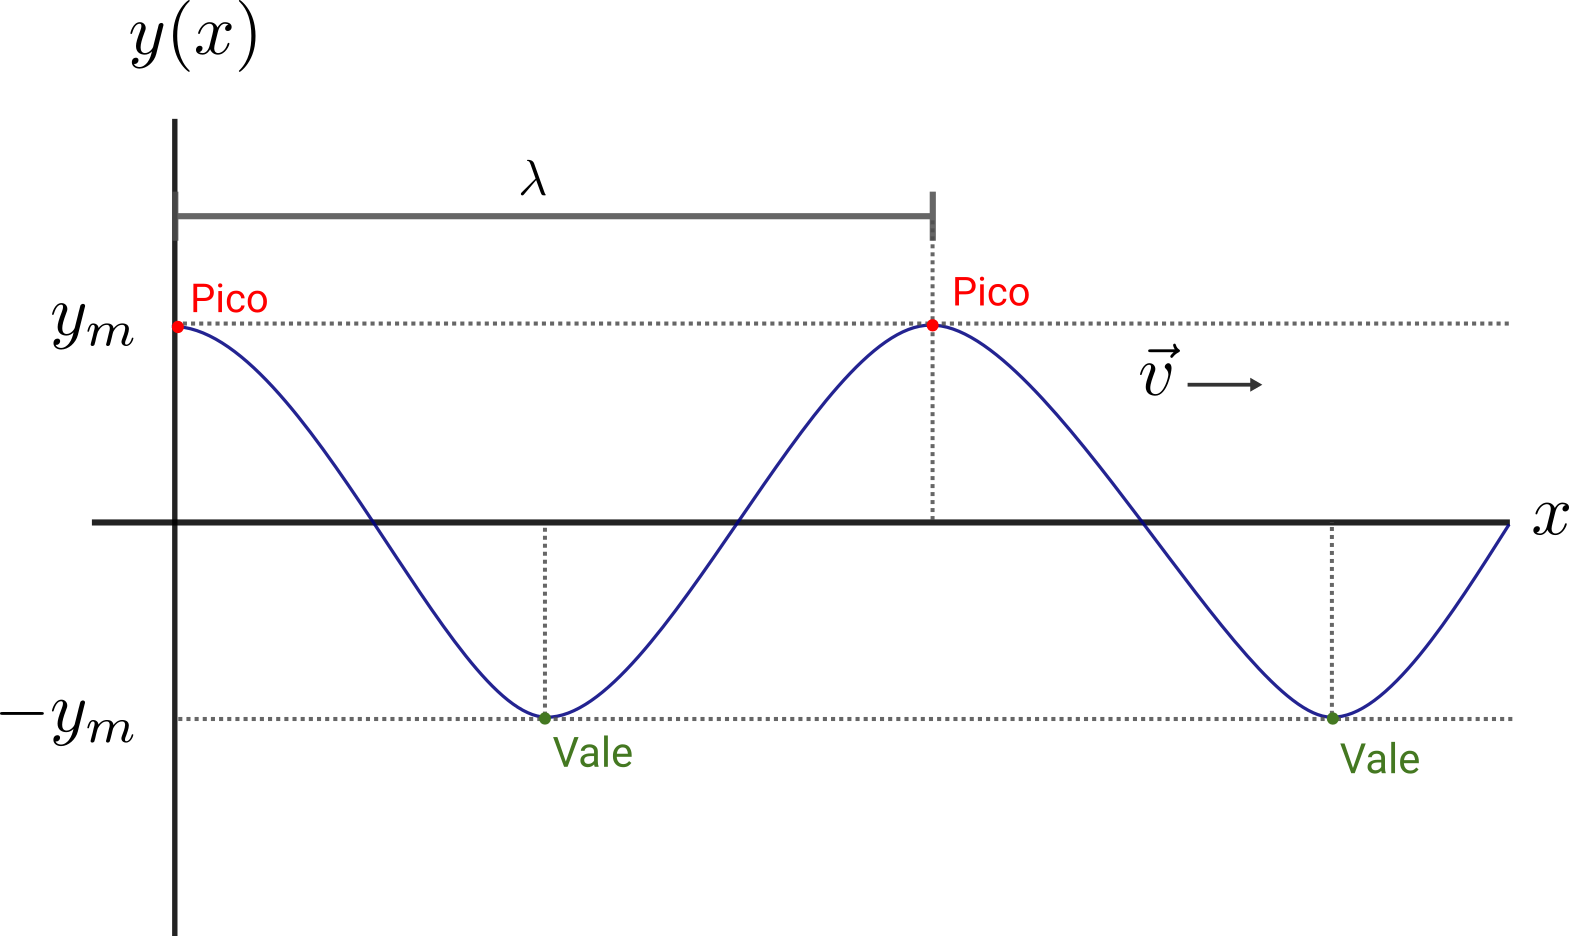
\includegraphics[width=0.6\textwidth]{img/lambda-1.png}
        \caption{Comprimento de onda $\lambda$ em uma corda}
        \label{fig:comprimento-de-onda}
    \end{figure}
    \vspace*{20pt}

    De forma similar, definir o período de uma onda em uma corda, como o intervalo de tempo necessário para que a onda complete um ciclo de oscilação. A medir que for introduzindo os conceitos, desenhar no quadro uma figura semelhante a \autoref{fig:periodo-de-onda} para auxiliar a compreensão dos estudantes.

    \vspace*{20pt}
    \begin{figure}[!ht]
        \centering
        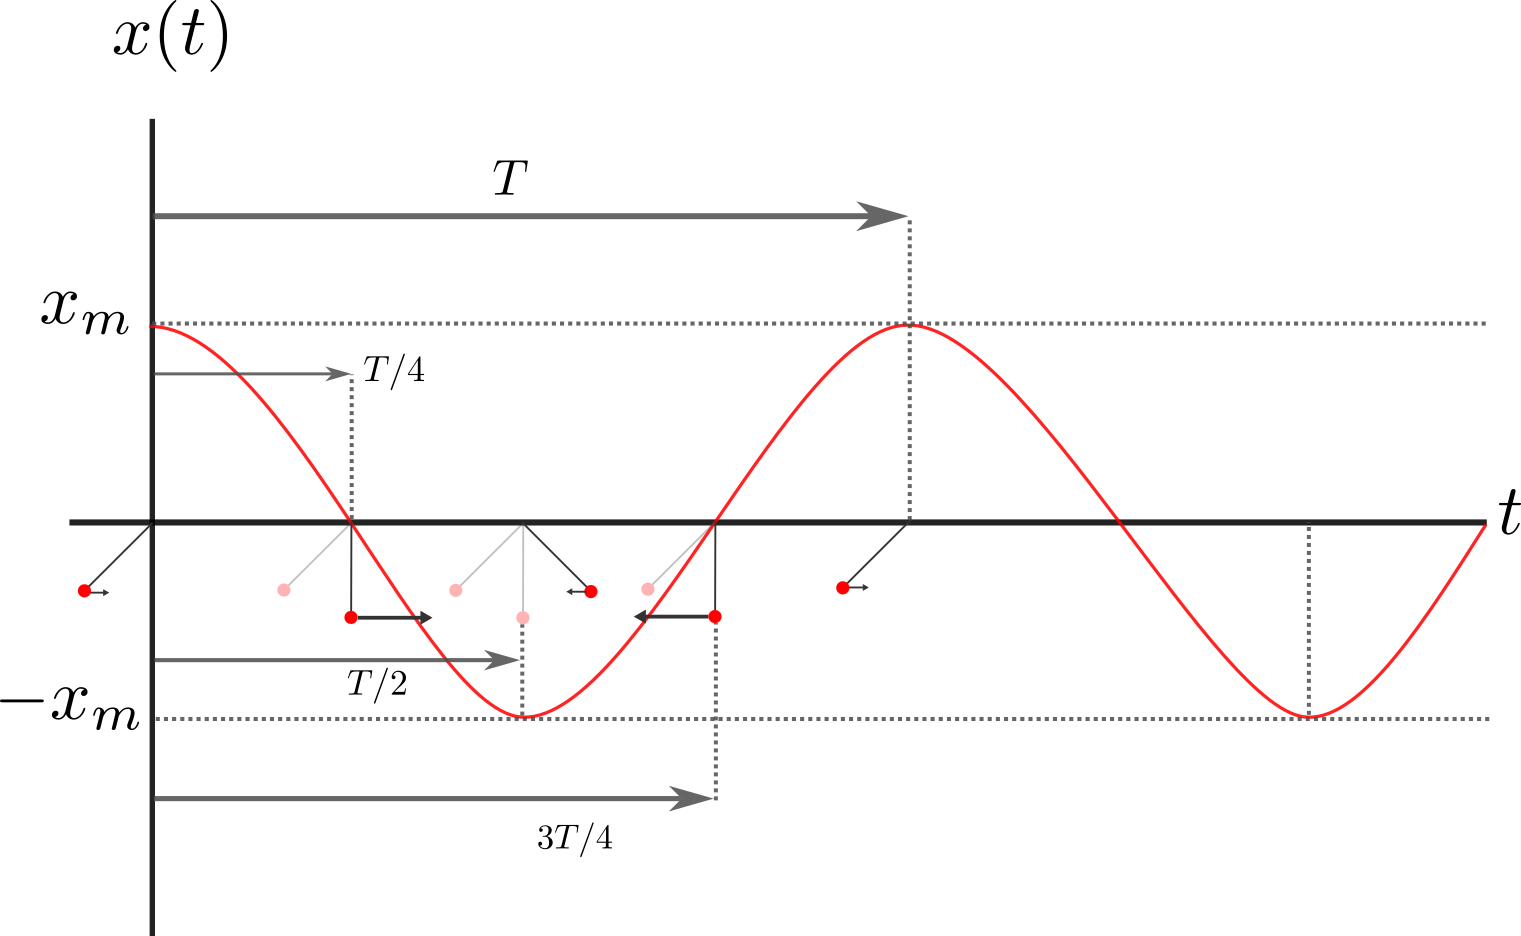
\includegraphics[width=0.6\textwidth]{img/periodo-1.png}
        \caption{Período $T$}
        \label{fig:periodo-de-onda}
    \end{figure}
    \vspace*{20pt}

    Definir a frequência como a quantidade de ciclos que a onda completa em um intervalo de tempo determinado.
    \begin{align}
        f&=\frac{1}{T}
    \end{align}

    \vspace*{20pt}
    \noindent \emph{3º Momento:} Velocidade de uma onda
    \par\noindent\rule{.3\textwidth}{.5pt}  
    \par\noindent \textbf{Tempo previsto:} 15 minutos

    \noindent \textbf{Dinâmica:} A velocidade de propagação de uma onda pode ser calculada usando o conceito de velocidade escalar média visto no primeiro ano.

    \begin{align}
        v&=\frac{\Delta S}{\Delta t}
    \end{align}

    Esta relação para uma onda fica

    \begin{align}
        v&=\frac{\lambda}{T}
    \end{align}
    o que também pode ser escrito em termos da frequência como
    \begin{align}
        v&=\lambda f
    \end{align}

    Após estabelecida a equação da velocidade de uma onda, pedir que diferentes grupos de alunos estimem a velocidade das ondas do espectro visível a partir dos dados da \autoref{tab:alguns-espectros-do-visivel}:
    \vspace*{1pt}
    
    \begin{table}[!ht]
        \centering
        \begin{tabular}{|c|c|c|}
        \hline
        \textbf{Cor}      & \textbf{$\lambda(\textrm{nm})$} & \textbf{Frequência $f(10^{12}\textrm{Hz})$} \\ \hline
        \textbf{Vermelho} & 625                             & 480                                         \\ \hline
        \textbf{Laranja}  & 590                             & 510                                         \\ \hline
        \textbf{Amarelo}  & 565                             & 530                                         \\ \hline
        \textbf{Verde}    & 500                             & 600                                         \\ \hline
        \end{tabular}
        \caption{Comprimentos de onda $\lambda$ e frequências $f$ de algumas faixas de valores do espectro visível.}
        \label{tab:alguns-espectros-do-visivel}
    \end{table}
    \vspace*{10pt}

    \noindent Todos devem encontrar valores muito próximos a $2,99\times 10^8\mps$. Questionar o motivo pelo qual todos encontraram valores muito próximos, e se já conhecem este valor de velocidade. Relacionar esta velocidade com a velocidade da luz no vácuo e justificar que pelo fato do ar, ser o meio material cujo o qual oferece a menor resistência à passagem da luz, os físicos normalmente utilizam a velocidade da luz no ar igual à velocidade da luz no vácuo.
    
    Análogo ao que foi feito pra velocidade da luz, sugerir que a partir da \autoref{tab:notas-musicais} logo a abaixo estimem a velocidade do som
    \vspace*{10pt}
    
    \begin{table}[!ht]
        \centering
        \begin{tabular}{|c|c|c|}
        \hline
        \textbf{Nota} & \textbf{$\lambda(\textrm{m})$} & \textbf{Frequência $f(\textrm{Hz})$} \\ \hline
        \textbf{C}    & 21,04                          & 16,35                                \\ \hline
        \textbf{D}    & 18,74                          & 18,35                                \\ \hline
        \textbf{E}    & 16,70                          & 20,60                                \\ \hline
        \textbf{F}    & 15,76                          & 21,82                                \\ \hline
        \textbf{G}    & 14,04                          & 24,50                                \\ \hline
        \textbf{A}    & 12,51                          & 27,50                                \\ \hline
        \textbf{B}    & 11,14                          & 30,86                                \\ \hline
        \end{tabular}
        \caption{Comprimentos de onda $lambda$ e frequências $f$ de algumas notas musicais.}
        \label{tab:notas-musicais}
    \end{table}
    \vspace*{10pt}
    
    Dedicar o restante da aula para discussão destes resultados e tiragem de dúvidas sobre a exposição.

    
    \newpage
    %-----------------------------------------------%
% Início do plano de aula
%-----------------------------------------------%
\thispagestyle{empty}
\begin{center}
	\begin{minipage}[!]{\linewidth}
        \begin{minipage}[!]{.19\linewidth}
            
\includegraphics[width=\linewidth]{img/logo.png}           
        \end{minipage}
        \begin{minipage}[!]{.8\linewidth}
            \center
            \ABNTEXchapterfont\normalsize\MakeUppercase{\imprimirinstituicao}
            \par
            \vspace*{10pt}                     
            \ABNTEXchapterfont\normalsize\MakeUppercase{\centro}
            \par
            \vspace*{10pt}           
            \ABNTEXchapterfont\normalsize\MakeUppercase{\disciplina}
        \end{minipage}        
    \end{minipage}
    \\ \vspace{0.5cm}
    \rule{\textwidth}{.5pt}   
\end{center}
    \textual
    \begin{center}
      \section{Ondas II}
      \par
    \end{center}
    
    \noindent \textbf{Estagiário(a): }\imprimirautor 
    
    \noindent \textbf{U.E.: }EEB Giovani Pasqualini Faraco
    
    \noindent \textbf{Série: }2º Ano\hfill{}\textbf{Turma: }2º--5
    
    \noindent \textbf{Aula:} 005\hfill{}\textbf{Data:} 04/11/2022\hfill{}\textbf{Duração:} $45\min$
    \rule{\textwidth}{.5pt}
    \bigskip{}  
    

    \noindent
    \begin{center}
      \textbf{O princípio de Huygens}
    \par\end{center}
    \vspace{20pt}
    \noindent \textbf{Resumo da aula:} Com auxílio de simulações computacionais, apresentar o princípio de Huygens como base para a construção do modelo ondulatório para a Luz.
    \smallskip
    \par\noindent \textbf{Habilidades BNCC:} EM13CNT201.
    \medskip
    \subsection*{Objetivo de Aprendizagem}
    \begin{itemize}
        \item Conhecer o princípio de Hyugens e sua importância para a construção de um modelo ondulatório para a luz. 
    \end{itemize}    
    \bigskip{}    
    \noindent \textbf{Núcleo Conceitual:} \emph{Teoria ondulatória da luz; propagação.}
    \newpage
    

    \section*{Procedimento Didático} 
    \noindent\emph{1º Momento:} Problematização Inicial
    \par\noindent\rule{.3\textwidth}{.5pt}  
    \par\noindent\textbf{Tempo previsto:} 10 minutos
    \smallskip
    \par\noindent\textbf{Dinâmica:} Iniciar a aula recapitulando o modelo corpuscular de newton, focar a atenção para uma problemática em que Newton havia estudado, mas não conseguiu tecer alguma explicação utilizando o modelo corpuscular, o fenômeno é a difração.

    Mostrar algumas imagens da difração da Luz, como por exemplo a difração da luz por uma lâmina fina, questioná-los como seria possível, a luz contornar objetos na teoria corpuscular. Abrir a simulação do Phet e executar as simulações da imagem da \autoref{fig:difraction}, explicando detalhadamente o que está ocorrendo 

    \vspace*{10pt}
    \begin{figure}[!ht]        
        \centering              
        \subfloat[\label{fig:difraction-1}]{
            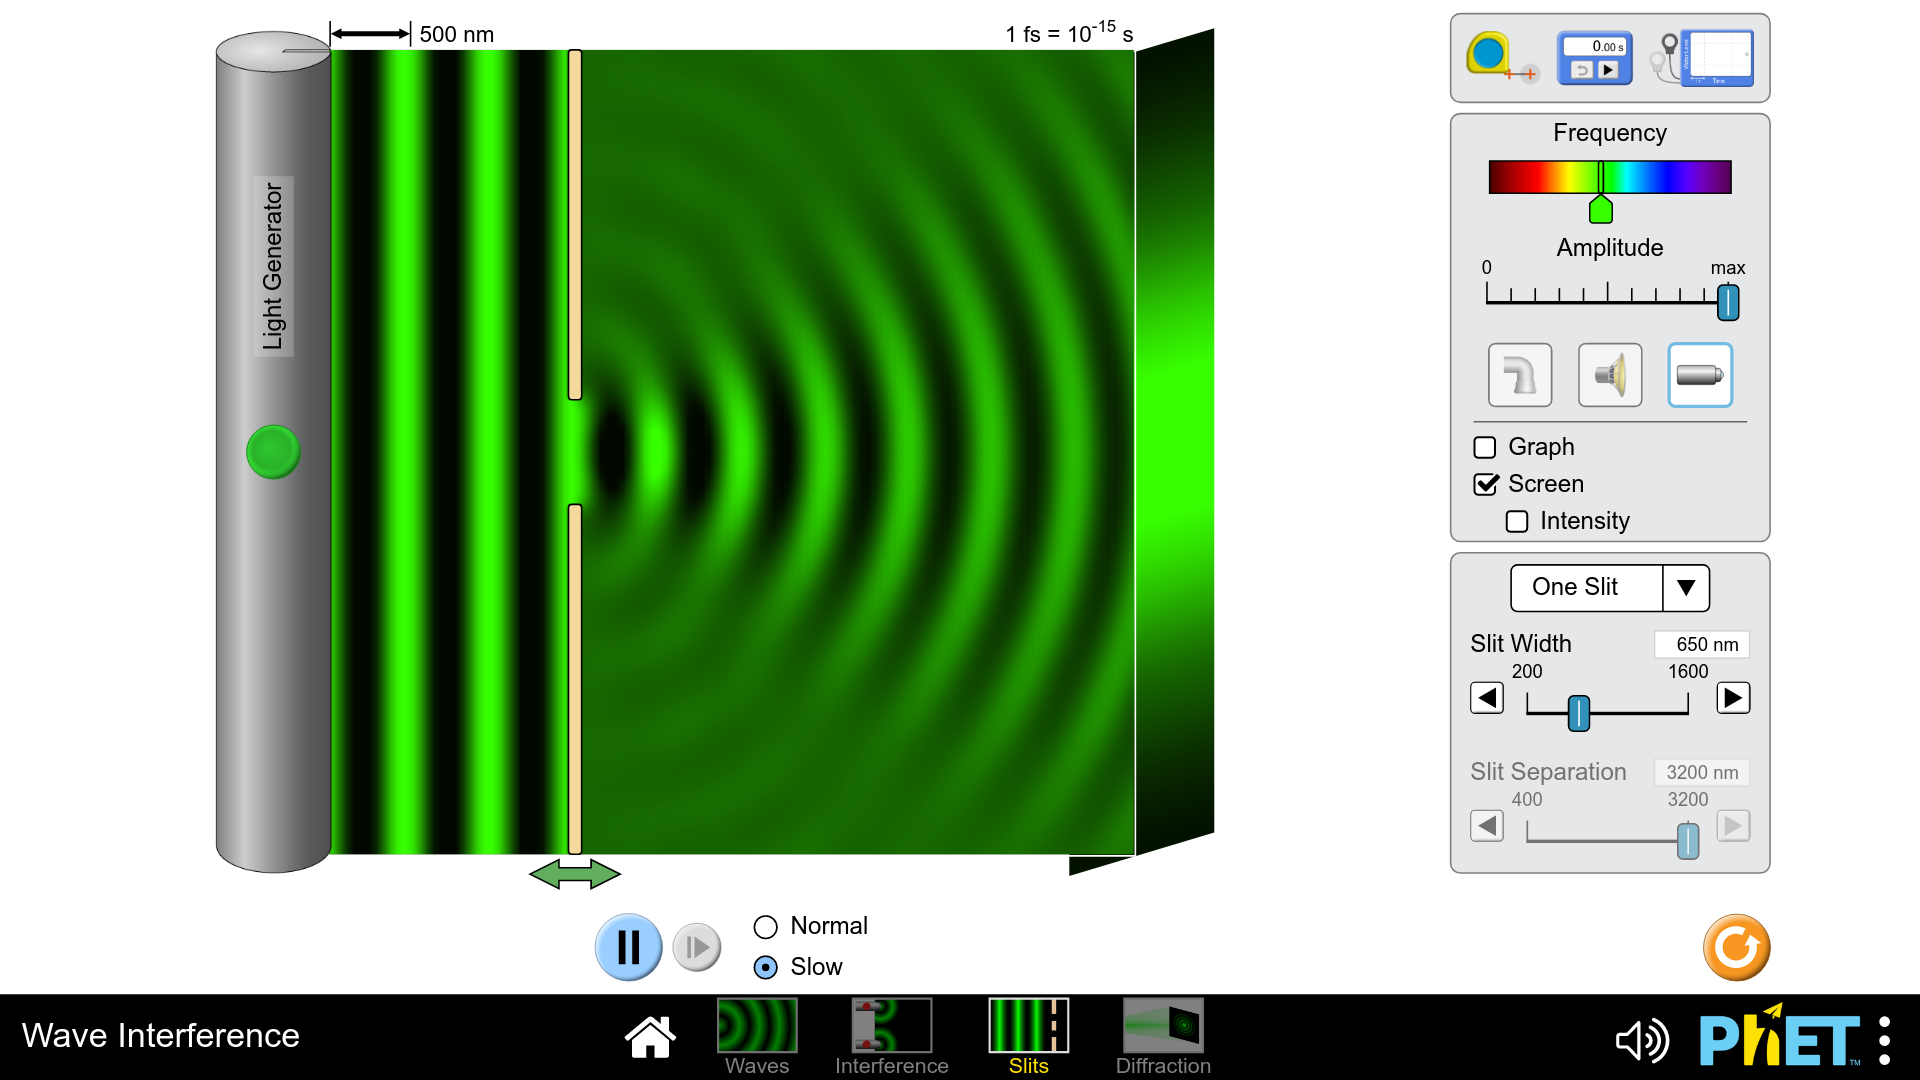
\includegraphics[width=.45\textwidth]{img/difraction-1.png}
        }\hfill
        \subfloat[\label{fig:difraction-2}]{
            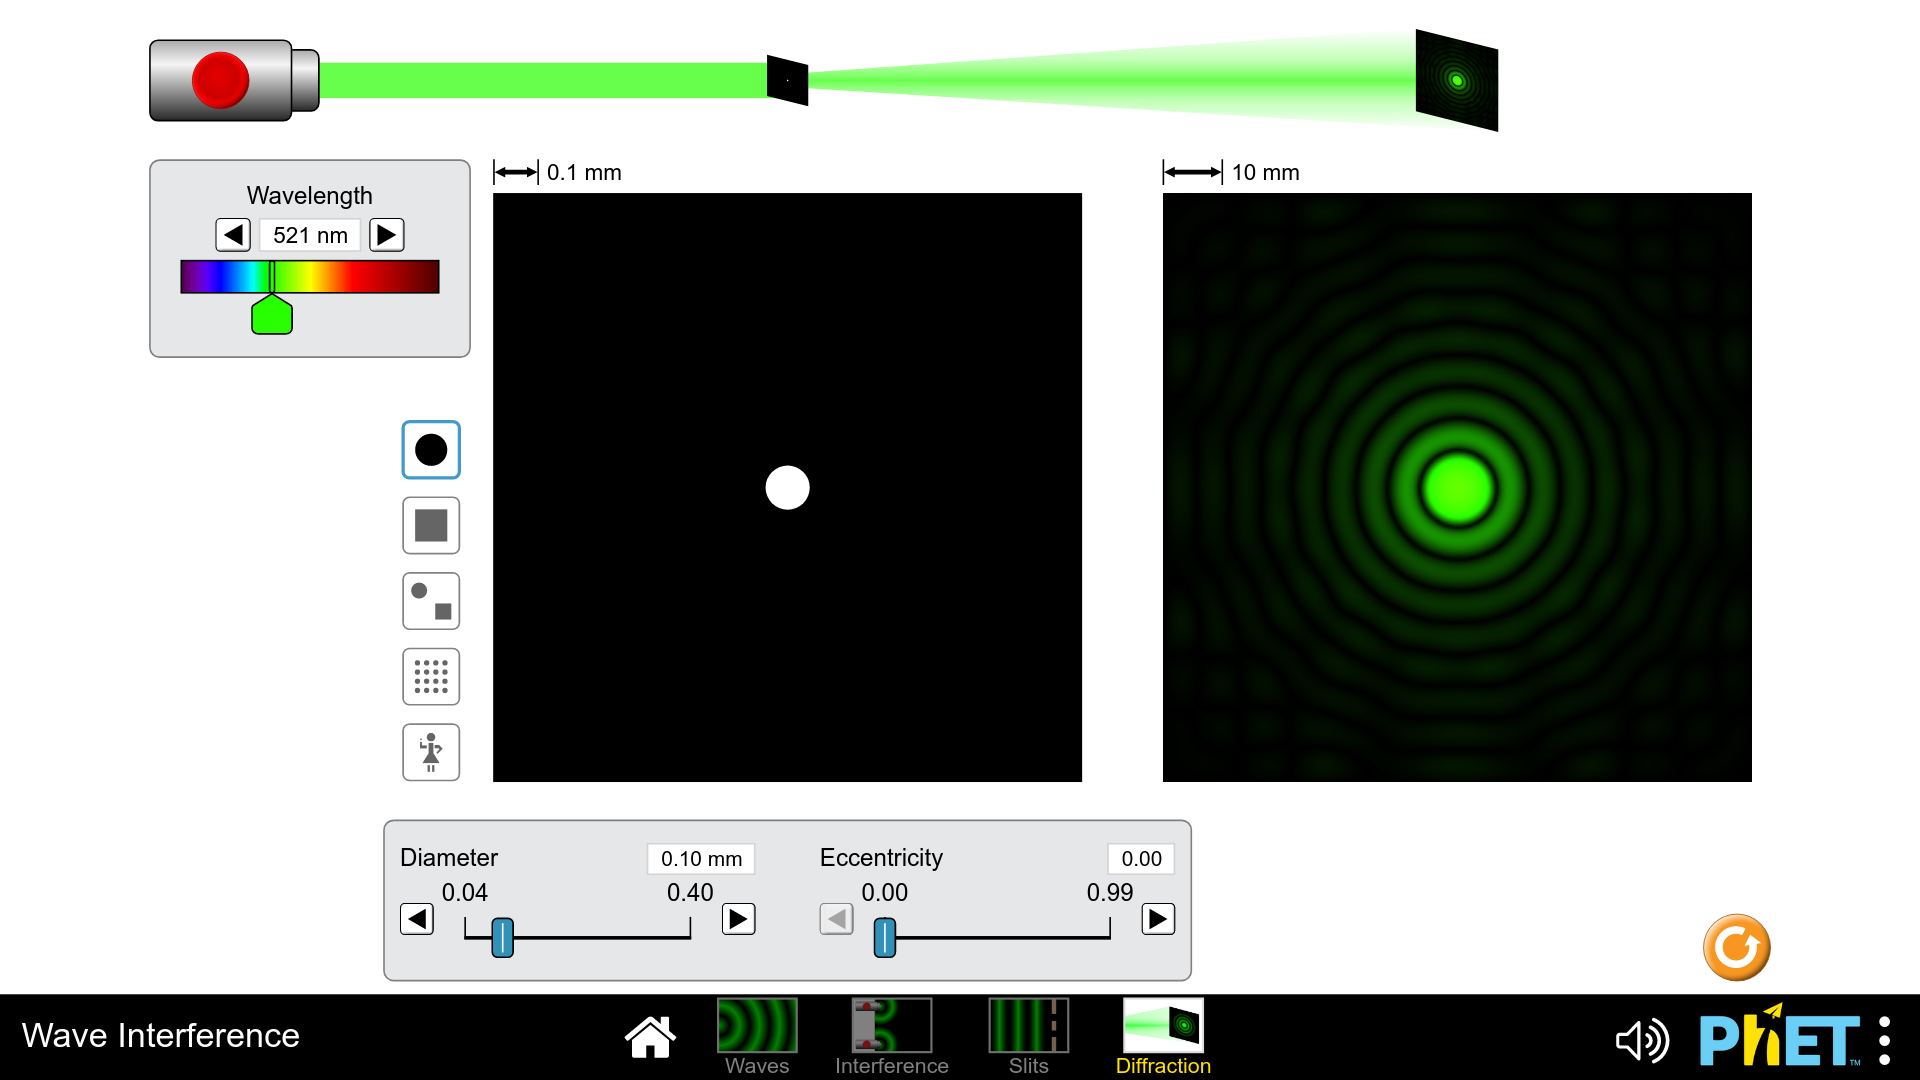
\includegraphics[width=.45\textwidth]{img/difraction-2.png}
        }        
        \caption{Simulação \emph{Phet} em (a), um feixe de ondas planas, passa por um orifício de uma determinada largura, o encurvamento das ondas é visto após o orifício. Em (b), tem-se as figuras de interferência formada num anteparo, ao fazer um feixe de luz atravessar um orifício circular.}
        \label{fig:difraction}
    \end{figure}
    \vspace*{10pt}

    Deixar claro que a simulação faz uso de instrumentos que não existiam à época de Newton e Huygens, mas estes cientistas, conheciam estes fenômenos, inclusive o próprio Newton já havia observado o mesmo fenômeno ocorrendo em lâminas delgadas. Este fenômeno fica bem compreendido por um artifício muito engenhoso estabelecido por Hyugens mo modelo ondulatório, que é o \emph{Princípio de Huygens}
    

% Segundo os autores é nessa etapa que se apresentam questões e/ou situações para discussão com os alunos, visando relacionar o estudo de um conteúdo com situações reais que eles conhecem e presenciam, mas que não conseguem interpretar completa ou corretamente porque provavelmente não dispõem de conhecimentos científicos suficientes. Ou seja, é na problematização que se deseja aguçar explicações contraditórias e localizar as possíveis limitações do conhecimento que vem sendo expressado, quando este é cotejado com o conhecimento científico que já foi selecionado para ser abordado (Delizoicov, Angotti e Pernambuco, 2002, p. 201). Portanto, esse primeiro momento é caracterizado pela compreensão e apreensão da posição dos alunos frente ao tema. É desejável ainda, que a postura do professor se volte mais para questionar e lançar dúvidas sobre o assunto que para responder e fornecer explicações.
    \newpage
    \bigskip{}
    \noindent\emph{2º Momento:} Organização do Conhecimento
    \par\noindent\rule{.3\textwidth}{.5pt}  
    \par\noindent\textbf{Tempo previsto:} 10 minutos
    \smallskip
    \par\noindent\textbf{Dinâmica:} Abrir a \href{https://simphy.com/other-apps/huygen-principle/}{simulação} e iniciar a explicação partindo do caso simples: um ponto gerando uma frente de onda, tal como a \autoref{fig:huygens-1-2}

    \vspace*{10pt}
    \begin{figure}[!ht]        
        \centering              
        \subfloat[\label{fig:huygens-1}]{
            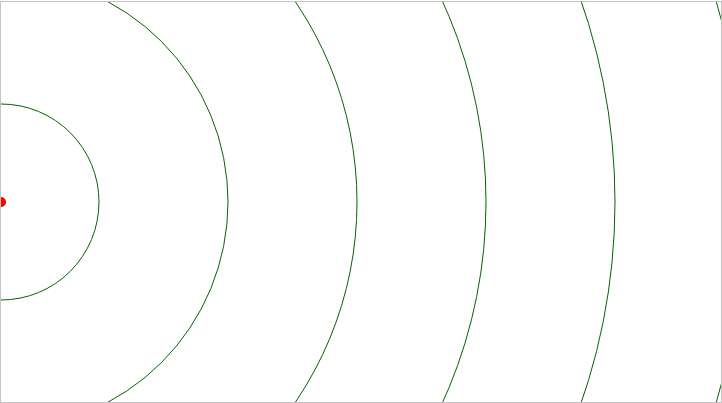
\includegraphics[width=.45\textwidth]{img/principio-huygens-ponto.png}
        }\hfill
        \subfloat[\label{fig:huygens-2}]{
            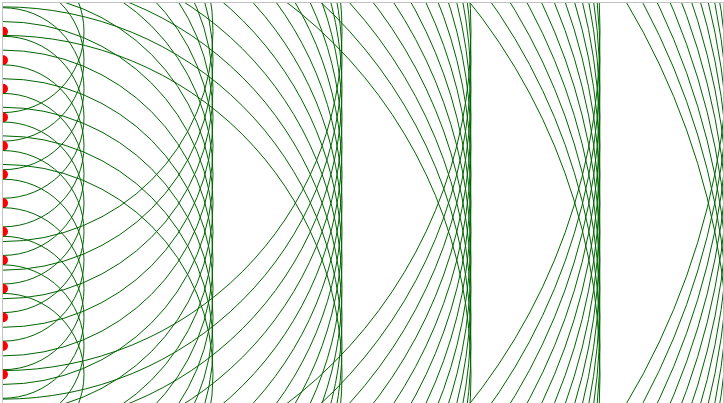
\includegraphics[width=.45\textwidth]{img/principio-huygens-onda-plana.png}
        }        
        \caption{Simulação \emph{Princípio de Huygens} em (a), um ponto simulando um orifício gerador de frentes das frentes de onda. Em (b), vários pontos simulando frentes de ondas planas.}
        \label{fig:huygens-1-2}
    \end{figure}
    \vspace*{10pt}

    Enunciar o princío de Huygens da seguinte maneira:

    \begin{principio}[Huygens]
        Cada ponto de uma frente de onda comporta-se como uma fonte geradora de ondas, que são produzidas com as mesmas características da original.
    \end{principio}

    Por características originais, Huygens quer dizer, mesmo comprimento de onda e mesma frequência.

    Vamos utilizar este princípio para compreender a propagação da luz de passando de um meio para o outro e ver como os fenômenos da reflexão e refração são entendidos no modelo ondulatório.
    

 
    % \begin{figure}[!ht]
    %     \centering
    %     \begin{tikzpicture}[scale=0.8]
        
    %         % define coordinates
    %         \coordinate (O) at (0,0) ;
    %         \coordinate (A) at (0,4) ;
    %         \coordinate (B) at (0,-4) ;
            
    %         % media
    %         \fill[blue!25!,opacity=.3] (-4,0) rectangle (4,4);
    %         \fill[blue!60!,opacity=.3] (-4,0) rectangle (4,-4);
    %         \node[right] at (2,2) {Ar};
    %         \node[left] at (-2,-2) {Água};
        
    %         % axis
    %         \draw[dash pattern=on5pt off3pt] (A) -- (B) ;
        
    %         % rays
    %         \draw[red,ultra thick,reverse directed] (O) -- (130:5.2);
    %         \draw[blue,directed,ultra thick] (O) -- (-70:4.24);
    %         \draw[green,ultra thick,directed] (O) -- (50:5.2);
        
    %         % angles
    %         \draw (0,1) arc (90:130:1);
    %         \draw (0,-1.4) arc (270:290:1.4);
    %         \draw (0,1) arc (90:50:1);
    %         \node[] at (280:1.8)  {$\theta_{2}$};
    %         \node[] at (110:1.4)  {$\theta_{1}$};
    %         \node[] at (70:1.4)   {$\theta_{3}$};
    %     \end{tikzpicture}
    %     \caption{Caption}
    %     \label{fig:my_label}
    % \end{figure}

    % http://hyperphysics.phy-astr.gsu.edu/hbase/phyopt/huygen.html
    % https://simphy.com/other-apps/huygen-principle/
    % https://www.walter-fendt.de/html5/phen/refractionhuygens_en.htm
    

% Delizoicov e Angotti (1990, p. 29) explicam que nesse segundo momento os conhecimentos de Física necessários para a compreensão do tema e da problematização inicial devem ser sistematicamente estudados sob orientação do professor. Definições, conceitos, relações, leis, apresentadas no texto introdutório, serão agora aprofundados. De acordo com Albuquerque, Santos e Ferreira (2015, p. 467) esse é o momento em que os conhecimentos científicos passam a ser incorporados nas discussões. Os alunos começam a desenvolver uma compreensão a respeito da problematização ou situação inicial. Entretanto, para que isso ocorra, materiais devem ser consultados e atividades devem ser sugeridas para complementar as discussões, no sentido de incentivar e melhorar a sistematização dos conhecimentos. Nessa perspectiva, Delizoicov e Angotti (1990) vêm ressaltar a importância de diversificadas atividades, com as quais se poderá trabalhar para organizar a aprendizagem. Sugerem exposições, pelo professor, de definições e propriedades, além de formulações de questões (exercícios de fixação como dos livros didáticos), textos e experiências. Neste sentido, atualmente poderíamos acrescentar as mídias tecnológicas, como televisão, vídeos, filmes, programas tecnológicos, aplicativos de celulares, simulações, entre outros, de modo a auxiliar no processo da sistematização do conhecimento.

    \newpage
    \bigskip
    \noindent\emph{3º Momento:} Aplicação do Conhecimento
    \par\noindent\rule{.3\textwidth}{.5pt}  
    \par\noindent\textbf{Tempo previsto:} 10 minutos
    \smallskip
    \par\noindent\textbf{Dinâmica:} Abrir a próxima \href{https://www.walter-fendt.de/html5/phen/refractionhuygens_en.htm}{simulação}, passar as etapas desta última simulação de forma dialogada. A \autoref{fig:huygens-refracao-reflexao} a seguir mostra as duas situações que devem ser discutidas, para a refração e reflexão.

    
    \vspace*{10pt}
    \begin{figure}[!ht]        
        \centering              
        \subfloat[\label{fig:refracao-ondas}]{
            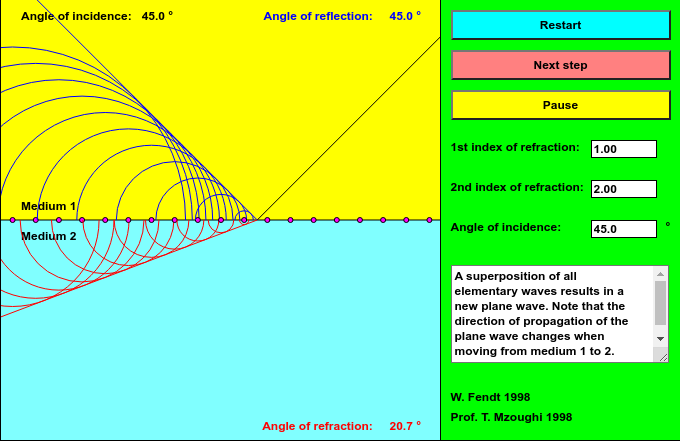
\includegraphics[width=.45\textwidth]{img/refracao-ondas-1.png}
        }\hfill
        \subfloat[\label{fig:reflexao-ondas}]{
            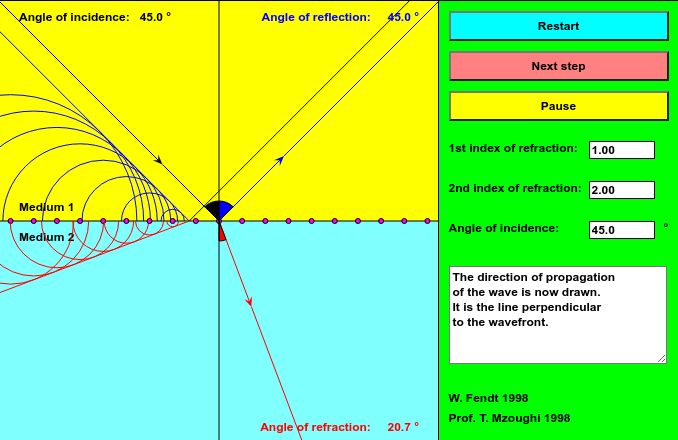
\includegraphics[width=.45\textwidth]{img/reflexao-ondas-1.png}
        }        
        \caption{Simulação \emph{Princípio de Huygens} em (a), uma frente de onda propagando-se do meio menos denso, com ângulo de 45\degree, para um mais denso, alterando a direção de propagação para 20,7\degree. As frentes de onda formadas após a interação com o meio, seguem o princípio de Huygens. Em (b) tem-se destacado as frentes de onda, deslocando-se perpendicularmente com relação a direção de propagação.}
        \label{fig:huygens-refracao-reflexao}
    \end{figure}
    \vspace*{10pt}

    Variar os parâmetros da simulação de forma a deixar claro a incidência perpendicular da frente de onda com relação à velocidade de propagação da mesma. Este fato vai ser importante para deduzir a lei de Snell na próxima aula.

    Por fim, chamar a atenção para a frente de onda refletida pelos pontos sobre a interface, se necessário pausar a simulação no exato momento em que a frente de onda refletida se encontra com o raio refletido traçado na simulação, este fato por si só já demostra lei da reflexão observada na simulação do \emph{PheT}.
    

% Essa última etapa aborda sistematicamente o conhecimento que vem sendo incorporado pelo aluno para analisar e interpretar tanto a situações iniciais que determinaram o seu estudo, como outras situações que não estejam diretamente ligadas ao motivo inicial, mas que são explicadas pelo mesmo conhecimento. (Delizoicov e Angotti, 1990, p. 31). Este é o momento importante para que os alunos encontrem relações entre os temas abordados, não apenas através dos conceitos, mas também de fenômenos que possam ter alguma conexão com as informações apresentadas. No entanto, o professor mantém a postura problematizadora, podendo trazer questionamentos que não foram levantados pelos alunos, como informações e problemas que surgiram do decorrer dos momentos. Além disso, este é um bom momento para o professor formalizar alguns conceitos que não foram aprofundados pelos alunos. (Albuquerque, Santos e Ferreira, 2015).

%-----------------------------------------------%
% FIM do plano de aula
%-----------------------------------------------%
    \newpage
    %-----------------------------------------------%
% Início do plano de aula
%-----------------------------------------------%
\thispagestyle{empty}
\begin{center}
	\begin{minipage}[!]{\linewidth}
        \begin{minipage}[!]{.19\linewidth}
            
\includegraphics[width=\linewidth]{img/logo.png}           
        \end{minipage}
        \begin{minipage}[!]{.8\linewidth}
            \center
            \ABNTEXchapterfont\normalsize\MakeUppercase{\imprimirinstituicao}
            \par
            \vspace*{10pt}                     
            \ABNTEXchapterfont\normalsize\MakeUppercase{\centro}
            \par
            \vspace*{10pt}           
            \ABNTEXchapterfont\normalsize\MakeUppercase{\disciplina}
        \end{minipage}        
    \end{minipage}
    \\ \vspace{0.5cm}
    \rule{\textwidth}{.5pt}   
\end{center}
    \textual
    \begin{center}
      \section{Teoria Ondulatória da Luz}
      \par
    \end{center}
    
    \noindent \textbf{Estagiário(a): }\imprimirautor 
    
    \noindent \textbf{U.E.: }EEB Giovani Pasqualini Faraco
    
    \noindent \textbf{Série: }2º Ano\hfill{}\textbf{Turma: }2º--5
    
    \noindent \textbf{Aula:} 006\hfill{}\textbf{Data:} 04/11/2022\hfill{}\textbf{Duração:} $45\min$
    \rule{\textwidth}{.5pt}
    \bigskip{}  
    

    \noindent
    \begin{center}
      \textbf{Lei de Snell-Descartes}
    \par\end{center}
    \vspace{20pt}
    \noindent \textbf{Resumo da aula:} Nesta aula apresentaremos o modelo alternativo para os fenômenos luminosos, no que tange a sua velocidade de propagação, tendo por base o modelo ondulatório e o princípio de Huygens. A Lei de Snell-Descartes será demonstrada matematicamente, bem como sua previsão para a velocidade da luz. Por fim faremos o confronto entre as previsões deste modelo e o modelo corpuscular obtido na aula 03.
    \smallskip
    \par\noindent \textbf{Habilidades BNCC:} EM13CNT201.
    \medskip
    \subsection*{Objetivo de Aprendizagem}
    \begin{itemize}
        \item Conhecer o modelo ondulatório da luz;
        \item Diferenciar o modelo ondulatório do modelo corpuscular da luz;
        \item Compreender a formulação da Lei de Snell-Descartes e a importância do Princípio de Huygens para esta formulação.
    \end{itemize}    
    \bigskip{}    
    \noindent \textbf{Núcleo Conceitual:} \emph{Teoria ondulatória da luz; reflexão e refração.}
    \newpage
    

    \section*{Procedimento Didático} 
    \noindent\emph{1º Momento:} Problematização Inicial
    \par\noindent\rule{.3\textwidth}{.5pt}  
    \par\noindent\textbf{Tempo previsto:} 10 minutos
    \smallskip
    \par\noindent\textbf{Dinâmica:} Recordar as simulações feitas na primeira aula, atentar-se ao ponto em que virão o raio de luz se aproximando na normal, nos caso da luz propagando-se de um meio mais denso que o ar e o contrário quando inverteu-se os meios, a figura \autoref{fig:phet-a} ilustra os casos para o vidro.
    
    \vspace*{10pt}
    \begin{figure}[!ht]        
        \centering              
        \subfloat[\label{fig:phet-1}]{
            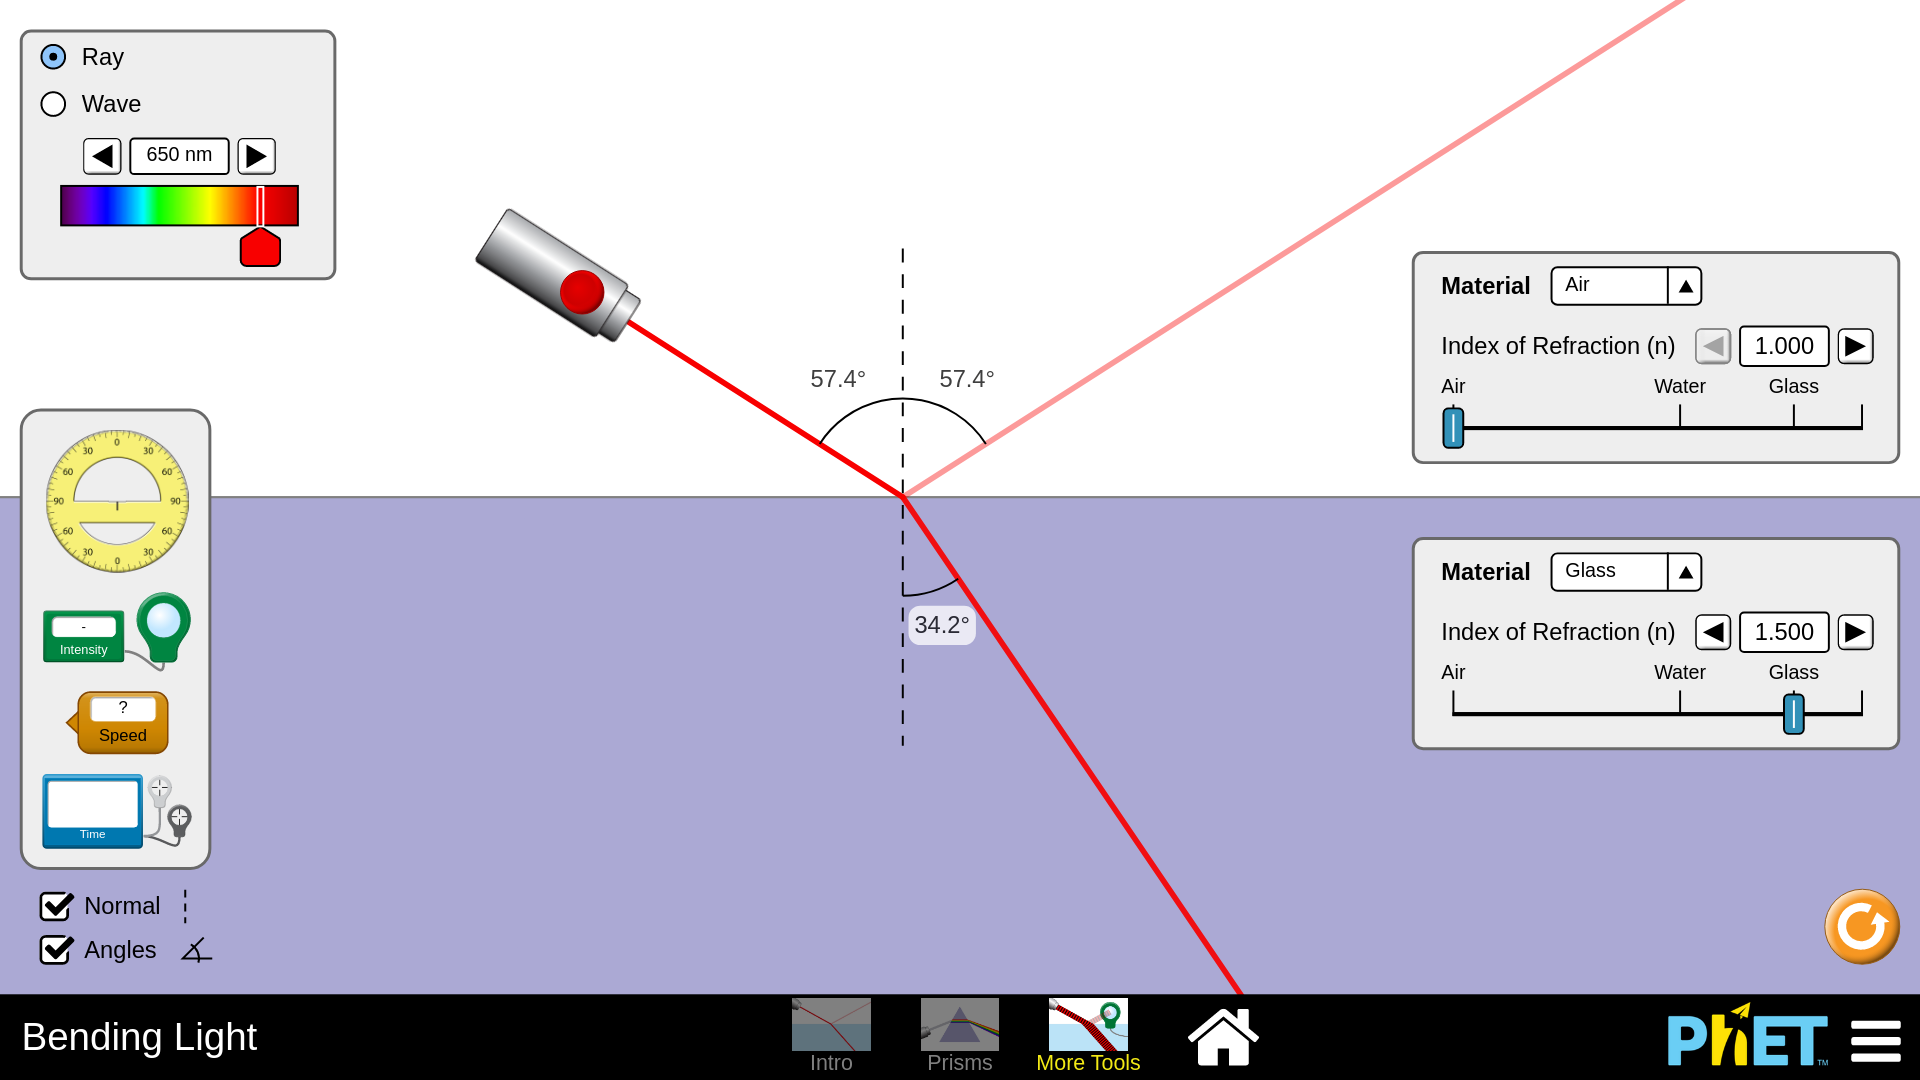
\includegraphics[width=.45\textwidth]{img/phet-1.png}
        }\hfill
        \subfloat[\label{fig:phet-2}]{
            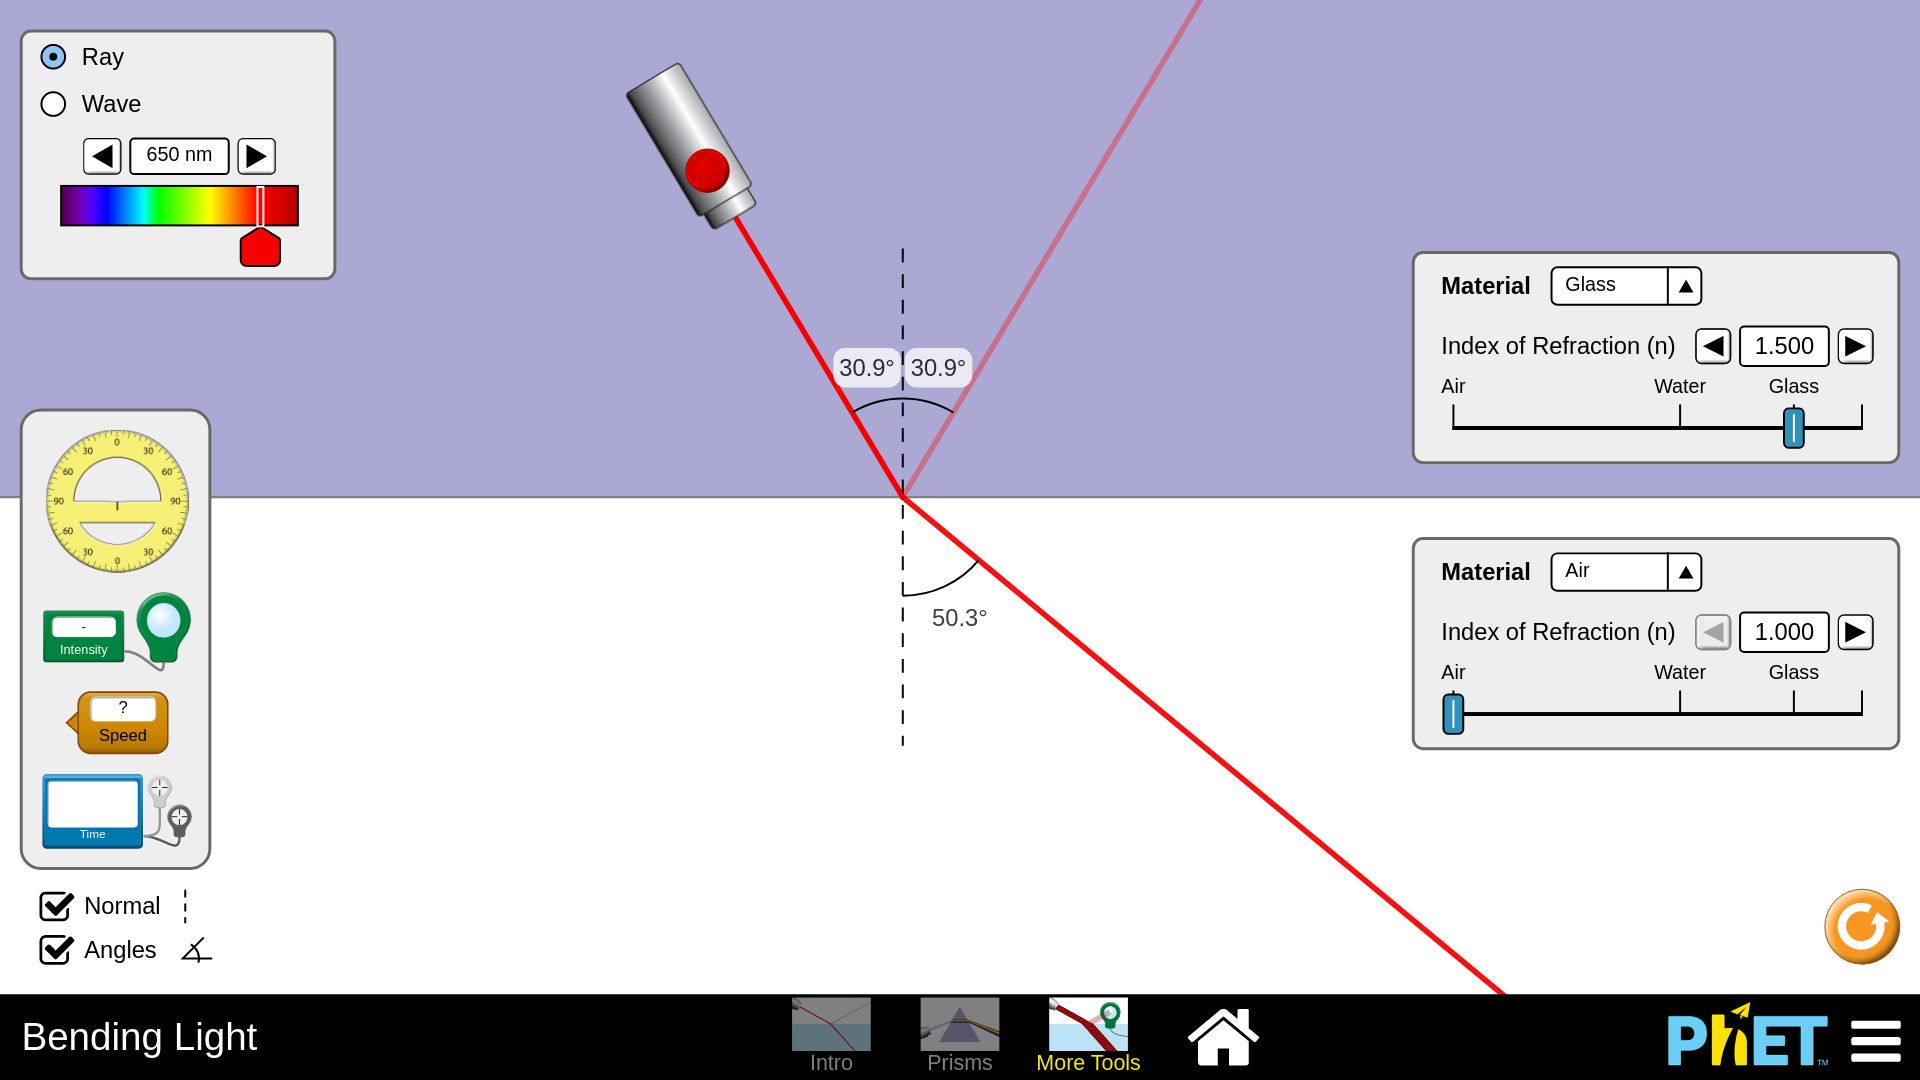
\includegraphics[width=.45\textwidth]{img/phet-2.png}
        }        
        \caption{Simulação \emph{Phet} em (a), feixe luminoso partindo do ar para o vidro, raio refratado aproxima-se da normal ao ponto de contato e em (b), feixe luminoso partindo do vidro para o ar, raio refratado afasta-se da normal ao ponto de contato.}
        \label{fig:phet-a}
    \end{figure}
    \vspace*{10pt}

    Recorda-los que foi associada esta mudança de trajetória que a luz faz, com a mudança na sua velocidade de propagação em cada meio.

    Recorda-los ainda, da previsão newtoniana para a velocidade da luz, nos casos em que a mudança de meios ocorre do ar para água, expressa pela relação

    \begin{align}
        v_{0}<v_{f}
    \end{align}
    em que $v_0$ é a velocidade da luz no ar e $v_f$ é a velocidade da luz na água (ou em qualquer outro meio mais denso).
% Segundo os autores é nessa etapa que se apresentam questões
% e/ou situações para discussão com os alunos, visando relacionar o estudo de um conteúdo com
% situações reais que eles conhecem e presenciam, mas que não conseguem interpretar completa ou
% corretamente porque provavelmente não dispõem de conhecimentos científicos suficientes. Ou seja,
% é na problematização que se deseja aguçar explicações contraditórias e localizar as possíveis
% limitações do conhecimento que vem sendo expressado, quando este é cotejado com o conhecimento
% científico que já foi selecionado para ser abordado (Delizoicov, Angotti e Pernambuco, 2002, p. 201).
% Portanto, esse primeiro momento é caracterizado pela compreensão e apreensão da posição dos alunos
% frente ao tema. É desejável ainda, que a postura do professor se volte mais para questionar e lançar
% dúvidas sobre o assunto que para responder e fornecer explicações.
    \newpage
    \bigskip{}
    \noindent\emph{2º Momento:} Organização do Conhecimento
    \par\noindent\rule{.3\textwidth}{.5pt}  
    \par\noindent\textbf{Tempo previsto:} 20 minutos
    \smallskip
    \par\noindent\textbf{Dinâmica:} Construir a dedução de forma dialogada usando o esquema representativo da \autoref{fig:snell-deducao}
    
    \vspace{10pt}
    \begin{figure}[!ht]        
        \centering              
        \subfloat[\label{fig:snell-deducao-a}]{
            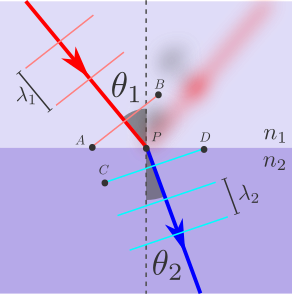
\includegraphics[width=.4\textwidth]{img/snell-1.png}
        }\hspace{20pt}
        \subfloat[\label{fig:snell-deducao-b}]{
            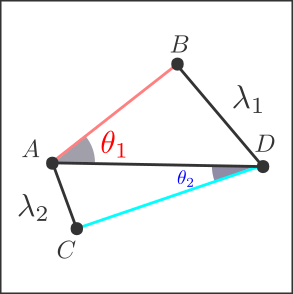
\includegraphics[width=.4\textwidth]{img/snell-2.png}
        }        
        \caption{Esquema representativo da lei de Snell, em (a) as frentes de onda incidente estão representadas por retas paralelas a direção de propagação da onda representada em vermelho, já as frentes de onda em azul representam a parte da onda refrata no material. Em (b) os triângulos $\triangle ABD$ e $\triangle ACD$ formados pelas frentes de onda incidente, refratada e a superfície do meio, são semelhantes.}
        \label{fig:snell-deducao}
  \end{figure}        
  \vspace*{10pt}

  Com o auxílio das figuras acima, extrair a relação
  \begin{align}
  \label{eq:snell-comprimento-de-onda}
      \frac{\sin\theta_1}{\sin\theta_2}&=\frac{\lambda_1}{\lambda_2}
  \end{align}
  Interpretar a eq. \eqref{eq:snell-comprimento-de-onda} em conjunto com os alunos e questioná-los o que se espera que ocorra com os comprimentos de onda $\lambda_1$ e $\lambda_2$ quando $\theta_1<\theta_2$ \emph{(fenômeno de dispersão)}.

  Relacionar a dispersão com os fenômenos da formação do arco-íris e da decomposição da luz branca no prisma de Newton.

    

% Delizoicov e Angotti (1990, p. 29) explicam que nesse
% segundo momento os conhecimentos de Física necessários para a compreensão do tema e da
% problematização inicial devem ser sistematicamente estudados sob orientação do professor.
% Definições, conceitos, relações, leis, apresentadas no texto introdutório, serão agora aprofundados.
% De acordo com Albuquerque, Santos e Ferreira (2015, p. 467) esse é o momento em que os
% conhecimentos científicos passam a ser incorporados nas discussões. Os alunos começam a
% desenvolver uma compreensão a respeito da problematização ou situação inicial. Entretanto, para que
% isso ocorra, materiais devem ser consultados e atividades devem ser sugeridas para complementar as
% discussões, no sentido de incentivar e melhorar a sistematização dos conhecimentos.
% Nessa perspectiva, Delizoicov e Angotti (1990) vêm ressaltar a importância de diversificadas
% atividades, com as quais se poderá trabalhar para organizar a aprendizagem. Sugerem exposições,
% pelo professor, de definições e propriedades, além de formulações de questões (exercícios de fixação
% como dos livros didáticos), textos e experiências. Neste sentido, atualmente poderíamos acrescentar
% as mídias tecnológicas, como televisão, vídeos, filmes, programas tecnológicos, aplicativos de
% celulares, simulações, entre outros, de modo a auxiliar no processo da sistematização do
% conhecimento.
    \newpage
    \bigskip
    \noindent\emph{3º Momento:} Aplicação do Conhecimento
    \par\noindent\rule{.3\textwidth}{.5pt}  
    \par\noindent\textbf{Tempo previsto:} 15 minutos
    \smallskip
    \par\noindent\textbf{Dinâmica:} Iniciar esta parte da aula relembrando a relação que foi encontrada para a velocidade de uma onda qualquer na aula 004
    \begin{align}
        v&=\lambda f
    \end{align}
    a partir da equação acima, obter $\lambda=v/f$ e substituir na \eqref{eq:snell-comprimento-de-onda} ficando com
    \begin{align}
    \label{eq:lei-de-snell-velocidades}
        \frac{\sin\theta_1}{\sin\theta_2}&=\frac{v_1}{v_2}
    \end{align}
    Questionar a relação entre $v_1$ e $v_2$ se $\theta_1>\theta_2$

    Finalizar a aula pedindo para que comparem este resultado com o que obtivemos na teoria corpuscular e ajustar a \eqref{eq:lei-de-snell-velocidades} para a sua forma usual dada por
    \begin{align}
        n_1\sin\theta_1&=n_2\sin\theta_2
    \end{align}
    em que os índices de refração absolutos de cada meio é $n_1=c/v_1$ e $n_2=c/v_2$.
    

% Essa última etapa aborda sistematicamente o
% conhecimento que vem sendo incorporado pelo aluno para analisar e interpretar tanto a situações
% iniciais que determinaram o seu estudo, como outras situações que não estejam diretamente ligadas
% ao motivo inicial, mas que são explicadas pelo mesmo conhecimento. (Delizoicov e Angotti, 1990,
% p. 31).
% Este é o momento importante para que os alunos encontrem relações entre os temas
% abordados, não apenas através dos conceitos, mas também de fenômenos que possam ter alguma
% conexão com as informações apresentadas. No entanto, o professor mantém a postura
% problematizadora, podendo trazer questionamentos que não foram levantados pelos alunos, como
% informações e problemas que surgiram do decorrer dos momentos. Além disso, este é um bom
% momento para o professor formalizar alguns conceitos que não foram aprofundados pelos alunos.
% (Albuquerque, Santos e Ferreira, 2015).

%-----------------------------------------------%
% FIM do plano de aula
%-----------------------------------------------%
    \newpage
    %-----------------------------------------------%
% Início do plano de aula
%-----------------------------------------------%
\thispagestyle{empty}
\begin{center}
	\begin{minipage}[!]{\linewidth}
        \begin{minipage}[!]{.19\linewidth}
            
\includegraphics[width=\linewidth]{img/logo.png}           
        \end{minipage}
        \begin{minipage}[!]{.8\linewidth}
            \center
            \ABNTEXchapterfont\normalsize\MakeUppercase{\imprimirinstituicao}
            \par
            \vspace*{10pt}                     
            \ABNTEXchapterfont\normalsize\MakeUppercase{\centro}
            \par
            \vspace*{10pt}           
            \ABNTEXchapterfont\normalsize\MakeUppercase{\disciplina}
        \end{minipage}        
    \end{minipage}
    \\ \vspace{0.5cm}
    \rule{\textwidth}{.5pt}   
\end{center}
    \textual
    \begin{center}
      \section{Fenômenos Ondulatórios I}
      \par
    \end{center}
    
    \noindent \textbf{Estagiário(a): }\imprimirautor 
    
    \noindent \textbf{U.E.: }EEB Giovani Pasqualini Faraco
    
    \noindent \textbf{Série: }2º Ano\hfill{}\textbf{Turma: }2º--5
    
    \noindent \textbf{Aula:} 007\hfill{}\textbf{Data:} 11/11/2022\hfill{}\textbf{Duração:} $45\min$
    \rule{\textwidth}{.5pt}
    \bigskip{}  
    

    \noindent
    \begin{center}
      \textbf{Interferência, difração e ressonância}
    \par\end{center}
    \vspace{20pt}
    \noindent \textbf{Resumo da aula:} Nesta aula apresentaremos de início, os argumentos fundamentais para a aceitação do modelo ondulatório da luz. Veremos que esta atribuição recebe ainda mais força após estabelecida a teoria eletromagnética de Maxwell, na sequência mostraremos, por meio de vídeos, os fenômenos ondulatórios relacionados a ressonância de ondas mecânicas e posteriormente apresentaremos o experimento de Hertz.
    \smallskip
    \par\noindent \textbf{Habilidades BNCC:} EM13CNT201.
    \medskip
    \subsection*{Objetivo de Aprendizagem}
    \begin{itemize}
        \item Conhecer exemplos do fenômeno de ressonância de ondas mecânicas e eletromagnéticas;
        \item Compreender o principal argumento a favor da concepção da luz como uma onda eletromagnética;
        \item Perceber as diversas formas de construção do conhecimento científico.
    \end{itemize}    
    \bigskip{}    
    \noindent \textbf{Núcleo Conceitual:} \emph{Fenômenos ondulatórios; luz como uma onda eletromagnética; experimento de Hertz.}
    \newpage
    

    \section*{Procedimento Didático} 
    \noindent\emph{1º Momento:} A Problemática da Aceitação Inicial de um Novo Modelo Científico
    \par\noindent\rule{.3\textwidth}{.5pt}  
    \par\noindent\textbf{Tempo previsto:} 10 minutos
    \smallskip
    \par\noindent\textbf{Dinâmica:} Iniciar comentando os resultados obtidos na aula anterior pela Lei de Snell. Perguntar se com o que foi visto até agora é possível fazer alguma afirmação para a natureza da luz, no que concerne ela pertencer ou não a algum dos modelos vistos.
    
    
    Citar que não havia, no entanto nenhuma comprovação experimental que denunciasse de fato a real natureza da luz. E que por mero prestígio devotado à figura de Newton, a teoria corpuscular segue sendo aceita como a descrição "correta" para os fenômenos luminosos, isto deixa o modelo ondulatório "silenciado" por cerca de 200 anos, até que Young quebra este silêncio com o experimento de fenda dupla.

    Iniciar a sequência de slides




% Segundo os autores é nessa etapa que se apresentam questões
% e/ou situações para discussão com os alunos, visando relacionar o estudo de um conteúdo com
% situações reais que eles conhecem e presenciam, mas que não conseguem interpretar completa ou
% corretamente porque provavelmente não dispõem de conhecimentos científicos suficientes. Ou seja,
% é na problematização que se deseja aguçar explicações contraditórias e localizar as possíveis
% limitações do conhecimento que vem sendo expressado, quando este é cotejado com o conhecimento
% científico que já foi selecionado para ser abordado (Delizoicov, Angotti e Pernambuco, 2002, p. 201).
% Portanto, esse primeiro momento é caracterizado pela compreensão e apreensão da posição dos alunos
% frente ao tema. É desejável ainda, que a postura do professor se volte mais para questionar e lançar
% dúvidas sobre o assunto que para responder e fornecer explicações.

    \bigskip{}
    \noindent\emph{2º Momento:} Organização do Conhecimento
    \par\noindent\rule{.3\textwidth}{.5pt}  
    \par\noindent\textbf{Tempo previsto:} 15 minutos
    \smallskip
    \par\noindent\textbf{Dinâmica:} Usando a sequência de slides, explicar o experimento de fenda dupla conduzido por Young e introduzir o conceito de interferência construtiva e destrutiva. Explicar também a difração por um orifício o que permitiu a Young obter, naquela época, dois feixes de luz coerentes entre si.  
    

    \noindent\textbf{Embasamento para os Slides}
    O experimento de fenda dupla, traz uma comprovação da luz como uma onda, haja visto que não há forma alguma de adequar este fenômeno dentro do modelo corpuscular, no entanto, abre-se uma nova questão -- \emph{se a luz é uma onda, que tipo de onda ela é?} Todas as ondas conhecidas até então, estavam enquadradas no escopo das ondas mecânicas governadas pelas leis de Newton, convém mencionar que para a época, uma das características primordiais das ondas de quaisquer natureza, é a necessidade de um meio físico para se propagar, como só se conheciam ondas de natureza mecânica, estes meios geralmente eram o ar, água, terra, cordas, molas e etc. 

    Paralelamente, especulações sobre a velocidade da luz tem sido feita desde os gregos, mas somente por volta do ano de 1670, Ole RØmer obteve um valor para esta velocidade ($c=212\kmps$) baseado em observações dos eclipses das luas de Júpiter. Após RØmer, Fizeau, desta vez experimentalmente, também obtém um valor para a velocidade da luz o que em 1849 Focault, com excelente precisão para a época, atualiza os resultados de Fizeau demonstrando que $c=298\kmps$.

    Ao mesmo tempo em que se desenvolvia técnicas mais precisas para medir a velocidade da Luz, uma teoria para o eletromagnetismo também ia ganhando espaço com James Clerk Maxwell. No desenvolvimento do eletromagnetismo, Maxwell previu a existência de um tipo de onda tal que a velocidade de propagação desta onda, coincide em alto grau com o valor da velocidade da luz obtida pelos experimentos mais precisos da época, no entanto, o eletromagnetismo recém teorizado carecia de comprovação. Fato dado por Heinrich Hertz em 1883.

    A importância dos experimentos de Hertz para o Eletromagnetismo de Maxwell, não apenas comprova experimentalmente a existência das ondas eletromagnéticas como também torna possível a inferência da luz visível como uma classe deste tipo de onda, o próprio Maxwell afirma em 1862 que:

    \begin{citacao}
        ``A velocidade das ondas transversais em nosso meio hipotético, calculada a partir dos experimentos electromagnéticos dos Srs. Kolhrausch e Weber, concorda tão exatamente com a velocidade da luz, calculada pelos experimentos óticos do Sr. Fizeau, que é difícil evitar a inferência de que a luz consiste nas ondulações transversais do mesmo meio que é a causa dos fenômenos elétricos e magnéticos.'' \cite{NUSSENZVEIG31997}
    \end{citacao}

    % https://www.youtube.com/watch?v=jUHgIYNEzJQ

    % https://cref.if.ufrgs.br/?contact-pergunta=leis-de-maxwell-e-ondas-eletromagneticas

    % https://cref.if.ufrgs.br/?contact-pergunta=como-a-luz-viaja-a-300-000-kms

    % https://cref.if.ufrgs.br/?contact-pergunta=leis-de-maxwell-e-ondas-eletromagneticas

    % http://www.virtual.ufc.br/solar/aula_link/SOLAR_2/Curso_de_Graduacao_a_Distancia/LFIS/A_a_H/Fisica_IV/aula_04/01.html

% Delizoicov e Angotti (1990, p. 29) explicam que nesse
% segundo momento os conhecimentos de Física necessários para a compreensão do tema e da
% problematização inicial devem ser sistematicamente estudados sob orientação do professor.
% Definições, conceitos, relações, leis, apresentadas no texto introdutório, serão agora aprofundados.
% De acordo com Albuquerque, Santos e Ferreira (2015, p. 467) esse é o momento em que os
% conhecimentos científicos passam a ser incorporados nas discussões. Os alunos começam a
% desenvolver uma compreensão a respeito da problematização ou situação inicial. Entretanto, para que
% isso ocorra, materiais devem ser consultados e atividades devem ser sugeridas para complementar as
% discussões, no sentido de incentivar e melhorar a sistematização dos conhecimentos.
% Nessa perspectiva, Delizoicov e Angotti (1990) vêm ressaltar a importância de diversificadas
% atividades, com as quais se poderá trabalhar para organizar a aprendizagem. Sugerem exposições,
% pelo professor, de definições e propriedades, além de formulações de questões (exercícios de fixação
% como dos livros didáticos), textos e experiências. Neste sentido, atualmente poderíamos acrescentar
% as mídias tecnológicas, como televisão, vídeos, filmes, programas tecnológicos, aplicativos de
% celulares, simulações, entre outros, de modo a auxiliar no processo da sistematização do
% conhecimento.

    \bigskip
    \noindent\emph{3º Momento:} Aplicação do Conhecimento
    \par\noindent\rule{.3\textwidth}{.5pt}  
    \par\noindent\textbf{Tempo previsto:} 20 minutos
    \smallskip
    \par\noindent\textbf{Dinâmica:} Apresentar os fenômeno de ressonância, por meio dos vídeos. Os dois primeiros vídeos abordam exemplos bem conhecidos sobre este fenômeno, a ressonância de ondas sonoras numa taça de cristal (Figura --\autoref{fig:ressonancia-cristal}) e a queda da ponte de Tacoma (Figura --\autoref{fig:ressonancia-tacoma}).

    \vspace{10pt}
    \begin{figure}[!ht]        
        \centering              
        \subfloat[\label{fig:ressonancia-cristal}]{
            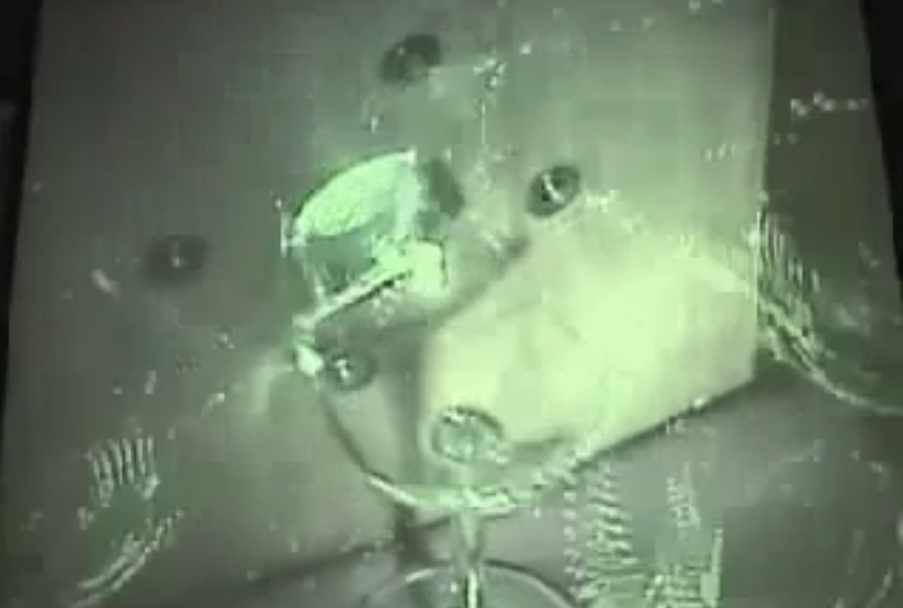
\includegraphics[width=.4\textwidth]{img/ressonancia-cristal.png}
        }\hspace{20pt}
        \subfloat[\label{fig:ressonancia-tacoma}]{
            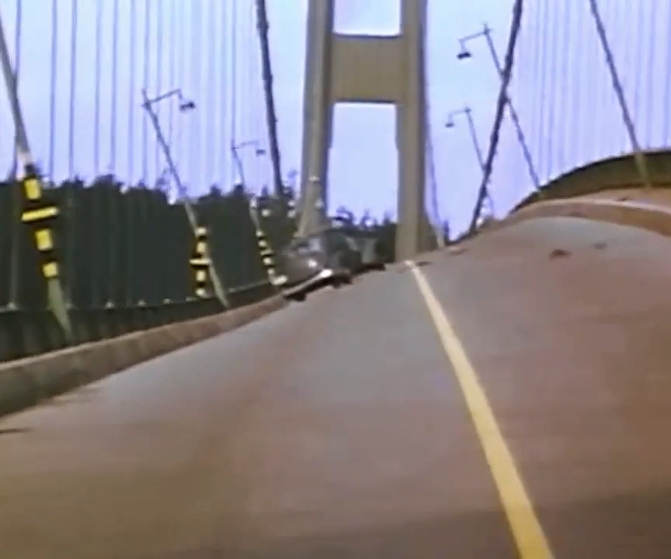
\includegraphics[width=.4\textwidth]{img/ressonancia-tacoma.png}
        }        
        \caption{Fenômenos de Ressonância: (a) Ressonância sonora numa taça de cristal ocorrendo segundos após a sua ruptura. (b) O famoso caso da ponte de Tacoma Narrows (1940)}
        \label{fig:ressonancia-1}
    \end{figure}        
    \vspace*{10pt}
    \newpage
    Após apresentar o fenômeno, mostrar o vídeo da ressonância em diapasões (Figura -- \autoref{fig:ressonancia-diapasoes}) o experimento deste vídeo é análogo ao experimento de Hertz (Figura -- \autoref{fig:ressonancia-hertz}) para as ondas eletromagnéticas.    
    \vspace{10pt}
    \begin{figure}[!ht]        
        \centering              
        \subfloat[\label{fig:ressonancia-diapasoes}]{
            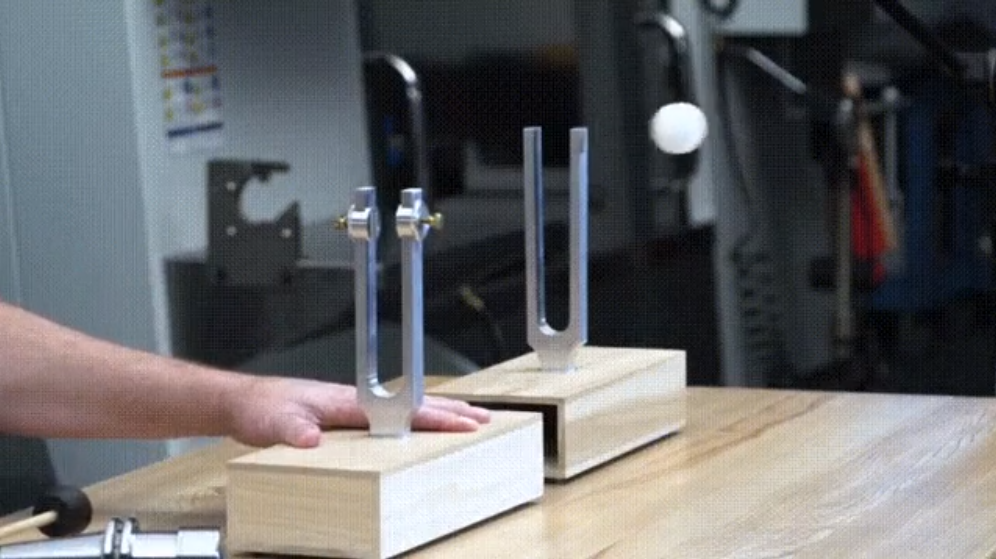
\includegraphics[width=.4\textwidth]{img/ressonancia-diapasao.png}
        }\hspace{20pt}
        \subfloat[\label{fig:ressonancia-hertz}]{
            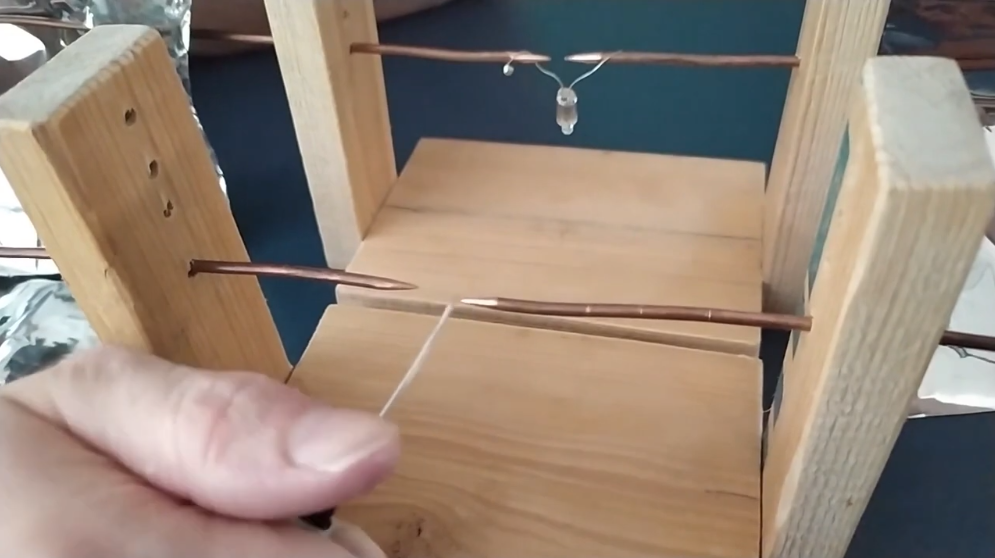
\includegraphics[width=.4\textwidth]{img/ressonancia-hertz.png}
        }        
        \caption{Fenômenos de Ressonância: (a) Ressonância sonora em diapasões. (b) Reprodução do experimento de Hertz}
        \label{fig:ressonancia-2}
    \end{figure}        
    \vspace*{10pt}

    Apresentar o experimento de Hertz como análogo ao fenômeno de ressonância entre diapasões.

    Questionar se conseguem encontrar alguma aplicação no cotidiano que se beneficie dos fenômenos de ressonância \emph{(transmissão de informações via ondas de radiofrequências; wi-fi; bluetooth; ressonância magnética e etc)}.

    Recuperar a aula enfatizando o que foi visto no vídeo do experimento de Hertz e realçar o caráter comprobatório dada ao experimento para adequar a luz como onda eletromagnética pela inferência da similaridade entre as velocidades destas ondas.
    

% Essa última etapa aborda sistematicamente o
% conhecimento que vem sendo incorporado pelo aluno para analisar e interpretar tanto a situações
% iniciais que determinaram o seu estudo, como outras situações que não estejam diretamente ligadas
% ao motivo inicial, mas que são explicadas pelo mesmo conhecimento. (Delizoicov e Angotti, 1990,
% p. 31).
% Este é o momento importante para que os alunos encontrem relações entre os temas
% abordados, não apenas através dos conceitos, mas também de fenômenos que possam ter alguma
% conexão com as informações apresentadas. No entanto, o professor mantém a postura
% problematizadora, podendo trazer questionamentos que não foram levantados pelos alunos, como
% informações e problemas que surgiram do decorrer dos momentos. Além disso, este é um bom
% momento para o professor formalizar alguns conceitos que não foram aprofundados pelos alunos.
% (Albuquerque, Santos e Ferreira, 2015).

%-----------------------------------------------%
% FIM do plano de aula
%-----------------------------------------------%
    \newpage
    %-----------------------------------------------%
% Início do plano de aula
%-----------------------------------------------%
\thispagestyle{empty}
\begin{center}
	\begin{minipage}[!]{\linewidth}
        \begin{minipage}[!]{.19\linewidth}
            
\includegraphics[width=\linewidth]{img/logo.png}           
        \end{minipage}
        \begin{minipage}[!]{.8\linewidth}
            \center
            \ABNTEXchapterfont\normalsize\MakeUppercase{\imprimirinstituicao}
            \par
            \vspace*{10pt}                     
            \ABNTEXchapterfont\normalsize\MakeUppercase{\centro}
            \par
            \vspace*{10pt}           
            \ABNTEXchapterfont\normalsize\MakeUppercase{\disciplina}
        \end{minipage}        
    \end{minipage}
    \\ \vspace{0.5cm}
    \rule{\textwidth}{.5pt}   
\end{center}
    \textual
    \begin{center}
      \section{A Teoria Éter}
      \par
    \end{center}
    
    \noindent \textbf{Estagiário(a): }\imprimirautor 
    
    \noindent \textbf{U.E.: }EEB Giovani Pasqualini Faraco
    
    \noindent \textbf{Série: }2º Ano\hfill{}\textbf{Turma: }2º--5
    
    \noindent \textbf{Aula:} 008\hfill{}\textbf{Data:} 04/11/2022\hfill{}\textbf{Duração:} $45\min$
    \rule{\textwidth}{.5pt}
    \bigskip{}  
    

    \noindent
    \begin{center}
      \textbf{Qual o meio de propagação da luz?}
    \par\end{center}
    \smallskip{}
    \noindent \textbf{Resumo da aula:} Será dado inicio a uma discussão a cerca de qual meio deve dar suporte às onda eletromagnéticas e consequentemente aos fenômenos luminosos.
    \medskip{}
    \par\noindent \textbf{Habilidades BNCC:} EM13CNT201.
    \bigskip{}
    \subsection*{Objetivo de Aprendizagem}
    \begin{itemize}
        \item Justificar a necessidade da Teoria do Éter na época do desenvolvimento da teoria eletromagnética;
        \item Exemplificar a transitoriedade das questões científicas, no que concerne ao levantamento contínuo de hipóteses cada vez mais elaboradas em decorrência da construção do conhecimento.
    \end{itemize}    
    \smallskip{}    
    \noindent \textbf{Núcleo Conceitual:} \emph{Luz como uma onda eletromagnética; a necessidade do Éter.}
    \newpage
    

    \section*{Procedimento Didático} 
    \noindent\emph{1º Momento:} Breve Revisão
    \par\noindent\rule{.3\textwidth}{.5pt}  
    \par\noindent\textbf{Tempo previsto:} 10 minutos
    \smallskip
    \par\noindent\textbf{Dinâmica:} Retomando o que foi discutido na última aula, o professor segue investigando os fenômenos luminosos que só podem ser explicados, se a luz for concebida como uma onda, inicia sua sua fala recapitulando o que foi visto na sequência:

    \begin{itemize}
        \item Vimos que há dois modelos contraditórios para descrever os fenômenos luminosos, o modelo corpuscular e o modelo ondulatório;
        \item Vimos que no modelo corpuscular:
        \begin{itemize}
            \item A luz é composta por minúsculas partículas de luz;
            \item O fenômeno de reflexão é compreendido pela lei da conservação do momento linear;
            \item O ângulo de reflexão concorda com as observações e é igual ao ângulo de incidência;
            \item A velocidade da luz na reflexão é igual a velocidade de incidência, apenas trocando-se a direção da  componente vertical da velocidade;
            \item O fenômeno de refração é compreendido pela segunda lei de newton, que prevê a existência de uma força que altera somente a componente vertical da velocidade;
            \item A velocidade da luz em meios mais densos é maior;
            \item Alguns fenômenos seguem sem compreensão como: os fenômenos de interferência, difração e etc
        \end{itemize}
        \item Já no modelo ondulatório:
        \begin{itemize}
            \item A luz é concebida como uma onda que se propaga em algum meio [este meio será problematizado ao final desta aula];
            \item Os fenômenos de reflexão e refração são compreendidos pelo princípio de Hyugens, bem como todos os fenômenos de propagação;
            \item O ângulo de incidência e reflexão são iguais e são descritos pela lei de Snell-Descartes;
            \item A lei de Snell-Descartes também descreve o fenômeno de refração;
            \item A velocidade da luz em meios mais densos é menor;
            \item Fenômenos de interferência e difração são explicados pelo princípio de Huygens e observados no experimento de Young;
            \item Os experimentos de Young, também comprovam a que a luz é um tipo de onda;
            \item O fenômeno de ressonância de ondas eletromagnéticas demonstrados por Hertz, somado às medições obtidas para a velocidade da luz e em combinado com o desenvolvimento do eletromagnetismo, sugerem que a luz seja um tipo de onda eletromagnética de velocidade conhecida por $c=\sim 298\kmps$.
        \end{itemize}
    \end{itemize}

    Feita esta revisão inicial, problematizar da seguinte forma: \emph{Muito bem, o que temos? Com Young  nós temos uma comprovação de que a luz é uma onda e com Maxwell que essa onda é a onda eletromagnética. Sabe-se que toda onda precisa de um meio para se propagar, então que meio é esse? Alguma hipótese?} Anotar as hipóteses no quadro.
    

% Segundo os autores é nessa etapa que se apresentam questões
% e/ou situações para discussão com os alunos, visando relacionar o estudo de um conteúdo com
% situações reais que eles conhecem e presenciam, mas que não conseguem interpretar completa ou
% corretamente porque provavelmente não dispõem de conhecimentos científicos suficientes. Ou seja,
% é na problematização que se deseja aguçar explicações contraditórias e localizar as possíveis
% limitações do conhecimento que vem sendo expressado, quando este é cotejado com o conhecimento
% científico que já foi selecionado para ser abordado (Delizoicov, Angotti e Pernambuco, 2002, p. 201).
% Portanto, esse primeiro momento é caracterizado pela compreensão e apreensão da posição dos alunos
% frente ao tema. É desejável ainda, que a postura do professor se volte mais para questionar e lançar
% dúvidas sobre o assunto que para responder e fornecer explicações.

    \bigskip{}
    \noindent\emph{2º Momento:} Organização do Conhecimento
    \par\noindent\rule{.3\textwidth}{.5pt}  
    \par\noindent\textbf{Tempo previsto:} 20 minutos
    \smallskip
    \par\noindent\textbf{Dinâmica:} Nesta parte o professor deve problematizar cada hipótese forçando-os ao pensamento da época de Maxwell e seus contemporâneos. Para refutar as respostas dos estudantes, podemos nos embasar da seguinte forma:

    \begin{itemize}
        \item A hipótese mais óbvia é que a luz tem como meio de propagação o ar, porém esta hipótese é facilmente refutada. A título de exemplo, pode-se argumentar que o som é uma onda que se propaga pelo ar, mas não se propaga no vácuo, no entanto a luz que sai do sol chega até nós mesmo não havendo ar entre o Sol e a Terra.
        \item Qualquer outra hipótese que se utilize de meios mecânicos para justificar o meio de propagação das ondas luminosas, deve ser refutada pelos mesmos argumentos acima.
        \item Outra hipótese que pode surgir é o vácuo como um meio de propagação da luz, porém o vácuo não era concebível à época, além do mais o vácuo não é um meio propriamente dito e sim, talvez, a ausência de um, neste caso, o vácuo é antes um problema do que uma solução. 
    \end{itemize}

    Manter a discussão até se tenha um consenso de que é necessário haver algum meio "especial" cujo o qual dê suporte a propagação das ondas eletromagnéticas.
    

% Delizoicov e Angotti (1990, p. 29) explicam que nesse
% segundo momento os conhecimentos de Física necessários para a compreensão do tema e da
% problematização inicial devem ser sistematicamente estudados sob orientação do professor.
% Definições, conceitos, relações, leis, apresentadas no texto introdutório, serão agora aprofundados.
% De acordo com Albuquerque, Santos e Ferreira (2015, p. 467) esse é o momento em que os
% conhecimentos científicos passam a ser incorporados nas discussões. Os alunos começam a
% desenvolver uma compreensão a respeito da problematização ou situação inicial. Entretanto, para que
% isso ocorra, materiais devem ser consultados e atividades devem ser sugeridas para complementar as
% discussões, no sentido de incentivar e melhorar a sistematização dos conhecimentos.
% Nessa perspectiva, Delizoicov e Angotti (1990) vêm ressaltar a importância de diversificadas
% atividades, com as quais se poderá trabalhar para organizar a aprendizagem. Sugerem exposições,
% pelo professor, de definições e propriedades, além de formulações de questões (exercícios de fixação
% como dos livros didáticos), textos e experiências. Neste sentido, atualmente poderíamos acrescentar
% as mídias tecnológicas, como televisão, vídeos, filmes, programas tecnológicos, aplicativos de
% celulares, simulações, entre outros, de modo a auxiliar no processo da sistematização do
% conhecimento.
    \newpage
    \bigskip
    \noindent\emph{3º Momento:} Postulado
    \par\noindent\rule{.3\textwidth}{.5pt}  
    \par\noindent\textbf{Tempo previsto:} 10 minutos
    \smallskip
    \par\noindent\textbf{Dinâmica:} Ofertar como alternativa a hipótese do Éter Luminífero

    \begin{itemize}
        \item A hipótese do Éter:
        \item A teoria eletromagnética não definia claramente a partir de qual observador a velocidade da luz estava sendo obtida, postulou-se então o seguinte:
        \begin{itemize}
            \item \emph{Existe um meio privilegiado onde são válidas as leis do eletromagnetismo. Tal meio foi chamado de O Éter luminífero.}
            \item O Éter é um fluído material, porém, imponderável, infinito, homogêneo e isotrópico permeando todos os corpos, inclusive o interior deles.
            \item no interior de corpos transparentes o éter seria parcialmente arrastado pelo corpo quando em movimento em relação ao éter exterior, dito estacionário (Proposição créditada à Fresnel). Quanto aos corpos opacos, o éter se manteria estacionário, sem ser perturbado pelo movimento desses.
            \item O éter deve substituir a ideia de referencial absoluto estabelecida na mecânica newtoniana na descrição dos fenômenos físicos, inclusive no que concerne a descrição da própria mecânica.
        \end{itemize}       
        
    \end{itemize}

       Na próxima aula será continuada as investigações e tentativas de detecção do Éter através do interferômetro de Michelson-Morley.
    

% Essa última etapa aborda sistematicamente o
% conhecimento que vem sendo incorporado pelo aluno para analisar e interpretar tanto a situações
% iniciais que determinaram o seu estudo, como outras situações que não estejam diretamente ligadas
% ao motivo inicial, mas que são explicadas pelo mesmo conhecimento. (Delizoicov e Angotti, 1990,
% p. 31).
% Este é o momento importante para que os alunos encontrem relações entre os temas
% abordados, não apenas através dos conceitos, mas também de fenômenos que possam ter alguma
% conexão com as informações apresentadas. No entanto, o professor mantém a postura
% problematizadora, podendo trazer questionamentos que não foram levantados pelos alunos, como
% informações e problemas que surgiram do decorrer dos momentos. Além disso, este é um bom
% momento para o professor formalizar alguns conceitos que não foram aprofundados pelos alunos.
% (Albuquerque, Santos e Ferreira, 2015).

%-----------------------------------------------%
% FIM do plano de aula
%-----------------------------------------------%


% encionar a unificação da eletricidade com o magnetismo feita por James Clerk Maxwell e publicada em  seus trabalhos no ano de 1873. Neste trabalho, uma das conclusões obtidas por Maxwell foi a existência das ondas eletromagnéticas, desta forma, Maxwell unifica duas áreas distintas da Física: a Eletricidade e o Magnetismo, formando o que chamamos hoje de Eletromagnetismo. Ao calcular a rapidez (velocidade) com a qual a onda eletromagnética se propagaria encontrou um valor consistente com as melhores determinações da velocidade da luz até então (medidas do Fizeau). Cogitou então que a luz pudesse ser uma onda eletromagnética. Em 1862 James Clerk Maxwell afirmou:
    
%     \begin{citacao}
%         ``A velocidade das ondas transversais em nosso meio hipotético, calculada a partir dos experimentos electromagnéticos dos Srs. Kolhrausch e Weber, concorda tão exatamente com a velocidade da luz, calculada pelos experimentos óticos do Sr. Fizeau, que é difícil evitar a inferência de que a luz consiste nas ondulações transversais do mesmo meio que é a causa dos fenômenos elétricos e magnéticos.''
%     \end{citacao}



%     Trabalhos posteriores à Maxwell como os de Hertz (existência das ondas eletromagnéticas), Fizeaul
    
    \chapter{Material de Apoio}
    \label{ape:texto-de-apoio}
    \thispagestyle{empty}
    \begin{center}
    
    \resizebox{!}{.8cm}{
        \textbf{Óptica}        
    }
    \section{Noções de Óptica Ondulatória}
\end{center}
\begin{flushright}
    
     
    \rule{.33\textwidth}{.5pt}
    \renewcommand{\thefootnote}{\fnsymbol{footnote}}
    \par\noindent Por: Rodrigo Nascimento\footnote[2]{Estágio Curricular Obrigatório III -- ESC3003 (UDESC).} 
\end{flushright}


\section*{Introdução}       

O que é a Luz, como se propaga e qual a sua natureza, são os temas centrais da Óptica. Neste módulo de ensino, iremos estudar os aspectos mais elementares da propagação luminosa, que já eram parcialmente conhecidos desde a antiguidade.

A óptica se ramifica em diversas áreas de estudo, no ENEM tem-se basicamente apenas duas ramificações, sendo elas:
\begin{itemize}
    \item \textbf{Óptica Geométrica:} A luz é estudada como raios que percorrem trajetórias retilíneas. Fenômenos como a reflexão e a refração são observados, além disso, estuda-se também a formação de imagens em espelhos e lentes;
    \item \textbf{Óptica Física ou Ondulatória:} A luz é estudada como uma onda, os fenômenos como difração, interferência e polarização também aparecem naturalmente.
\end{itemize}

\setlength\intextsep{-20pt}
\begin{wrapfigure}[5]{l}{0.48\textwidth}
    \centering
    \begin{mybox}[colback=white, colframe=cyan,colbacktitle=cyan!85!cyan,]{Mais sobre!}
        Há diversos vídeos na plataforma YouTube que tratam sobre o tema, um deles pode ser encontrado \href{https://youtu.be/oSUHXeiaQ98}{aqui}.
    \end{mybox}    
\end{wrapfigure}

\noindent Os fenômenos da óptica geométrica, estão de acordo com a \emph{teoria corpuscular da luz}, creditada (erroneamente) à Isaac Newton (1643-1727). Uma segunda teoria, a \emph{teoria ondulatória}, foi proposta principalmente por Christian Huygens (1629-1695), Robert Hooke (1635-1703) e Thomas Young (1773-1829). Estes dois modelos formaram o palco para intensas discussões entre meados dos séculos XVII e XVIII.

A seguir falaremos um pouco sobre o conceito de ondas, para que possamos compreender corretamente os fenômenos luminosos.

\section*{Ondas}
\label{sec:nocoes-basicas-ondas}
Onda é o fenômeno causado pela perturbação de uma região do espaço ou um campo físico, propaga-se através desta uma região, a que chamamos de \emph{meio}, numa determinada velocidade. Um exemplo bastante comum, são as ondas do mar, causadas principalmente pelo deslocamento das massas de ar, propagam-se em direção à costa. Outros exemplos de ondas são: o som, a luz, os sinais de comunicação (rádio, televisão, celular e etc), os terromotos, dentre outros.

\begin{mybox}[colback=white, colframe=amarelo,colbacktitle=amarelo!85!amarelo,]{Conceituando}
    \emph{Uma onda pode ser compreendida como uma "perturbação" que se propaga de um ponto a outro, com velocidade definida.}
\end{mybox}

Neste sentido, fala-se de onda quando essa perturbação ocorre \emph{sem} que haja transporte de matéria, ou seja, em geral ondas só transportam energia!

\subsection*{Tipos de Ondas}
Pode-se classificar as ondas em quatro tipos:
\begin{enumerate}
    \item \textbf{Ondas Mecânicas:} Existem apenas num meio material dependendo dele para se propagar, como exemplo: ondas sonoras, ondas do mar e terremotos.  
    \item \textbf{Ondas Eletromagnéticas:} Não precisam de um meio material para existir ou se propogar, propagam-se tanto no vácuo como em meios materiais são exemplos de ondas eletromagnéticas: luz, microondas, rede wireless, sinal de GPS e etc.
    \item \textbf{Ondas de Matéria:} São mais comuns em laboratórios de pesquisa em Física Quântica e Teoria de Campos, estão associadas ao átomo e suas partículas elementares como: elétron, próton, bósons e etc.
    \item \textbf{Ondas Gravitacionais:} Ondulações geradas por colisões violentas entre corpos celestes, se propagam pelo espaço-tempo.
\end{enumerate}
As ondas ainda podem ser classificadas quanto a sua direção de propagação, sendo elas:
\begin{itemize}
    \item \emph{Unidimensionais:} Propagam-se em apenas uma direção, como por exemplo, as ondas em uma corda.
    \item \emph{Bidimensionais:} Com direção de propagação em um plano ou uma superfície, tal como as ondas num lago ou os terromotos.
    \item \emph{Tridimensionais:} Se propagam em todas as direções, como por exemplo o som e a luz. 
\end{itemize}
E por fim, também podem ser classificadas quanto a direção de vibração ou oscilação, sendo chamadas de:
\begin{itemize}
    \item \emph{Transversais:} Se originadas por oscilações perpendiculares à direção de propagação (ondas no mar, luz e ondas numa corda).
    \item \emph{Longitudinais:} Quando se propagam na mesma direção de oscilação (som).
\end{itemize}
Para o caso da luz, podemos dizer então que:
\begin{mybox}[colback=white, colframe=amarelo,colbacktitle=amarelo!85!amarelo,]{Conceituando}
    \emph{A Luz é uma onda eletromagnética, tridimensional transversal que propaga-se a uma velocidade constante sendo o valor da sua velocidade no vácuo $c=299\;792\;459\mps$ ou, aproximadamente $3,0\times 10^{8}\mps$.}
\end{mybox}

 \subsection*{Comprimento de onda}

Algumas grandezas são fundamentais para a descrição correta da onda, uma delas é o seu \emph{comprimento de onda} representado geralmente pela letra grega \emph{lambda} $\lambda$.

 \setlength\intextsep{-20pt}
 \begin{wrapfigure}[16]{l}{.6\textwidth}
    \centering
    \begin{mybox}[colback=white, colframe=deepred,colbacktitle=deepred!85!deepred,]{Comprimento de Onda ($\lambda$)}
        O \emph{comprimento de onda} $\lambda$ é a distância paralela à direção de propagação da onda, entre repetições da forma da onda.
        \tcblower
        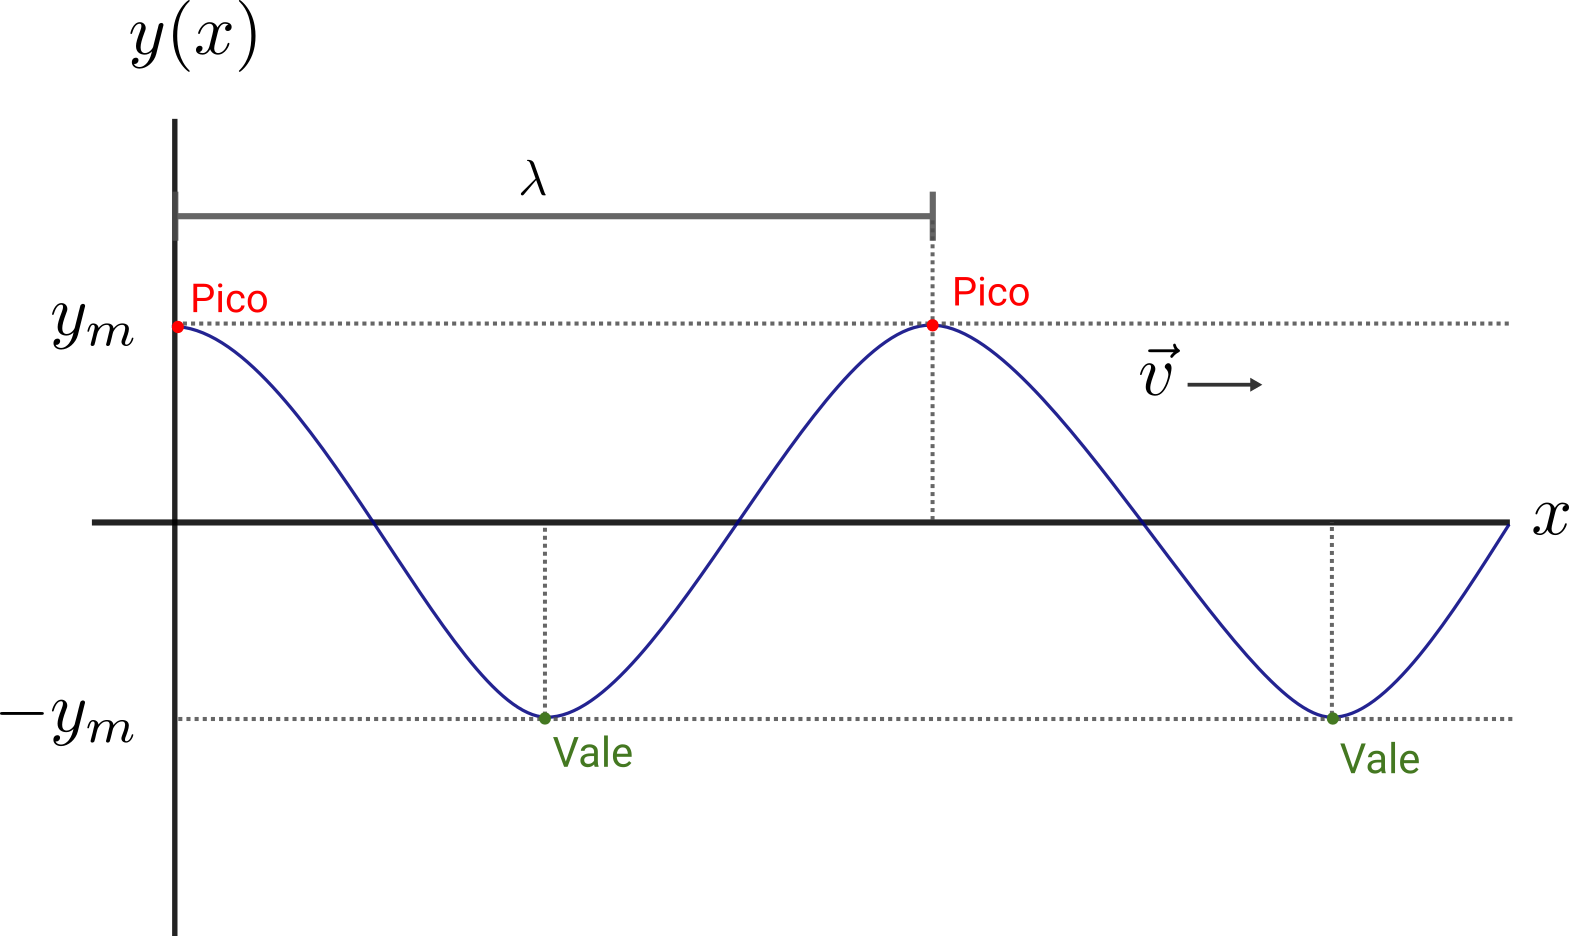
\includegraphics[width=1\textwidth]{img/lambda-1.png}
        \caption{Onda propagando-se em uma corda, paralela à direção do eixo $x$}
        \label{fig:comprimento-onda-corda} 
    \end{mybox}            
 \end{wrapfigure}

\noindent Imagine por exemplo, uma \emph{onda mecânica transversal unidimensional} propagando-se numa corda ao produzirmos alguns pulsos para cima e para baixo.

\noindent A \autoref{fig:comprimento-onda-corda} ilustra aproximadamente o que pode acontece com relação ao formato da onda em função do deslocamento em $x$ das frentes de onda (pulsos) produzidas.

\noindent Os pontos da corda que alcançam os pontos mais altos no eixo $y$ são os \emph{picos}, também chamados de \emph{Amplitude Máxima da Onda} ($y_m$), já os pontos mais baixos os \emph{vales}, são conhecidos como as \emph{Amplitudes Mínimas da Onda} ($-y_m$).

\noindent A distância entre dois picos locais ou (\emph{máximos consecutivos}), é igual a distância entre dois vales locais (\emph{mínimos consecutivos}), a essa medida chamamos de \textbf{comprimento de onda} $\lambda$. Tem unidade de distância (\emph{metro-$\m$, centímetro-$\cm$, nanômetro-$\nm$ e etc}).

       
\subsection*{Período}
\setlength\intextsep{-10pt}
\begin{wrapfigure}[21]{r}{.6\textwidth}
    \centering
    \begin{mybox}[colback=white, colframe=deepred,colbacktitle=deepred!85!deepred,]{Período de uma Onda ($T$)}
        O \emph{período} $T$ de oscilação de uma onda, é o tempo necessário para que a onda complete um ciclo, análogo ao período de oscilação de um pêndulo simples.
        \tcblower
        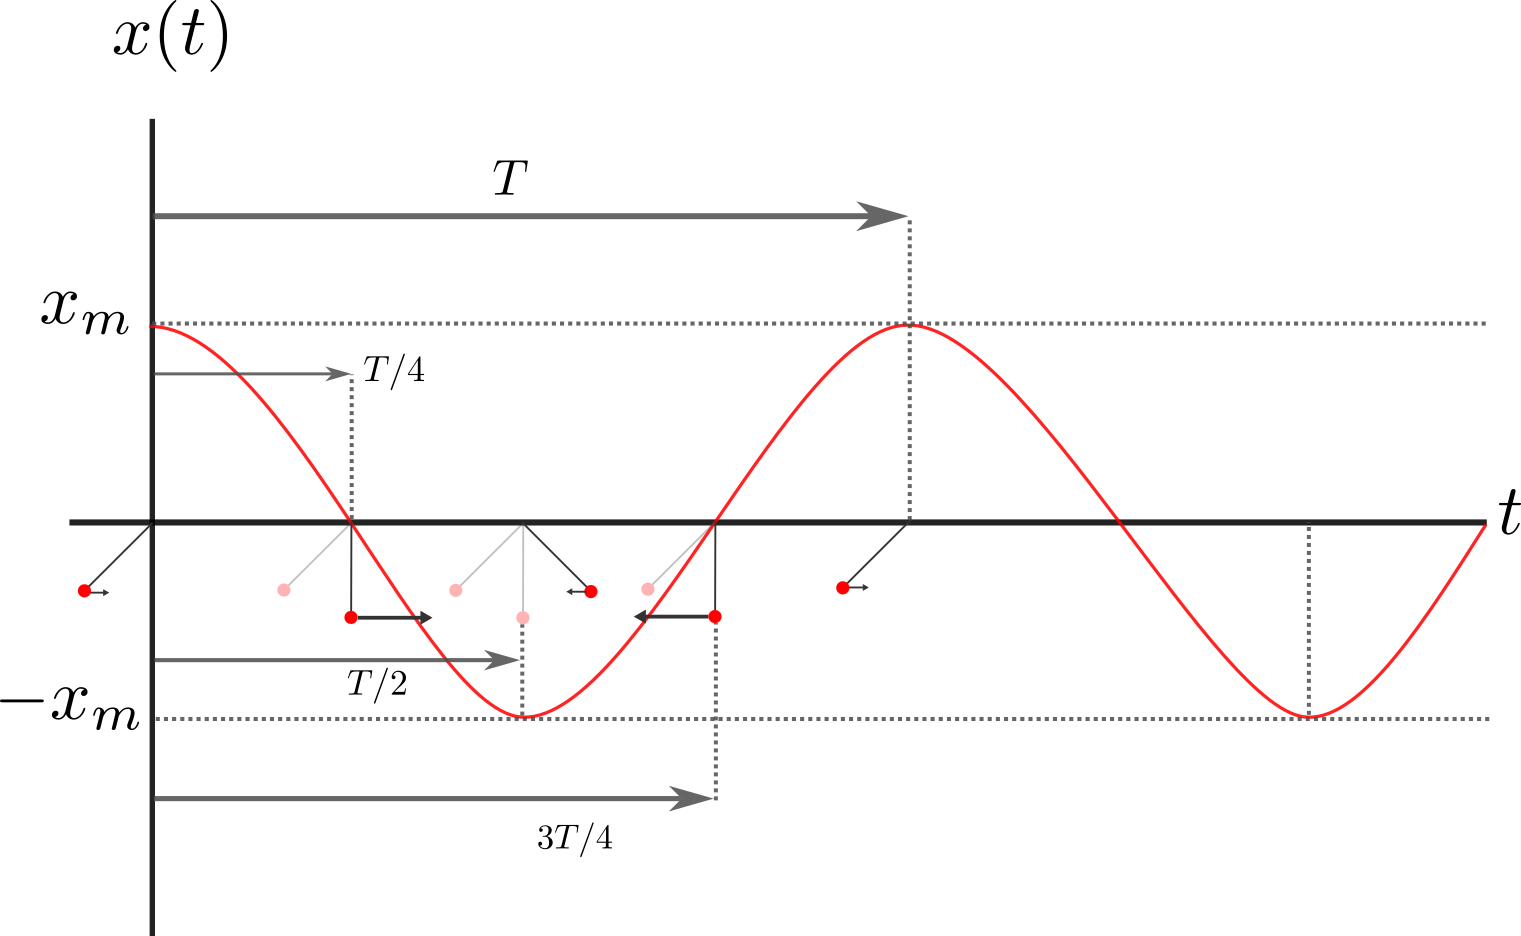
\includegraphics[width=1\textwidth]{img/periodo-1.png}
        \caption{No gráfico $x(t)$, tem-se o esquema de oscilação de um pêndulo que parte de uma posição $x_m$, vai até a posição oposta $-x_m$ e retorna a sua posição inicial.}
        \label{fig:periodo-onda-corda} 
    \end{mybox}            
\end{wrapfigure}       
Outra grandeza fundamental para a descrição de uma onda, é o seu \emph{período de oscilação}, utiliza-se geralmente a letra maiúscula $T$ para representá-lo. Na \autoref{fig:periodo-onda-corda} à direita, representamos o gráfico de um pêndulo oscilando no tempo, supondo que o pêndulo é colocado para oscilar a partir de uma posição qualquer $x_m$, após $T/4$ de tempo ele passa pela sua posição de equilíbrio em $x=0$, vai até a posição extremamente oposta $-x_m$ num tempo $T/2$, passa novamente pela sua posição de equilíbrio num tempo $3T/4$ e retorna ao ponto inicial em $x_m$. Ao tempo total em que o pêndulo fez este percurso, chamamos de \textbf{período de oscilação} $T$. Possui a unidade de tempo (\emph{segundo-$\s$}, \emph{milissegundo}-$\mathrm{ms}$ e etc).

As vezes estamos mais interessados em saber quantos ciclos uma onda conclui em um intervalo de tempo determinado. Por isso, defini-se uma grandeza física que tem uma relação imediata com o período da onda. Essa grandeza é a \emph{frequência da onda} caracterizada pela letra minúscula $f$.

\begin{mybox}[colback=white, colframe=deepred,colbacktitle=deepred!85!deepred,]{Frequência de uma Onda ($f$)}
    A quantidade de oscilações por unidade de tempo que um movimento oscilatório quelaquer conclui, dá-se o nome de frequência.
    \tcblower
    Matematicamente a frequência se relaciona com o período $T$ da seguinte forma:
    \begin{align}
        \label{eq:freq-periodo}
        f=\frac{1}{T}
    \end{align}
  \end{mybox}
A unidade de frequência é o inverso da unidade de tempo, o \emph{Hertz-$\Hz$} que equivale a $1\Hz=1\s^{-1}$.


\subsection*{Velocidade de uma Onda}
\label{sec:velocidade-da-onda}
Agora que já conhecemos algumas grandezas fundamentais de uma onda, podemos estabelecer uma equação para a sua \emph{velocidade de propagação} $v$. Da cinemática elementar, sabemos calcular a velocidade média de um objeto pela expressão:
\begin{align}
    v=\frac{\Delta S}{\Delta t}
\end{align}
Para uma onda que se propaga a uma distância igual ao seu comprimento de onda, $\Delta S=\lambda$ e num tempo igual ao seu período de oscilação $\Delta t=T$ de modo que a velocidade dessa onda é dada simplesmente por
\begin{align}
    \label{eq:velocidade-onda-T}
    v&=\frac{\lambda}{T}
\end{align}
ou ainda, como $f=1/T$, podemos fazer
\begin{align}
    v=&\lambda f
\end{align}


\section*{Propagação da Luz em um Meio}
\setlength\intextsep{-17pt}
\begin{wrapfigure}[21]{r}{0.55\textwidth}
\centering
\begin{mybox}[colback=white, colframe=deepred,colbacktitle=deepred!85!deepred,]{Lei da Reflexão}
    O raio refletido pertence ao mesmo plano do raio incidente e tem um ângulo de reflexão, igual ao ângulo do raio incidente.
    
    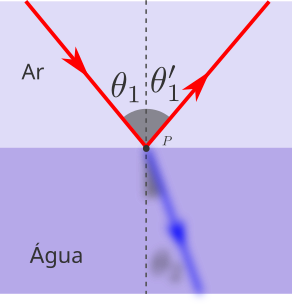
\includegraphics[width=1\textwidth]{img/reflexao.png}
    \caption{Lei da Reflexão}
    \label{fig:lei-da-reflexao}
    \tcblower
    \emph{Matematicamente:}
    \begin{align}
        \theta_1=\theta_1^{\prime }               
    \end{align}
  \end{mybox}    
\end{wrapfigure}
Vimos através da simulação do \emph{PheT}, que quando um feixe de luz incide sobre uma interface que separa dois meios físicos transparentes diferentes, a trajetória deste feixe sofre reflexão assim que encontra a interface, e um desvio ao entrar no meio. O ângulo que o raio incidente faz com a normal à superfície é sempre igual ao ângulo que o raio refletido também faz com a normal, está observação é conhecida normalmente como \emph{Lei da Reflexão}. A \autoref{fig:lei-da-reflexao} ao lado ilustra o caso.       

Já para o raio incidente e o refratado, podemos afirmar que, dependendo de em qual meio o feixe de luz está vindo e pra qual meio ele está indo, o feixe sofrerá um desvio que irá se aproximar da reta normal à superfície, ou se afastar dela, isto se deve ao fato de que a luz, ao passar de um meio para o outro, não altera a sua frequência, veremos mais adiante que como consequência disso, o comprimento de onda e a velocidade da onda sofrem mudanças na passagem entre os meios, provocando o desvio original de sua trajetória. A \autoref{fig:refracao} mostra o que observamos na simulação.

\vspace{5pt}
\begin{figure}[!ht]        
    \centering              
    \subfloat[Trajetória da luz partindo do ar para água \label{fig:refracao-a}]{
        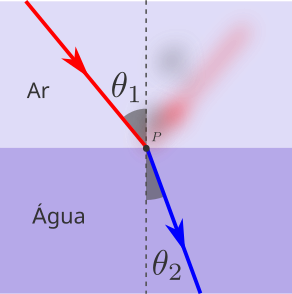
\includegraphics[width=.45\textwidth]{img/refracao-1a.png}
    }\hfill
    \subfloat[Trajetória da luz partindo da água para o ar \label{fig:refracao-b}]{
        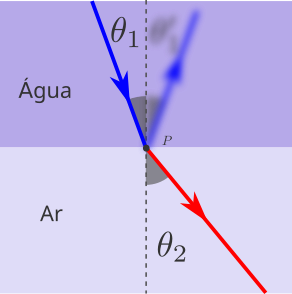
\includegraphics[width=.45\textwidth]{img/refracao-1b.png}
    }        
    \caption{Diagrama ilustrando um feixe de luz incidente e refratado na travessia entre dois meios ópticos ar e água, a seta indica a direção de propagação do feixe. Em (a) o feixe refratado está mais próximo da reta normal que o feixe incidente, o ângulo $\theta_1$ é maior que o ângulo $\theta_2$, já em (b) a situação se inverte quando invertemos os meios.}
    \label{fig:refracao}
  \end{figure}
\vspace*{20pt}

Embora seja possível explicar o fenômeno da refração pelo modelo corpuscular \emph{(possível porém nada simples)}, os resultados previstos diferem do que hoje é conhecido. A teoria corpuscular, prevê que a velocidade da luz deve ser \emph{maior} na água do que no ar, o que não é verdade! Por isso, o modelo ondulatório é mais correto para a descrição deste fenômeno, a seguir, usaremos o que aprendemos sobre ondas, para encontrar uma relação entre o ângulo incidente $\theta_1$ e o ângulo refratado $\theta_2$.


\subsection*{Índice de refração}        

Já vimos que os ângulos de incidência e refração, serão diferentes dependendo de cada meio físico e que tem relação direta com a velocidade da luz em cada meio. Convenientemente define-se uma grandeza auxiliar chamada de \textbf{índice de refração} $n$, cada meio possui um índice de refração associado e tem a ver com as propriedades físicas do material.

A relação entre o índice de refração e a velocidade da luz em um meio qualquer, é a razão entre a velocidade da luz em um meio conhecido e a velocidade da luz no meio em que a luz refrata. Um meio em que já se conhece bem como é a velocidade da luz é o vácuo e vale $c$ como já vimos anteriormente, por definição escreve-se o \textbf{índice de refração absoluto} como sendo:

\begin{align}
    n&=\frac{c}{v}
\end{align}
com
\begin{itemize}
    \item $n$: índice de refração absoluto;
    \item $c$: a velocidade da luz no vácuo ($c\simeq 3,0\times 10^8\mps$)
    \item $v$: a velocidade da luz no meio refratado.
\end{itemize}
\begin{mybox}[colback=white, colframe=darkpastelblue,colbacktitle=darkpastelblue!85!darkpastelblue,]{Exemplo Resolvido}
    \textbf{Calculando o índice de refração do ar:} Já foi determinado experimentalmente a velocidade da luz no ar, seu valor é $v_{\mathrm{ar}}=299\;705\;543,4\mps$. Calcular o índice de refração absoluto para o meio (ar), é só fazer a razão entre a velocidade da luz no vácuo $c=299\;792\;458\mps$ e $v_{\mathrm{ar}}$, segue que:

    \tcblower
    \begin{align}
        \begin{split}
            n_{\mathrm{ar}}&=\frac{c}{v_{\mathrm{ar}}}\\
            n_{\mathrm{ar}}&=\frac{299\;792\;458\mps}{299\;705\;543,4\mps}\\
            n_{\mathrm{ar}}&=1,00029\
        \end{split}
    \end{align}
    Por causa dessa proximidade entre a velocidade da luz no vácuo e no ar, convenciona-se que o índice de refração da luz no ar é $n_{\mathrm{ar}}=1,0$ igual ao do vácuo.        
\end{mybox}

\subsection*{Lei de Snell-Descartes}

Willebrord Snel van Royen (1580--1626) foi um matemático e astrônomo Holandês a quem atribui-se a descoberta da famosa \emph{Lei de Snell-Descartes} (também conhecida por \emph{Lei de Snell}).

Até a publicação do livro Optics de Huygens, a lei era atribuída somente a Descartes, porém, como a resolução de Descartes usou diversas suposições erradas, além de não haver nenhuma comprovação experimental, foram feitas acusações de que ele haveria forçado sua resolução a aproximar-se da de Snell. Contudo, nem Snell nem Descartes foram os primeiros a descobri-la e sim, um físico e matemático persa, que viveu entre os anos 940 e 1000 chamado Ibn Sahl, cujo o qual obteve resultados mais próximos dos que se conhece hoje em dia, porém sua pesquisa sobre a lei da refração não foi explicitada em seus trabalhos, ficando esquecida até meados do século XX.        

É possível deduzir a lei de Snell a partir dos conceitos estudados até aqui, para isso, vamos novamente relembrar da simulação feita na primeira aula.

Um feixe de luz propagando-se em um meio, que vamos chamar de meio \ding{192}, incide sobre uma superfície que separa este meio de um segundo, o meio \ding{193}. Sendo eles diferentes entre si, vimos que o feixe de luz tende a se comportar de duas formas: afastado-se da reta normal ao ponto em que houve o contato do feixe com a superfície, ou aproximando-se dela.

Vamos inicialmente supor que ao passar para o meio \ding{193}, o feixe aproxima-se da reta normal formando um ângulo de refração $\theta_2$. Se $\theta_1$ é o ângulo de incidência então $\theta_1>\theta_2$ por hipótese. A Figura\autoref{fig:snell-1} ilustra o caso.

\vspace{5pt}
\begin{figure}[!ht]        
    \centering              
    \subfloat[\label{fig:snell-1}]{
        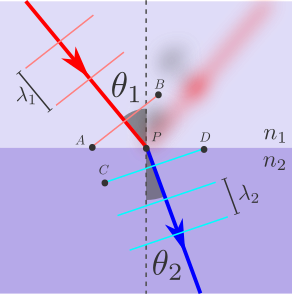
\includegraphics[width=.4\textwidth]{img/snell-1.png}
    }\hspace{20pt}
    \subfloat[\label{fig:snell-2}]{
        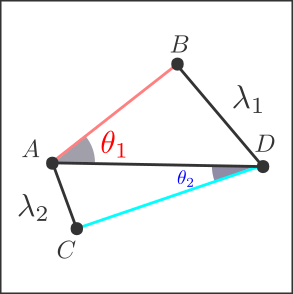
\includegraphics[width=.4\textwidth]{img/snell-2.png}
    }        
    \caption{Esquema representativo da refração da luz em dois meios diferentes. Em (a) o feixe propaga-se do meio \ding{192} para o meio \ding{193}, as frentes de onda estão representadas por retas perpendiculares à direção de propagação do feixe, como por exemplo a reta $\overline{AB}$ e $\overline{CD}$. Já em (b), tem-se um diagrama formado ligando os pontos $A$, $B$, $D$, $C$ e $A$ da Figura\autoref{fig:snell-1}, obtem-se assim, dois triângulos retângulos conectados pela hipotenusa $\overline{AD}$.}
    \label{fig:snell}
  \end{figure}        
  \vspace*{20pt}
  
  Na figura acima, o segmento de reta $\overline{AB}$ representa um pulso da onda luminosa no meio \ding{192}, a distância entre um pulso e outro nesse meio equivale a um comprimento de onda $\lambda_1$, o pulso seguinte encontra-se no meio \ding{193} e está representado pelo segmento de reta $\overline{CD}$, nesse meio a distância entre cada pulso é de $\lambda_2$. Cada parte do pulso $\overline{AB}$ ao entrar no meio \ding{193} é reorientado de forma que permaneça perpendicular à direção de propagação do feixe, assim, quando o ponto $A$ chegar no ponto $C$ o ponto $B$ também deve localizar-se no ponto $D$.

  Conectando os pontos $A$, $B$, $C$ e $D$, obtemos a Figura\autoref{fig:snell-2}. Do triângulo retângulo $\triangle ABD$ temos:
  \begin{align}
    \sin\theta_1&=\frac{\lambda_1}{\overline{AD}}
  \end{align}
  e do triângulo retângulo $\triangle ACD$ temos:
  \begin{align}
    \sin\theta_2&=\frac{\lambda_2}{\overline{AD}}
  \end{align}
  dividindo $\sin\theta_1$ por $\sin\theta_2$ chegamos a seguinte relação
  \begin{align}
    \begin{split}
        \frac{\sin\theta_1}{\sin\theta_2}&=\frac{\lambda_1}{\overline{AD}}\frac{\overline{AD}}{\lambda_2}\\
        \frac{\sin\theta_1}{\sin\theta_2}&=\frac{\lambda_1}{\lambda_2}
    \end{split}
  \end{align}
Algumas conclusões pode-se tirar da relação acima, por exemplo:
\begin{itemize}
    \item Se $\theta_1>\theta_2$ então $\lambda_1>\lambda_2$, ou seja, se o raio refratado sofre desvio aproximando-se da normal ($\theta_1>\theta_2$), o comprimento de onda da luz refratada é diminuído proporcionalmente ($\lambda_1>\lambda_2$).
    \item Analogamente, se $\theta_1<\theta_2$ então $\lambda_1<\lambda_2$, se o raio refratado sofre desvio afastando-se da normal ($\theta_1<\theta_2$), seu comprimento de onda sofre um alargamento ($\lambda_1<\lambda_2$). 
\end{itemize}


Isso explica alguns fenômenos que observamos cotidianamente por exemplo: porque o céu é azul durante o dia e vermelho ao entardecer, porque observamos as cores do arco-íris e a dispersão da luz em prismas, sempre numa certa ordem, veja a \autoref{fig:dispersao} a seguir:
\vspace{5pt}
\begin{figure}[!ht]        
    \centering              
    \subfloat[\label{fig:arco-iris}]{
        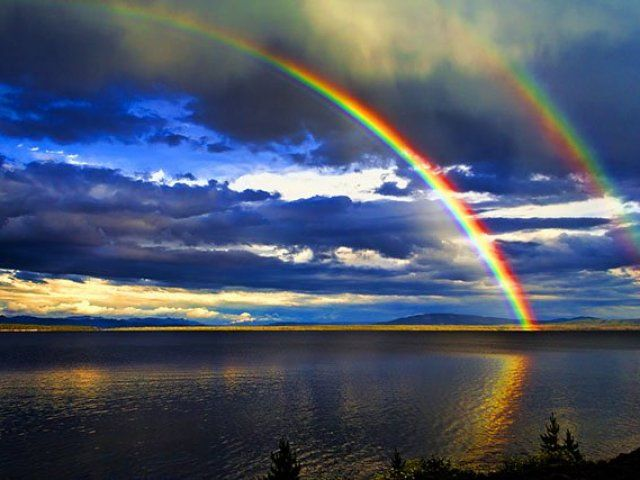
\includegraphics[width=.4\textwidth]{img/arco-iris.jpg}
    }\hspace{20pt}
    \subfloat[\label{fig:prisma-de-newton}]{
        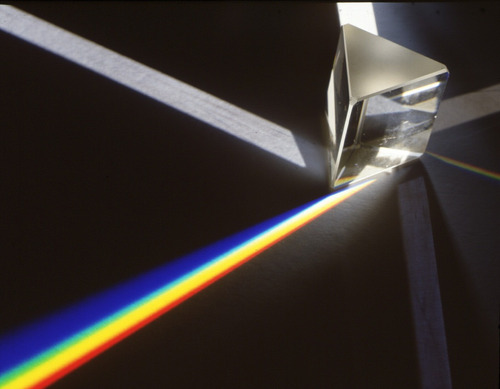
\includegraphics[width=.4\textwidth]{img/prisma.jpg}
    }        
    \caption{Fenêmeno de dispersão observado em (a) formação do arco-íris e (b) prisma de Newton. Se quiser saber sobre este assunto clique \href{https://www.bbc.com/portuguese/curiosidades-49906709}{aqui}}
    \label{fig:dispersao}
\end{figure}        
\vspace*{20pt}

Mas o que podemos dizer sobre a velocidade da luz? Sendo a luz um tipo de onda, vimos na seção \ref{sec:velocidade-da-onda} como calcular a sua velocidade em termos do comprimento de onda e da frequência da luz, $v=\lambda f$, se isso é verdade então podemos escrever a relação que encontramos como sendo a seguinte
\begin{align}
    \begin{split}
        \label{eq:lei-snell-frequencia}
        \frac{\sin\theta_1}{\sin\theta_2}&=\frac{\lambda_1}{\lambda_2}\\
        \frac{\sin\theta_1}{\sin\theta_2}&=\left(\frac{v_1}{f_1}\right)\left(\frac{f_2}{v_2}\right)
    \end{split}
\end{align}
Se tratando de luz monocromática, o feixe incidente é o mesmo feixe refratado no material, apenas com o comprimento de onda diferente, nesse caso a sua frequência de oscilação $f$ continua a mesma, ou seja $f_1=f_2=f$, \textbf{a frequência de uma onda monocromática nunca muda!} Então, reescrevemos a relação \eqref{eq:lei-snell-frequencia} como sendo:
\begin{align}
    \begin{split}
        \frac{\sin\theta_1}{\sin\theta_2}&=\left(\frac{v_1}{f}\right)\left(\frac{f}{v_2}\right)\\
        \frac{\sin\theta_1}{\sin\theta_2}&=\frac{v_1}{v_2}\label{eq:lei-snell-velocidades}
    \end{split}
\end{align}
E novamente,
\begin{itemize}
    \item Se o raio refratado se aproxima da normal $\theta_1>\theta_2$ a velocidade da onda refratada é \textbf{menor} que a velocidade da onda incidente $v_1>v_2$. Isto contraria a previsão feita pelo modelo corpuscular e por isso este modelo não é apropriado para descrever o fenômeno de refração!
    \item De outro modo, se o raio refratado se afasta da normal $\theta_1<\theta_2$, indicando que a velocidade do feixe de luz refratado é \textbf{maior} do que a velocidade do feixe incidente.
\end{itemize}
estes são os resultados previstos pela Lei de Snell-Descartes. Há uma forma de representar estes resultados em termos dos índices de refração de cada material, vamos retomar a equação \eqref{eq:lei-snell-velocidades} e reescrevê-la de uma forma em que tudo o que diz respeito a onda incidente fique de um lado da igualdade e tudo o que diz respeito a parte refratada da onda fique do outro lado
\begin{align}
    \begin{split}
        \frac{\sin\theta_1}{\sin\theta_2}&=\frac{v_1}{v_2}\\
        \frac{1}{v_1}\sin\theta_1&=\frac{1}{v_2}\sin\theta_2
    \end{split}
\end{align}
Agora é só multiplicarmos os dois lados da igualdade acima pela constate $c$ que representa a velocidade da luz, lembrando que a razão $c/v$ é definida como o índice de refração $n$, então
\begin{align}
    \begin{split}
        \frac{1}{v_1}\sin\theta_1&=\frac{1}{v_2}\sin\theta_2\\
        \frac{c}{v_1}\sin\theta_1&=\frac{c}{v_2}\sin\theta_2\\                                             
    \end{split}                                   
\end{align}
Assim, a forma mais conhecida da Lei de Snell-Descartes é dada por
\begin{align}
    \boxed{
        n_1\sin\theta_1=n_2\sin\theta_2
    } 
\end{align} 
    \newpage
    \begin{center}
    \section{Lista de Exercícios}    
\end{center}

\subsection{Questões}

\begin{quest}
    A Física utiliza de modelos abstratos para explicar os fenômenos da natureza, o modelo Partícula (ou corpuscular) e o modelo Ondulatório são dois exemplos destes modelos. Cite as principais diferenças entre o modelo Partícula e o Modelo Ondulatório.
\end{quest}
\begin{quest}
    Por que o fenômeno da refração não pode ser explicado pelo Modelo Partícula?            
\end{quest}
% \begin{quest}
%     Por que o céu é azul durante o dia e alaranjado/avermelhado ao final da tarde? (Pesquise.)
% \end{quest}
\begin{quest}
    Se o índice de refração $n_1$ cujo o qual tem-se origem um feixe de luz é obrigatoriamente o ar, qual deve ser a direção de propagação do feixe refratado em um meio qualquer de índice de refração $n_2$?
\end{quest}
\begin{quest}
    A partir da \autoref{fig:questao-5} a seguir, responda as questões
    \vspace*{30pt}
    \begin{figure}[ht!]
        \centering
        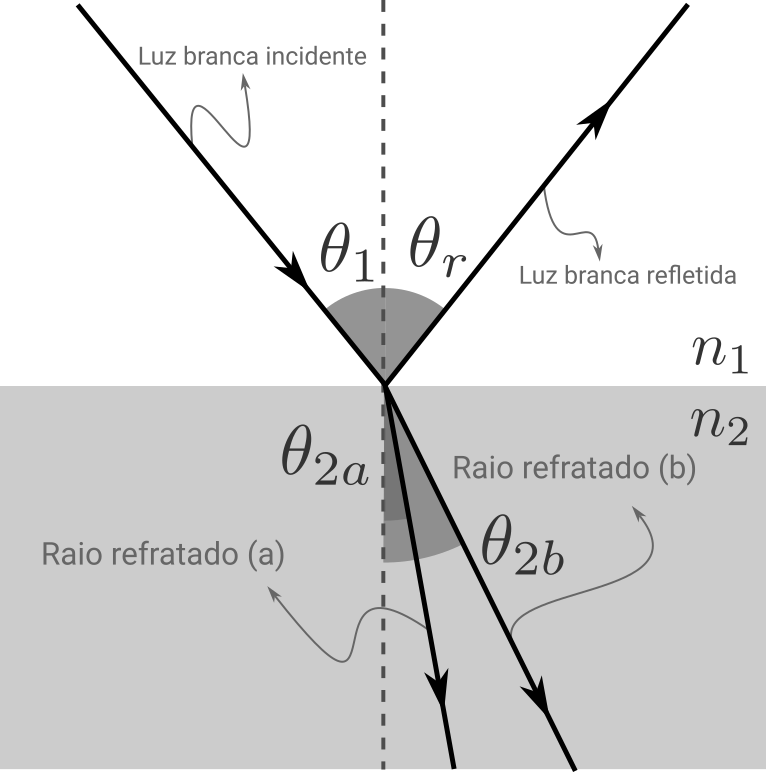
\includegraphics[width=.6\textwidth]{img/questao-5.png}
        \caption{Dispersão da luz branca em um meio material de índice de refração $n_2$}
        \label{fig:questao-5}  
    \end{figure}
    \vspace*{20pt}
    \begin{enumerate}[label=\alph *)]
        \item Se $\theta_r$ é o ângulo da luz refletida, o que pode-se afirmar sobre $\theta_r$ com relação ao ângulo de incidência $\theta_1$?
        \item Dentre os índices de refração $n_1$ e $n_2$ qual é o maior? (Justifique!)
        \item Supondo que ocorra o fenômeno de dispersão máxima entre os raios refratados, qual deve ser a cor do raio refratado ($a$) e do raio refratado ($b$), respectivamente? (Justifique!)
    \end{enumerate}        
\end{quest}

\subsection{Problemas}

\begin{prob}
    Um feixe de luz monocromático incide sobre uma superfície de separação entre dois meios. O meio 1 (incidente) possui índice de refração $n_1$, o meio 2 (refratado) possui índice de refração $n_2$. Se os ângulos de incidência e de refração são respectivamente $\theta_1=30^{\circ}$ e $\theta_2=45^{\circ}$, determine a razão entre $n_1$ e $n_2$.
\end{prob}
\begin{prob}
    Uma raio de luz monocromático propaga-se de um meio cujo o índice de refração vale $n_1$, para um outro meio de índice de refração $n_2=1,00$, formando com a normal à superfície ângulos de $\theta_1=30^{\circ}$ (incidente) e $\theta_2=45^{\circ}$ (refratado). Qual a velocidade da luz no meio incidente $n_1$?
\end{prob}
\begin{prob}(ENEM)
     A \autoref{fig:problema-3} representa um prisma óptico, constituído de um material transparente, cujo índice de refração é crescente com a frequência da luz que sobre ele incide. Um feixe luminoso, composto por luzes vermelha, azul e verde, incide na face $A$, emerge na face $B$ e, após ser refletido por um espelho, incide num filme para fotografia colorida, revelando três pontos.

    \vspace{20pt}
    \begin{figure}[ht!]
        \centering
        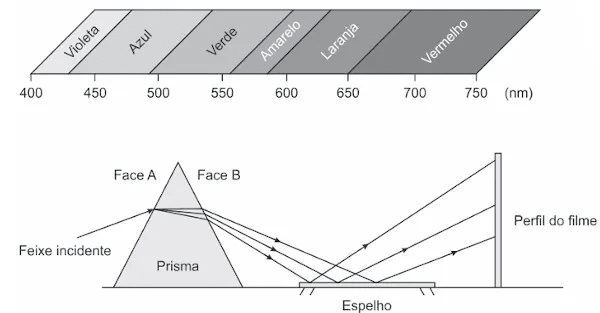
\includegraphics[width=.6\textwidth]{img/problema-3.png}
        \caption{Dispersão da luz em um prisma.}
        \label{fig:problema-3}                
    \end{figure}
    \vspace{20pt}
    \noindent Observando os pontos luminosos revelados no filme, de baixo para cima, constatam-se as seguintes cores:
    \begin{enumerate}[label=\alph *)]
        \item vermelha, verde, azul.
        \item verde, vermelha, azul.
        \item azul, verde, vermelha.
        \item verde, azul, vermelha.
        \item azul, vermelha, verde.
    \end{enumerate}
\end{prob}
\begin{prob}(ENEM)
    Alguns povos indígenas ainda preservam suas tradições realizando a pesca com lanças, demonstrando uma notável habilidade. Para fisgar um peixe em um lago com águas tranquilas o índio deve mirar abaixo da posição em que enxerga o peixe.

    \noindent Ele deve proceder dessa forma porque os raios de luz:
    \begin{enumerate}[label=\alph *)]
        \item refletidos pelo peixe não descrevem uma trajetória retilínea no interior da água.
        \item emitidos pelos olhos do índio desviam sua trajetória quando passam do ar para a água.
        \item espalhados pelo peixe são refletidos pela superfície da água.
        \item emitidos pelos olhos do índio são espalhados pela superfície da água.
        \item refletidos pelo peixe desviam sua trajetória quando passam da água para o ar.
    \end{enumerate}
\end{prob}
\begin{prob}(UDESC)
    Considere uma lâmina de vidro de faces paralelas imersa no ar. Um raio luminoso propaga-se no ar e incide em uma das faces da lâmina, segundo um ângulo  $\theta$ em relação à direção normal ao plano da lâmina. O raio é refratado nesta face e refletido na outra face, que é espelhada. O raio refletido é novamente refratado na face não espelhada, voltando a propagar-se no ar. Sendo $n_{a}$ e $n_{v}$   respectivamente, os índices de refração da luz no ar e no vidro, o ângulo de refração $\alpha$ que o raio refletido forma no vidro, com a direção normal ao plano da lâmina, ao refratar-se pela segunda vez, obedece à equação:
    \begin{enumerate}[label=\alph *)]
        \item $n_{v}\sin\alpha=n_{a}\sin(\theta /2)$
        \item $\alpha=\theta$
        \item $\sin\alpha=\cos\theta$
        \item $n_v\sin\alpha=n_a\sin\theta$
        \item $n_a\sin\alpha=n_v\sin\theta$
    \end{enumerate}
\end{prob}
\end{apendicesenv}
%-----------------------------------------------%
% Anexos
%-----------------------------------------------%
%-----------------------------------------------%
% Plano de Aula 01
%-----------------------------------------------%
\begin{anexosenv}     
    % \chapter{Acompanhamento de Aulas}
    % \begin{landscape}    
    % \end{landscape}
    % \chapter{Cronograma de aulas}
    % 	\includepdf[pages=-]{03-pos-textual/cronograma.pdf}
    \chapter{Materiais da Turma}
    \thispagestyle{empty}
    \label{anx:materiaisAnexo}
    
    \section{Unidade: Dilatação Térmica}
    \label{anx:materialAnexoDilatacaoTermica}
    Material de apoio desenvolvido pelo professor supervisor, para suporte às aulas de Dilatação Térmica. Este material encontra-se disponível para a turma no ambiente de ensino virtual \emph{Google Classroom} destacado pelo retângulo em vermelho na \autoref{fig:gClassroom}
    \vspace{1cm}
    \begin{figure}[!h]
        \centering
        \footnotesize        
        \caption{Print Screen do Google Classroom da Turma 2(5)}
        \includegraphics[width=\textwidth]{03-elementos/03.2_textual/03.2.1_fig/google-class01.png}
        \label{fig:gClassroom}
    \end{figure}

    Segue na integra:
    \includepdf[pages=-,scale=1]{03-elementos/03.2_textual/03.2.1_fig/apendice-I}
    % \includecode[shell]{l_olamundo}{Olá mundo em shell script}{03-elementos/03.2_textual/03.2.0_codes/ola.sh}

    % ROTEIROS EXPERIMENTAIS
    \chapter{Roteiros Experimentais}
    \label{anx:roteiros-experimentais}
    \section{Invisibilidade Observada Devido à Refração}
    \label{anx:invisibilidade-refracao}
    \subsection*{Materiais:}
    \begin{itemize}
        \item 1 béquer com $250\,\mathrm{ml}$ de água;
        \item 1 béquer com $250\,\mathrm{ml}$ de glicerina;
        \item 2 béquer de capacidade $50\,\mathrm{ml}$ vazio;
        \item 1 béquer com $500\,\mathrm{ml}$ de óleo de soja;
        \item 2 tubos de ensaio;
        \item 2 bastões de vidro;
        \item 1 pinça.
    \end{itemize}
    \subsection*{Procedimento:}
    \begin{enumerate}
        \item Introduzir o bastão de vidro primeiro na água e depois na glicerina e observar;
        \item Preencher um tubo de ensaio com óleo e inserir no béquer de $500\,\mathrm{ml}$ de óleo;
        \item No mesmo béquer de $500\,\mathrm{ml}$ de óleo, inserir outro tubo de ensaio vazio e comparar com o tubo de ensaio que está cheio de óleo;
        \item No tubo de ensaio vazio, que está dentro do béquer com óleo, colocar água lentamente até a metade do tubo e observar;
        \item Ainda no tubo de ensaio contendo água, preencher lentamente com óleo e observar. 
    \end{enumerate}
    \subsection*{Questões:}
    \begin{quest}
        Por que o bastão de vidro "desaparece" quando colocamos na glicerina?
    \end{quest}
    \begin{quest}
        Como explicar o fato do tubo de ensaio desaparecer quando inserimos óleo?
    \end{quest}
\end{anexosenv}
%-----------------------------------------------%
% INDICE REMISSIVO
%-----------------------------------------------%
\phantompart
\printindex
%-----------------------------------------------%
\end{document}


